\documentclass[]{article}
\usepackage{lmodern}
\usepackage{amssymb,amsmath}
\usepackage{ifxetex,ifluatex}
\usepackage{fixltx2e} % provides \textsubscript
\ifnum 0\ifxetex 1\fi\ifluatex 1\fi=0 % if pdftex
  \usepackage[T1]{fontenc}
  \usepackage[utf8]{inputenc}
\else % if luatex or xelatex
  \ifxetex
    \usepackage{mathspec}
  \else
    \usepackage{fontspec}
  \fi
  \defaultfontfeatures{Ligatures=TeX,Scale=MatchLowercase}
\fi
% use upquote if available, for straight quotes in verbatim environments
\IfFileExists{upquote.sty}{\usepackage{upquote}}{}
% use microtype if available
\IfFileExists{microtype.sty}{%
\usepackage{microtype}
\UseMicrotypeSet[protrusion]{basicmath} % disable protrusion for tt fonts
}{}
\usepackage[margin=1in]{geometry}
\usepackage{hyperref}
\hypersetup{unicode=true,
            pdftitle={All Countries Environmental Data},
            pdfborder={0 0 0},
            breaklinks=true}
\urlstyle{same}  % don't use monospace font for urls
\usepackage{color}
\usepackage{fancyvrb}
\newcommand{\VerbBar}{|}
\newcommand{\VERB}{\Verb[commandchars=\\\{\}]}
\DefineVerbatimEnvironment{Highlighting}{Verbatim}{commandchars=\\\{\}}
% Add ',fontsize=\small' for more characters per line
\usepackage{framed}
\definecolor{shadecolor}{RGB}{248,248,248}
\newenvironment{Shaded}{\begin{snugshade}}{\end{snugshade}}
\newcommand{\AlertTok}[1]{\textcolor[rgb]{0.94,0.16,0.16}{#1}}
\newcommand{\AnnotationTok}[1]{\textcolor[rgb]{0.56,0.35,0.01}{\textbf{\textit{#1}}}}
\newcommand{\AttributeTok}[1]{\textcolor[rgb]{0.77,0.63,0.00}{#1}}
\newcommand{\BaseNTok}[1]{\textcolor[rgb]{0.00,0.00,0.81}{#1}}
\newcommand{\BuiltInTok}[1]{#1}
\newcommand{\CharTok}[1]{\textcolor[rgb]{0.31,0.60,0.02}{#1}}
\newcommand{\CommentTok}[1]{\textcolor[rgb]{0.56,0.35,0.01}{\textit{#1}}}
\newcommand{\CommentVarTok}[1]{\textcolor[rgb]{0.56,0.35,0.01}{\textbf{\textit{#1}}}}
\newcommand{\ConstantTok}[1]{\textcolor[rgb]{0.00,0.00,0.00}{#1}}
\newcommand{\ControlFlowTok}[1]{\textcolor[rgb]{0.13,0.29,0.53}{\textbf{#1}}}
\newcommand{\DataTypeTok}[1]{\textcolor[rgb]{0.13,0.29,0.53}{#1}}
\newcommand{\DecValTok}[1]{\textcolor[rgb]{0.00,0.00,0.81}{#1}}
\newcommand{\DocumentationTok}[1]{\textcolor[rgb]{0.56,0.35,0.01}{\textbf{\textit{#1}}}}
\newcommand{\ErrorTok}[1]{\textcolor[rgb]{0.64,0.00,0.00}{\textbf{#1}}}
\newcommand{\ExtensionTok}[1]{#1}
\newcommand{\FloatTok}[1]{\textcolor[rgb]{0.00,0.00,0.81}{#1}}
\newcommand{\FunctionTok}[1]{\textcolor[rgb]{0.00,0.00,0.00}{#1}}
\newcommand{\ImportTok}[1]{#1}
\newcommand{\InformationTok}[1]{\textcolor[rgb]{0.56,0.35,0.01}{\textbf{\textit{#1}}}}
\newcommand{\KeywordTok}[1]{\textcolor[rgb]{0.13,0.29,0.53}{\textbf{#1}}}
\newcommand{\NormalTok}[1]{#1}
\newcommand{\OperatorTok}[1]{\textcolor[rgb]{0.81,0.36,0.00}{\textbf{#1}}}
\newcommand{\OtherTok}[1]{\textcolor[rgb]{0.56,0.35,0.01}{#1}}
\newcommand{\PreprocessorTok}[1]{\textcolor[rgb]{0.56,0.35,0.01}{\textit{#1}}}
\newcommand{\RegionMarkerTok}[1]{#1}
\newcommand{\SpecialCharTok}[1]{\textcolor[rgb]{0.00,0.00,0.00}{#1}}
\newcommand{\SpecialStringTok}[1]{\textcolor[rgb]{0.31,0.60,0.02}{#1}}
\newcommand{\StringTok}[1]{\textcolor[rgb]{0.31,0.60,0.02}{#1}}
\newcommand{\VariableTok}[1]{\textcolor[rgb]{0.00,0.00,0.00}{#1}}
\newcommand{\VerbatimStringTok}[1]{\textcolor[rgb]{0.31,0.60,0.02}{#1}}
\newcommand{\WarningTok}[1]{\textcolor[rgb]{0.56,0.35,0.01}{\textbf{\textit{#1}}}}
\usepackage{graphicx,grffile}
\makeatletter
\def\maxwidth{\ifdim\Gin@nat@width>\linewidth\linewidth\else\Gin@nat@width\fi}
\def\maxheight{\ifdim\Gin@nat@height>\textheight\textheight\else\Gin@nat@height\fi}
\makeatother
% Scale images if necessary, so that they will not overflow the page
% margins by default, and it is still possible to overwrite the defaults
% using explicit options in \includegraphics[width, height, ...]{}
\setkeys{Gin}{width=\maxwidth,height=\maxheight,keepaspectratio}
\IfFileExists{parskip.sty}{%
\usepackage{parskip}
}{% else
\setlength{\parindent}{0pt}
\setlength{\parskip}{6pt plus 2pt minus 1pt}
}
\setlength{\emergencystretch}{3em}  % prevent overfull lines
\providecommand{\tightlist}{%
  \setlength{\itemsep}{0pt}\setlength{\parskip}{0pt}}
\setcounter{secnumdepth}{0}
% Redefines (sub)paragraphs to behave more like sections
\ifx\paragraph\undefined\else
\let\oldparagraph\paragraph
\renewcommand{\paragraph}[1]{\oldparagraph{#1}\mbox{}}
\fi
\ifx\subparagraph\undefined\else
\let\oldsubparagraph\subparagraph
\renewcommand{\subparagraph}[1]{\oldsubparagraph{#1}\mbox{}}
\fi

%%% Use protect on footnotes to avoid problems with footnotes in titles
\let\rmarkdownfootnote\footnote%
\def\footnote{\protect\rmarkdownfootnote}

%%% Change title format to be more compact
\usepackage{titling}

% Create subtitle command for use in maketitle
\newcommand{\subtitle}[1]{
  \posttitle{
    \begin{center}\large#1\end{center}
    }
}

\setlength{\droptitle}{-2em}

  \title{All Countries Environmental Data}
    \pretitle{\vspace{\droptitle}\centering\huge}
  \posttitle{\par}
    \author{}
    \preauthor{}\postauthor{}
    \date{}
    \predate{}\postdate{}
  

\begin{document}
\maketitle

\hypertarget{method-pca}{%
\subsection{Method: PCA}\label{method-pca}}

Principal component analysis (PCA), part of descriptive analytics, is
used to analyze one table of quantitative data, specifically useful for
\emph{high dimensional data} and comparitively lesser data rows. PCA
mixes the input variables to give new variables, called principal
components. The first principal component is the line of best fit. It is
the line that maximizes the inertia (similar to variance) of the cloud
of data points. Subsequent components are defined as orthogonal to
previous components, and maximize the remaining inertia.

PCA gives one map for the rows (called factor scores), and one map for
the columns (called loadings). These 2 maps are related, because they
both are described by the same components. However, these 2 maps project
different kinds of information onto the components, and so they are
\emph{interpreted differently}. Factor scores are the coordinates of the
row observations and Loadings describe the column variables. Both can be
interpreted through their distance from origin. However, Factor scores
are also interpreted by the distances between them and Loadings
interpreted by the angle between them.

The distance from the origin is important in both maps, because squared
distance from the mean is inertia (variance, information; see sum of
squares as in ANOVA/regression). Because of the Pythagorean Theorem, the
total information contributed by a data point (its squared distance to
the origin) is also equal to the sum of its squared factor scores.

With both Factor and Loadings maps combined we can interpret which
grouping criteria of rows of data is most impacted by which columns.
This can interpreted visually by observing which a factors and loadings
on a particular component and the distance on this component.

PCA also helps in \emph{dimensionality reduction}. Using SVD, we get
eigen values arranged in descending order in the diagonal matrix. We can
simply ignore the lower eigen values to reduce dimensions. We can also
take help of SCREE plot to visually analyze importance of eigen values.

\hypertarget{dataset}{%
\subsection{Dataset}\label{dataset}}

\begin{itemize}
\item
  Data: Measurements of environment conditions in Countries
\item
  Rows: There are 137 observations, 1 for each country.
\item
  Columns: Total 29 variables
\item
  Qualitative: Country (nominal), Happiness (Ordinal).
\item
  Quantitative: Aspect, Slope Crop Land, Tree Canopy Wind Cloud \&
  Multiple variables for Temp \& Rain
\item
  Structure of Data
\end{itemize}

\begin{Shaded}
\begin{Highlighting}[]
\KeywordTok{str}\NormalTok{(country_env_df)}
\end{Highlighting}
\end{Shaded}

\begin{verbatim}
## 'data.frame':    137 obs. of  29 variables:
##  $ Country                : Factor w/ 137 levels "Afghanistan",..: 1 2 3 4 5 6 7 8 9 10 ...
##  $ Happiness_Rank         : Ord.factor w/ 3 levels "VH"<"H"<"U": 3 2 2 3 1 3 1 1 2 2 ...
##  $ accessibility_to_cities: num  317.7 73.8 1212.8 378.2 209.2 ...
##  $ elevation              : num  1832 652 557 1061 683 ...
##  $ aspect                 : num  201 192 185 174 145 ...
##  $ slope                  : num  1.516 1.89 0.171 0.193 0.624 ...
##  $ cropland_cover         : num  9.51 23.35 3.69 2.79 21.96 ...
##  $ tree_canopy_cover      : num  0.375 12.805 0.177 19.87 8.834 ...
##  $ isothermality          : num  35.9 33.2 40.3 64.3 49.9 ...
##  $ rain_coldestQuart      : num  128.72 392.51 25.29 8.05 79.09 ...
##  $ rain_driestMonth       : num  1.722 40.088 0.935 0.26 17.183 ...
##  $ rain_driestQuart       : num  8.3 138.15 6.09 4.43 60.49 ...
##  $ rain_mean_annual       : num  311.3 1151.1 79.5 1023.4 539.9 ...
##  $ rain_seasonailty       : num  91.6 38.5 67.1 91.5 48.3 ...
##  $ rain_warmestQuart      : num  12.69 138.33 9.51 318.54 183.14 ...
##  $ rain_wettestMonth      : num  67.8 159 13.4 202.2 79.2 ...
##  $ rain_wettestQuart      : num  175.8 435.9 33.3 524.3 211.7 ...
##  $ temp_annual_range      : num  40.3 27.1 36.5 21.5 26.8 ...
##  $ temp_coldestQuart      : num  -0.261 3.58 13.152 18.794 8.024 ...
##  $ temp_diurnal_range     : num  14.72 9.11 14.87 13.85 13.46 ...
##  $ temp_driestQuart       : num  21.1 19.6 26.9 18.9 11.1 ...
##  $ temp_max_warmestMonth  : num  32 26.3 41.5 31 28.2 ...
##  $ temp_mean_annual       : num  11.5 11.5 23 21.6 14.2 ...
##  $ temp_min_coldestMonth  : num  -8.312 -0.806 5.058 9.549 1.443 ...
##  $ temp_seasonality       : num  88.2 62.7 75.1 18.5 47.6 ...
##  $ temp_warmestQuart      : num  22.7 19.6 32.5 23.3 20.2 ...
##  $ temp_wettestQuart      : num  3.95 5.27 20.81 22.76 16.48 ...
##  $ wind                   : num  3.43 2.47 4.03 2.16 4.27 ...
##  $ cloudiness             : num  114.2 181.1 90.7 187.5 159 ...
\end{verbatim}

\begin{itemize}
\tightlist
\item
  Research Question
\end{itemize}

How do the 137 countries differ on these variables?

\hypertarget{analysis}{%
\subsection{Analysis}\label{analysis}}

There are multiple variables representing rain and Temp. Hence, for
analysis purposes, lets choose annual mean for Rain and Temp.

\hypertarget{correlation-plot}{%
\subsubsection{Correlation Plot}\label{correlation-plot}}

Visually analyze multicollinearity in the system. Analyze the

\begin{Shaded}
\begin{Highlighting}[]
\NormalTok{corr_result =}\StringTok{ }\KeywordTok{cor}\NormalTok{(country_env_df_for_corr)}
\KeywordTok{corrplot}\NormalTok{(corr_result,}\DataTypeTok{order =} \StringTok{'hclust'}\NormalTok{, }\DataTypeTok{addrect =} \DecValTok{7}\NormalTok{)}
\end{Highlighting}
\end{Shaded}

\includegraphics{Group1_Ritesh_Malaiya_PCA_Inference_World_env_vars_files/figure-latex/unnamed-chunk-4-1.pdf}

\hypertarget{identify-latent-components}{%
\subsubsection{Identify Latent
Components}\label{identify-latent-components}}

\hypertarget{pca}{%
\paragraph{PCA}\label{pca}}

\begin{Shaded}
\begin{Highlighting}[]
\NormalTok{country_env_pca <-}\StringTok{ }\KeywordTok{epPCA}\NormalTok{(}\DataTypeTok{DATA =}\NormalTok{ country_env_df_for_pca, }\DataTypeTok{center =} \OtherTok{TRUE}\NormalTok{, }\DataTypeTok{scale =} \StringTok{'SS1'}\NormalTok{, }\DataTypeTok{DESIGN =}\NormalTok{ country_env_df}\OperatorTok{$}\NormalTok{Happiness_Rank, }\DataTypeTok{graphs =} \OtherTok{FALSE}\NormalTok{)}
\end{Highlighting}
\end{Shaded}

Now we have Factor scores and Loadings. * Factor Scores are the new Data
points w.r.t. new Components achieved with help of SVD. * Loadings
represent correlation between variables w.r.t the choosen Components.
Can be interpreted in 3 ways + As slices of inertia of the contribution
data table w.r.t. the choosen Components + As correlation between
columns (features) of Original Data and Factor scores of each Components
(latent features). + As coefficients of optimal linear combination
i.e.~Right Sigular Vectors (Q matrix of SVD) \#\#\#\# Scree Plot

\hypertarget{scree-plot}{%
\paragraph{Scree Plot}\label{scree-plot}}

Gives amount of information explained by corresponding component. Gives
an intuition to decide which components best represent data in order to
answer the research question.

P.S. The most contribution component may not always be most useful for a
given research question.

\begin{Shaded}
\begin{Highlighting}[]
\NormalTok{PTCA4CATA}\OperatorTok{::}\KeywordTok{PlotScree}\NormalTok{(}\DataTypeTok{ev =}\NormalTok{ country_env_pca}\OperatorTok{$}\NormalTok{ExPosition.Data}\OperatorTok{$}\NormalTok{eigs)}
\end{Highlighting}
\end{Shaded}

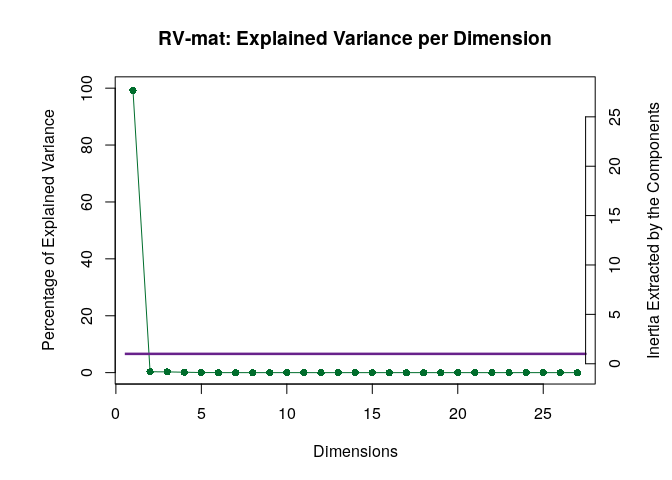
\includegraphics{Group1_Ritesh_Malaiya_PCA_Inference_World_env_vars_files/figure-latex/unnamed-chunk-5-1.pdf}

\hypertarget{factor-scores}{%
\paragraph{Factor Scores}\label{factor-scores}}

Lets visualize happiness categories for components 1-10, to make a
decision (visually) on the most important components.

\begin{Shaded}
\begin{Highlighting}[]
\ControlFlowTok{for}\NormalTok{(i }\ControlFlowTok{in} \KeywordTok{c}\NormalTok{(}\DecValTok{1}\NormalTok{,}\DecValTok{3}\NormalTok{,}\DecValTok{5}\NormalTok{,}\DecValTok{7}\NormalTok{, }\DecValTok{9}\NormalTok{)) \{}
\NormalTok{  axis1 =}\StringTok{ }\NormalTok{i}
\NormalTok{  axis2 =}\StringTok{ }\NormalTok{i}\OperatorTok{+}\DecValTok{1}

\NormalTok{  country_factor_map <-}\StringTok{ }\NormalTok{PTCA4CATA}\OperatorTok{::}\KeywordTok{createFactorMap}\NormalTok{(country_env_pca}\OperatorTok{$}\NormalTok{ExPosition.Data}\OperatorTok{$}\NormalTok{fi, }\DataTypeTok{title=}\StringTok{''}\NormalTok{, }
                                                 \DataTypeTok{col.points =}\NormalTok{ country_env_pca}\OperatorTok{$}\NormalTok{Plotting.Data}\OperatorTok{$}\NormalTok{fi.col,}
                                                 \DataTypeTok{col.labels =}\NormalTok{ country_env_pca}\OperatorTok{$}\NormalTok{Plotting.Data}\OperatorTok{$}\NormalTok{fi.col,}
                                                 \DataTypeTok{axis1 =}\NormalTok{ axis1,}
                                                 \DataTypeTok{axis2 =}\NormalTok{ axis2,}
                                                 \DataTypeTok{display.labels =} \OtherTok{FALSE}\NormalTok{)}

\NormalTok{country_factor_map_mean <-}\StringTok{ }\NormalTok{PTCA4CATA}\OperatorTok{::}\KeywordTok{createFactorMap}\NormalTok{(country_env_pca_mean,}
                                                 \DataTypeTok{col.points =} \KeywordTok{unique}\NormalTok{(country_env_pca}\OperatorTok{$}\NormalTok{Plotting.Data}\OperatorTok{$}\NormalTok{fi.col),}
                                                 \DataTypeTok{col.labels =} \KeywordTok{unique}\NormalTok{(country_env_pca}\OperatorTok{$}\NormalTok{Plotting.Data}\OperatorTok{$}\NormalTok{fi.col),}
                                                 \DataTypeTok{axis1 =}\NormalTok{ axis1,}
                                                 \DataTypeTok{axis2 =}\NormalTok{ axis2,}
                                                 \DataTypeTok{display.labels =} \OtherTok{TRUE}\NormalTok{,}
                                                 \DataTypeTok{cex =} \DecValTok{8}\NormalTok{,}\DataTypeTok{alpha.points =} \FloatTok{0.8}\NormalTok{)}

\NormalTok{country_label4Map <-}\StringTok{ }\NormalTok{PTCA4CATA}\OperatorTok{::}\KeywordTok{createxyLabels.gen}\NormalTok{(axis1,axis2,}\DataTypeTok{lambda =}\NormalTok{ country_env_pca}\OperatorTok{$}\NormalTok{ExPosition.Data}\OperatorTok{$}\NormalTok{eigs, }\DataTypeTok{tau =}\NormalTok{ country_env_pca}\OperatorTok{$}\NormalTok{ExPosition.Data}\OperatorTok{$}\NormalTok{t) }



\NormalTok{country_map =}\StringTok{ }\NormalTok{country_factor_map}\OperatorTok{$}\NormalTok{zeMap }\OperatorTok{+}\StringTok{ }\NormalTok{country_label4Map }\OperatorTok{+}\StringTok{ }\NormalTok{country_factor_map_mean}\OperatorTok{$}\NormalTok{zeMap_dots }\OperatorTok{+}\StringTok{ }\NormalTok{country_factor_map_mean}\OperatorTok{$}\NormalTok{zeMap_text}
\KeywordTok{print}\NormalTok{(country_map)}
\NormalTok{\}}
\end{Highlighting}
\end{Shaded}

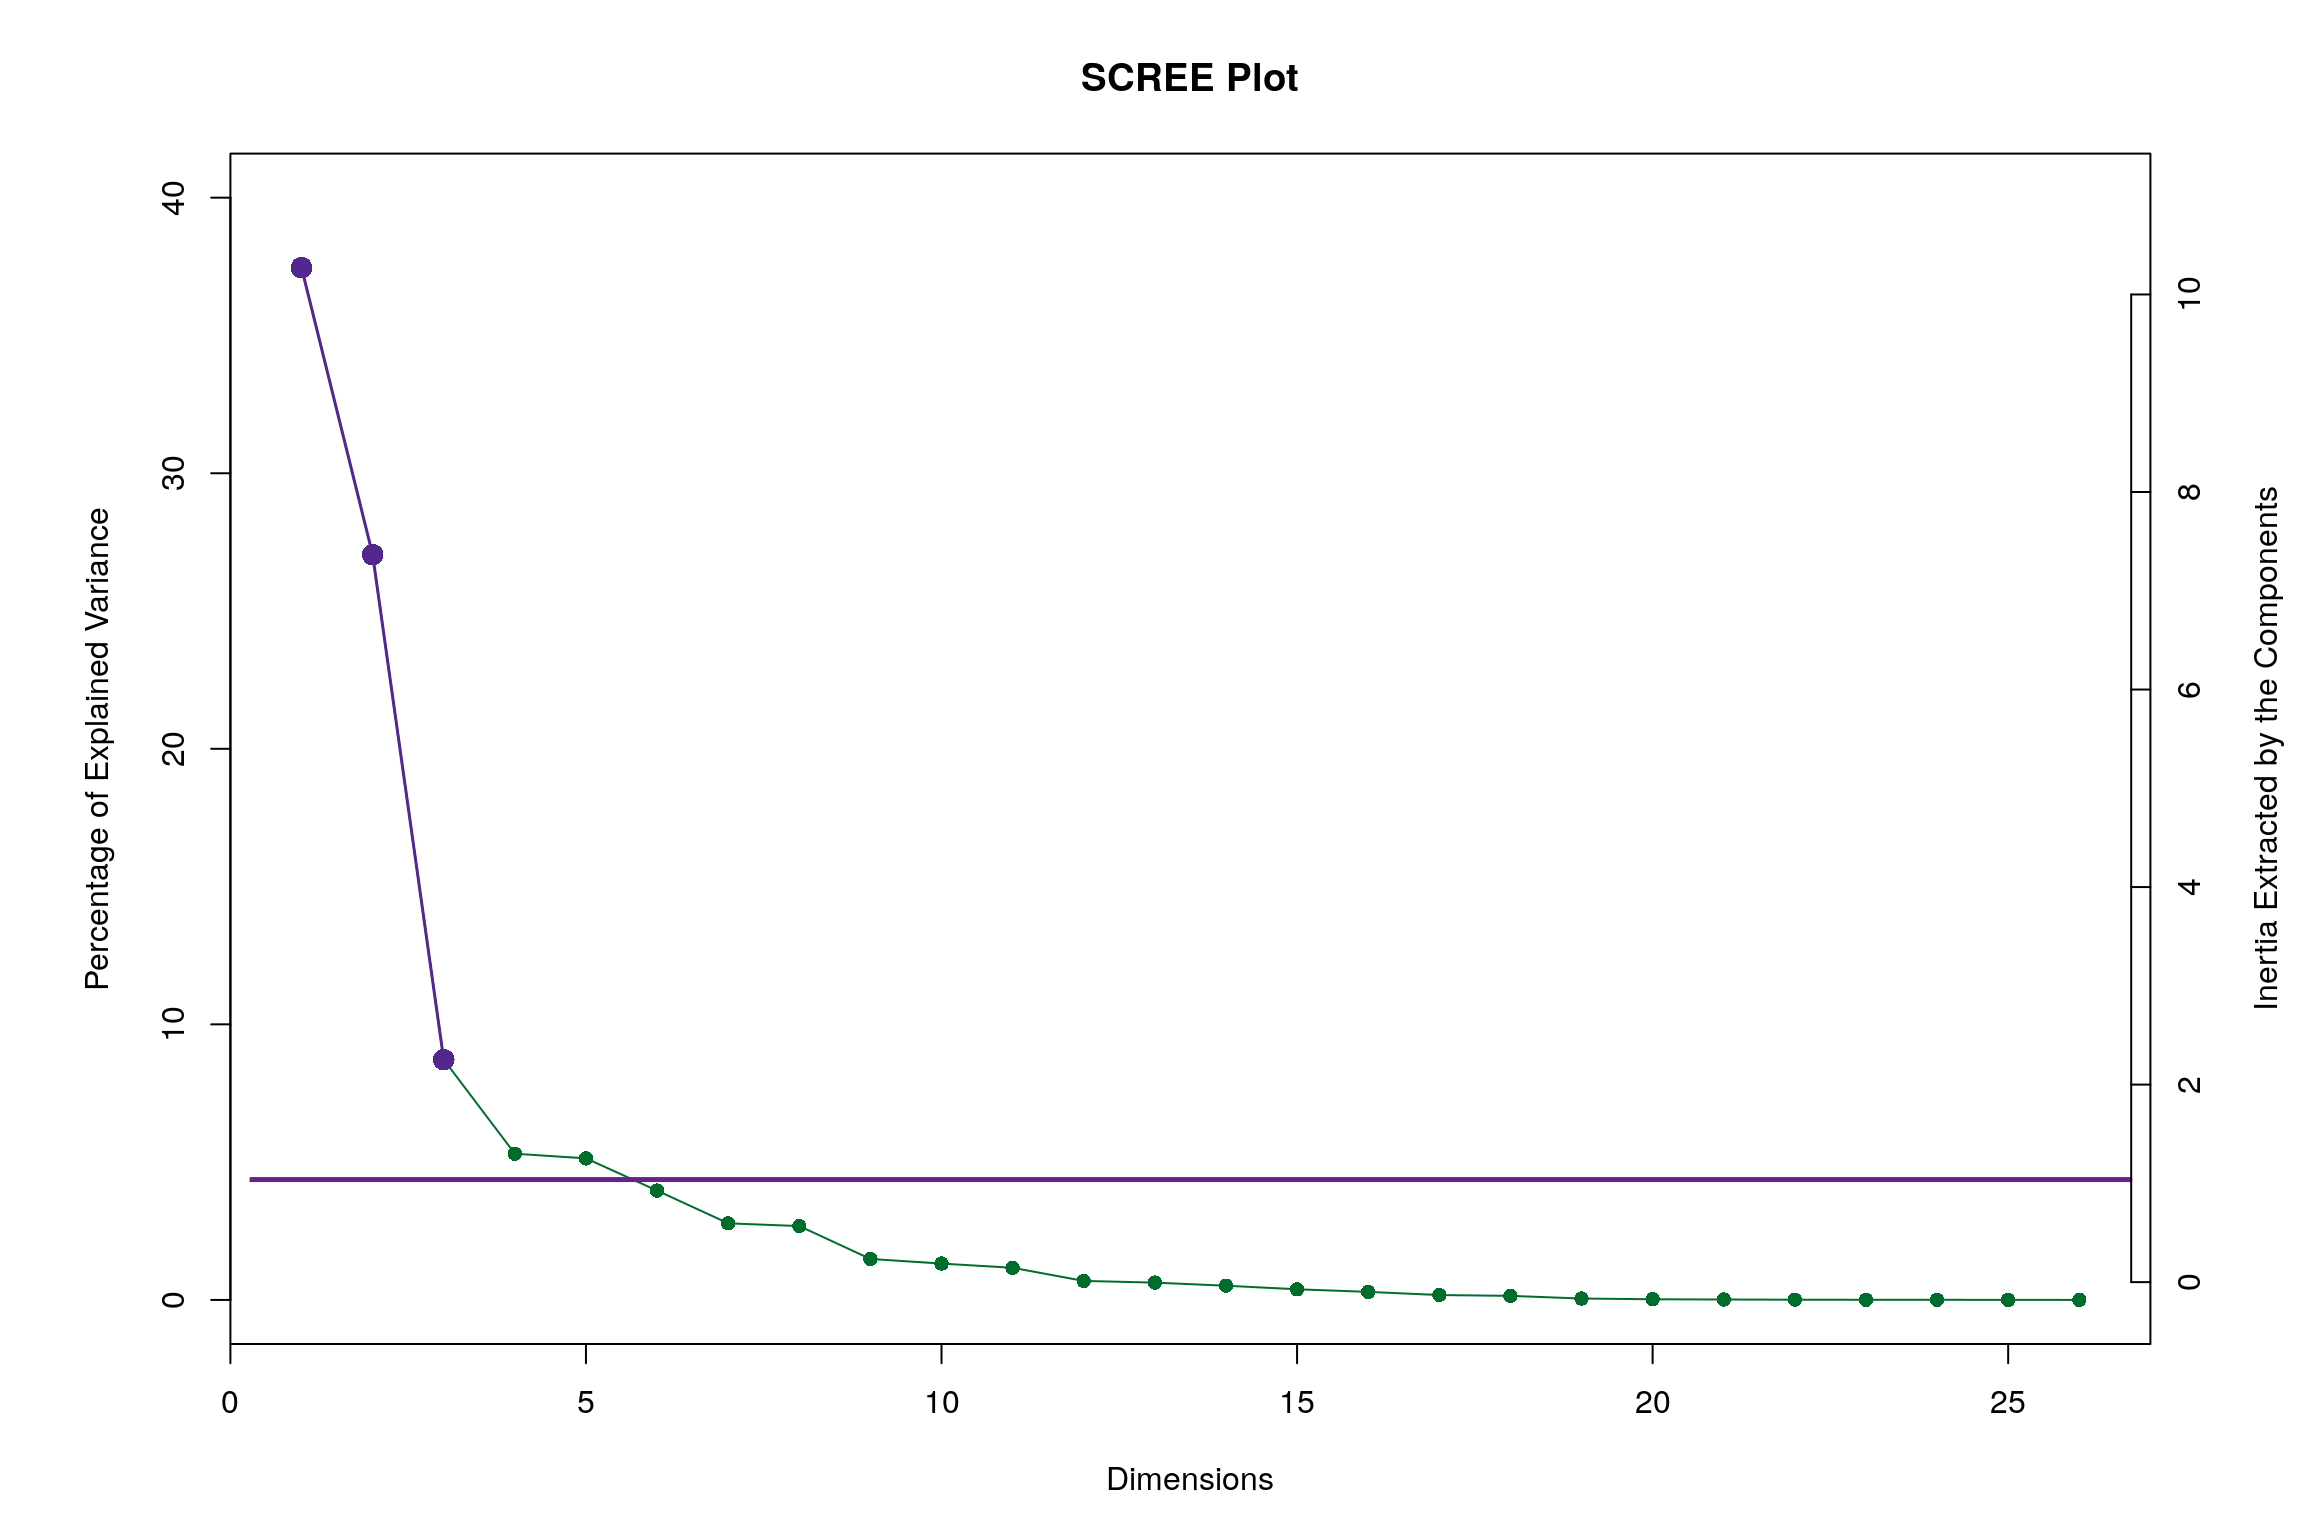
\includegraphics{Group1_Ritesh_Malaiya_PCA_Inference_World_env_vars_files/figure-latex/unnamed-chunk-7-1.pdf}
\includegraphics{Group1_Ritesh_Malaiya_PCA_Inference_World_env_vars_files/figure-latex/unnamed-chunk-7-2.pdf}
\includegraphics{Group1_Ritesh_Malaiya_PCA_Inference_World_env_vars_files/figure-latex/unnamed-chunk-7-3.pdf}
\includegraphics{Group1_Ritesh_Malaiya_PCA_Inference_World_env_vars_files/figure-latex/unnamed-chunk-7-4.pdf}
\includegraphics{Group1_Ritesh_Malaiya_PCA_Inference_World_env_vars_files/figure-latex/unnamed-chunk-7-5.pdf}

Since, it's not very straightforward to decide which components may be
best suited for the research question at hand, let's represent, in a
tabular format, which component helps to differentiate between which
design variable values (Happy, Happier, Happiest)

P.S. here -1 represents -ve quadrant of the component and +1 represent
+ve quadrant. 0 represents that component was not decisive enough to
clearly seperate happiness levels.

\begin{verbatim}
##              happy happier happiest
## Component 1     -1       1        0
## Component 2     -1       0        1
## Component 3      1       0       -1
## Component 4      0       0        0
## Component 5      0       0        0
## Component 6      0       0        0
## Component 7      1      -1        0
## Component 8      0       0        0
## Component 9      0      -1        1
## Component 10     0       0        0
\end{verbatim}

Looking at the table, it seems component 1, 2, 7, 9 may be able to best
represent all 3 happiness levels. Hence, let's plot components 1 vs 2
and 7 vs 9. Similarily, we will also plot Loading plots for these
componenets.

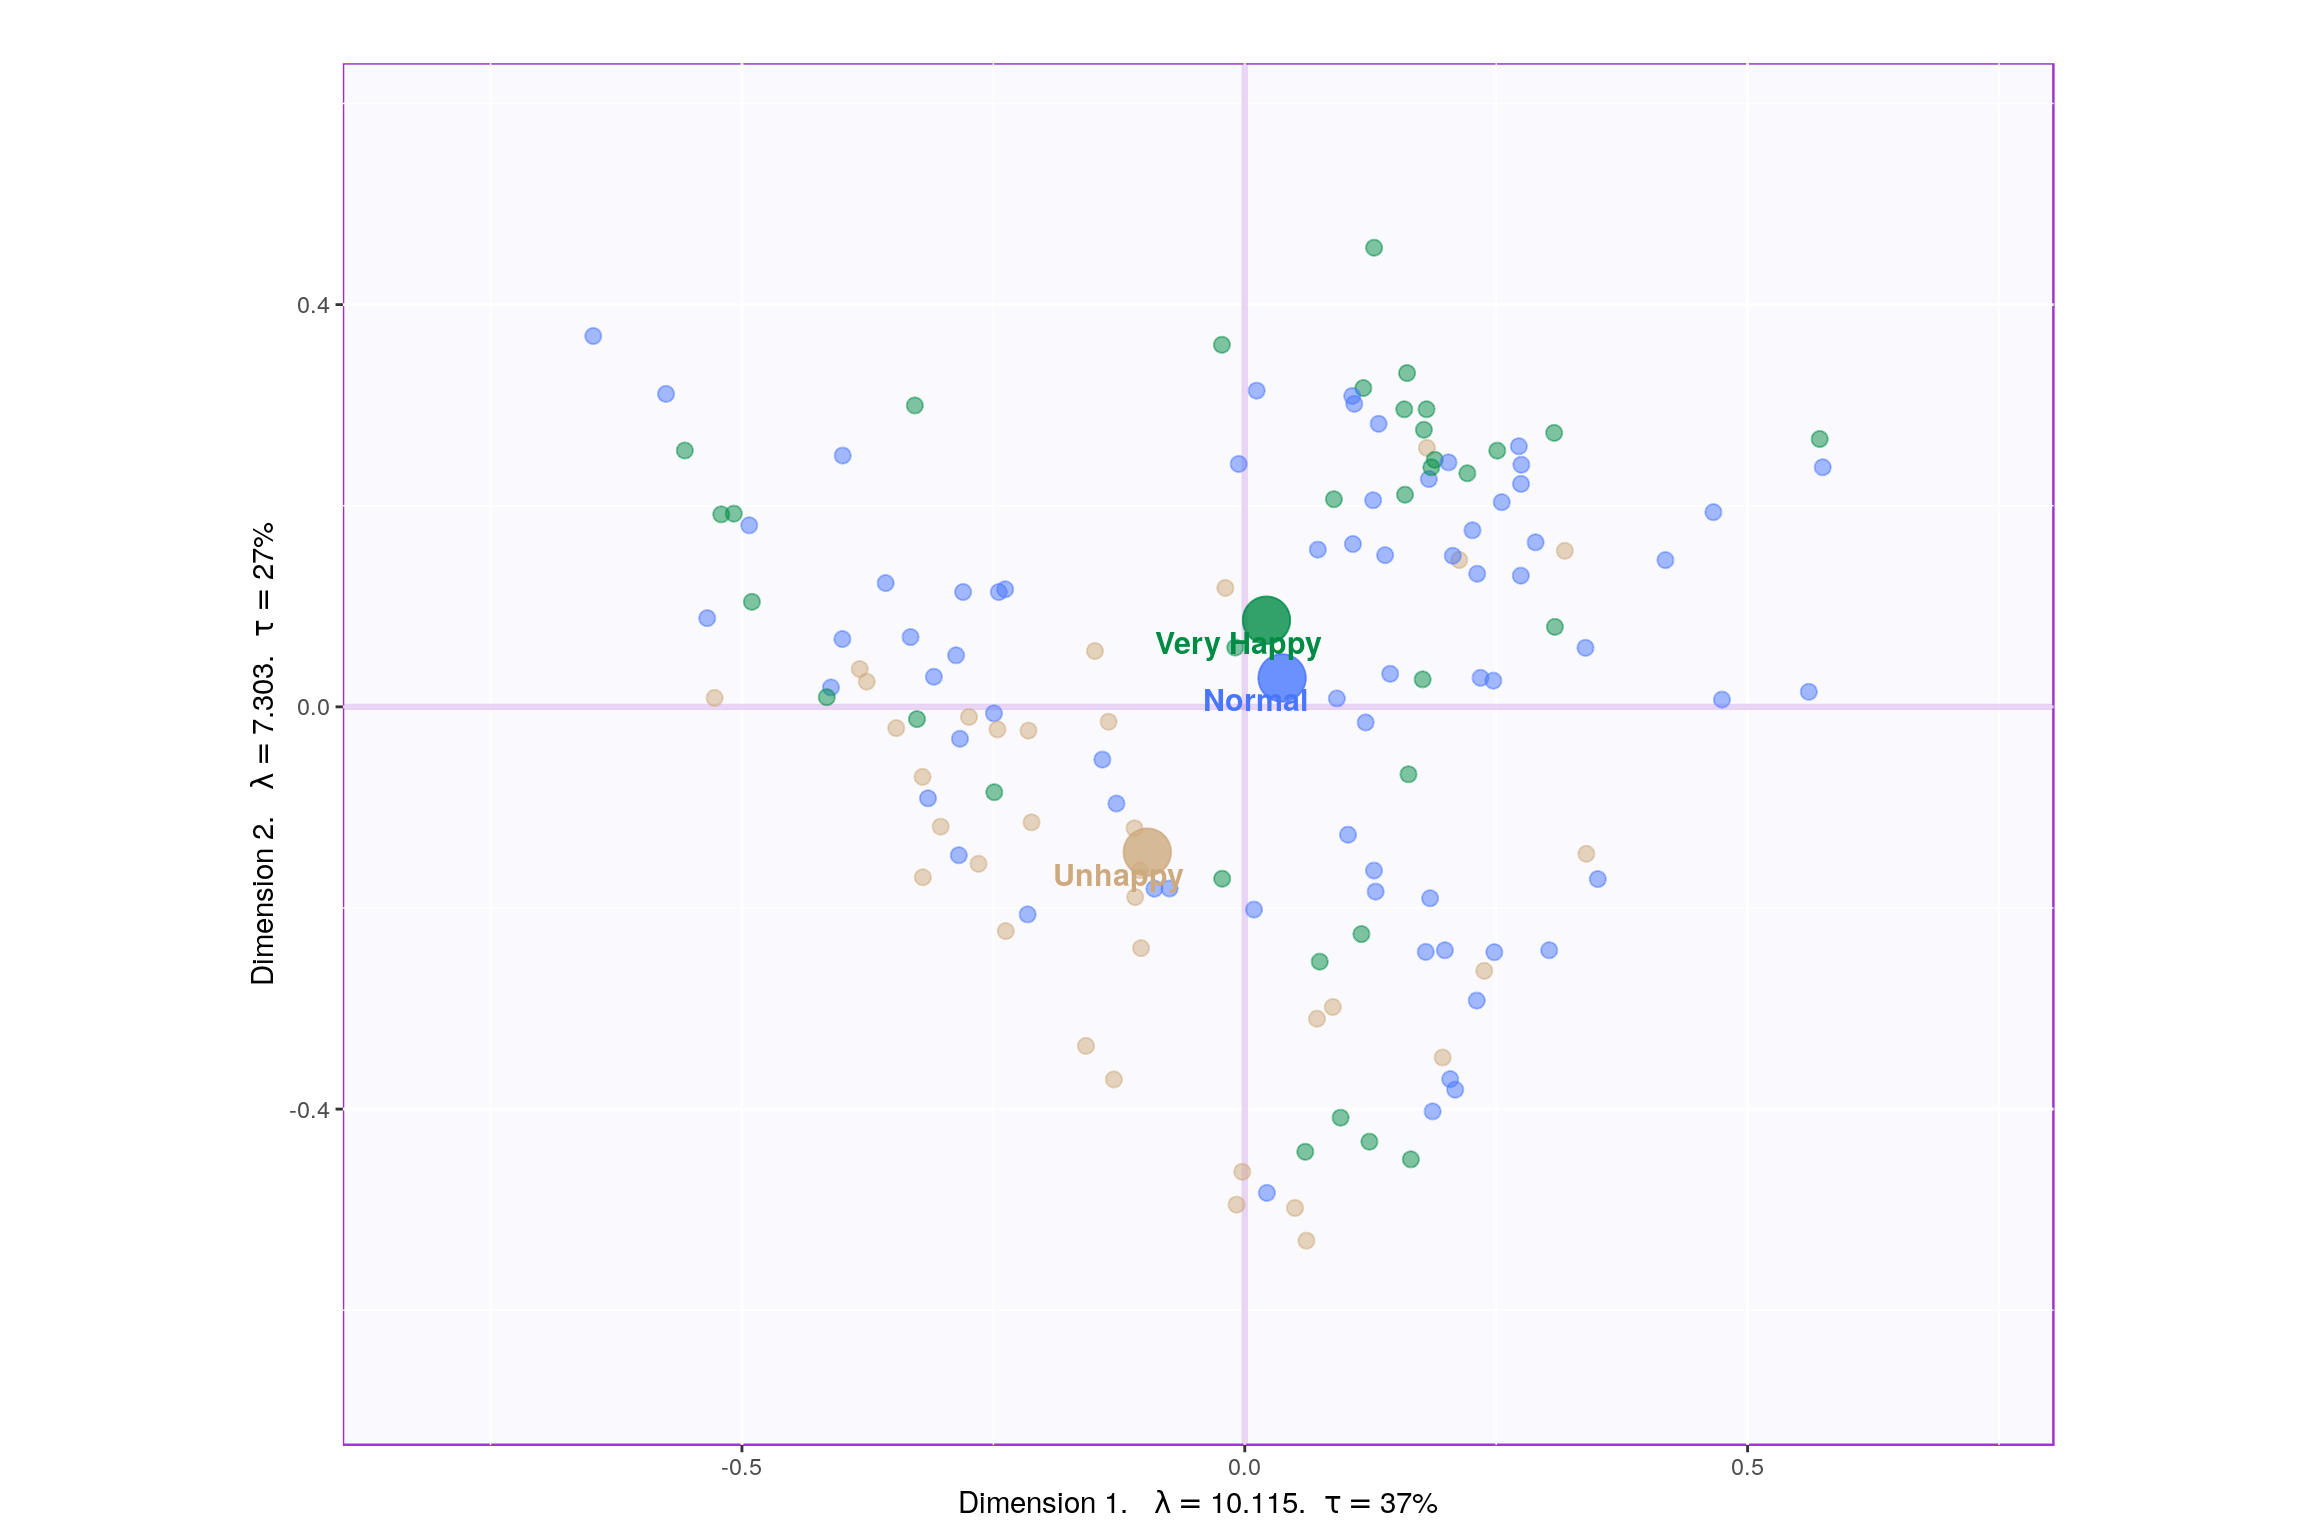
\includegraphics{Group1_Ritesh_Malaiya_PCA_Inference_World_env_vars_files/figure-latex/unnamed-chunk-9-1.pdf}
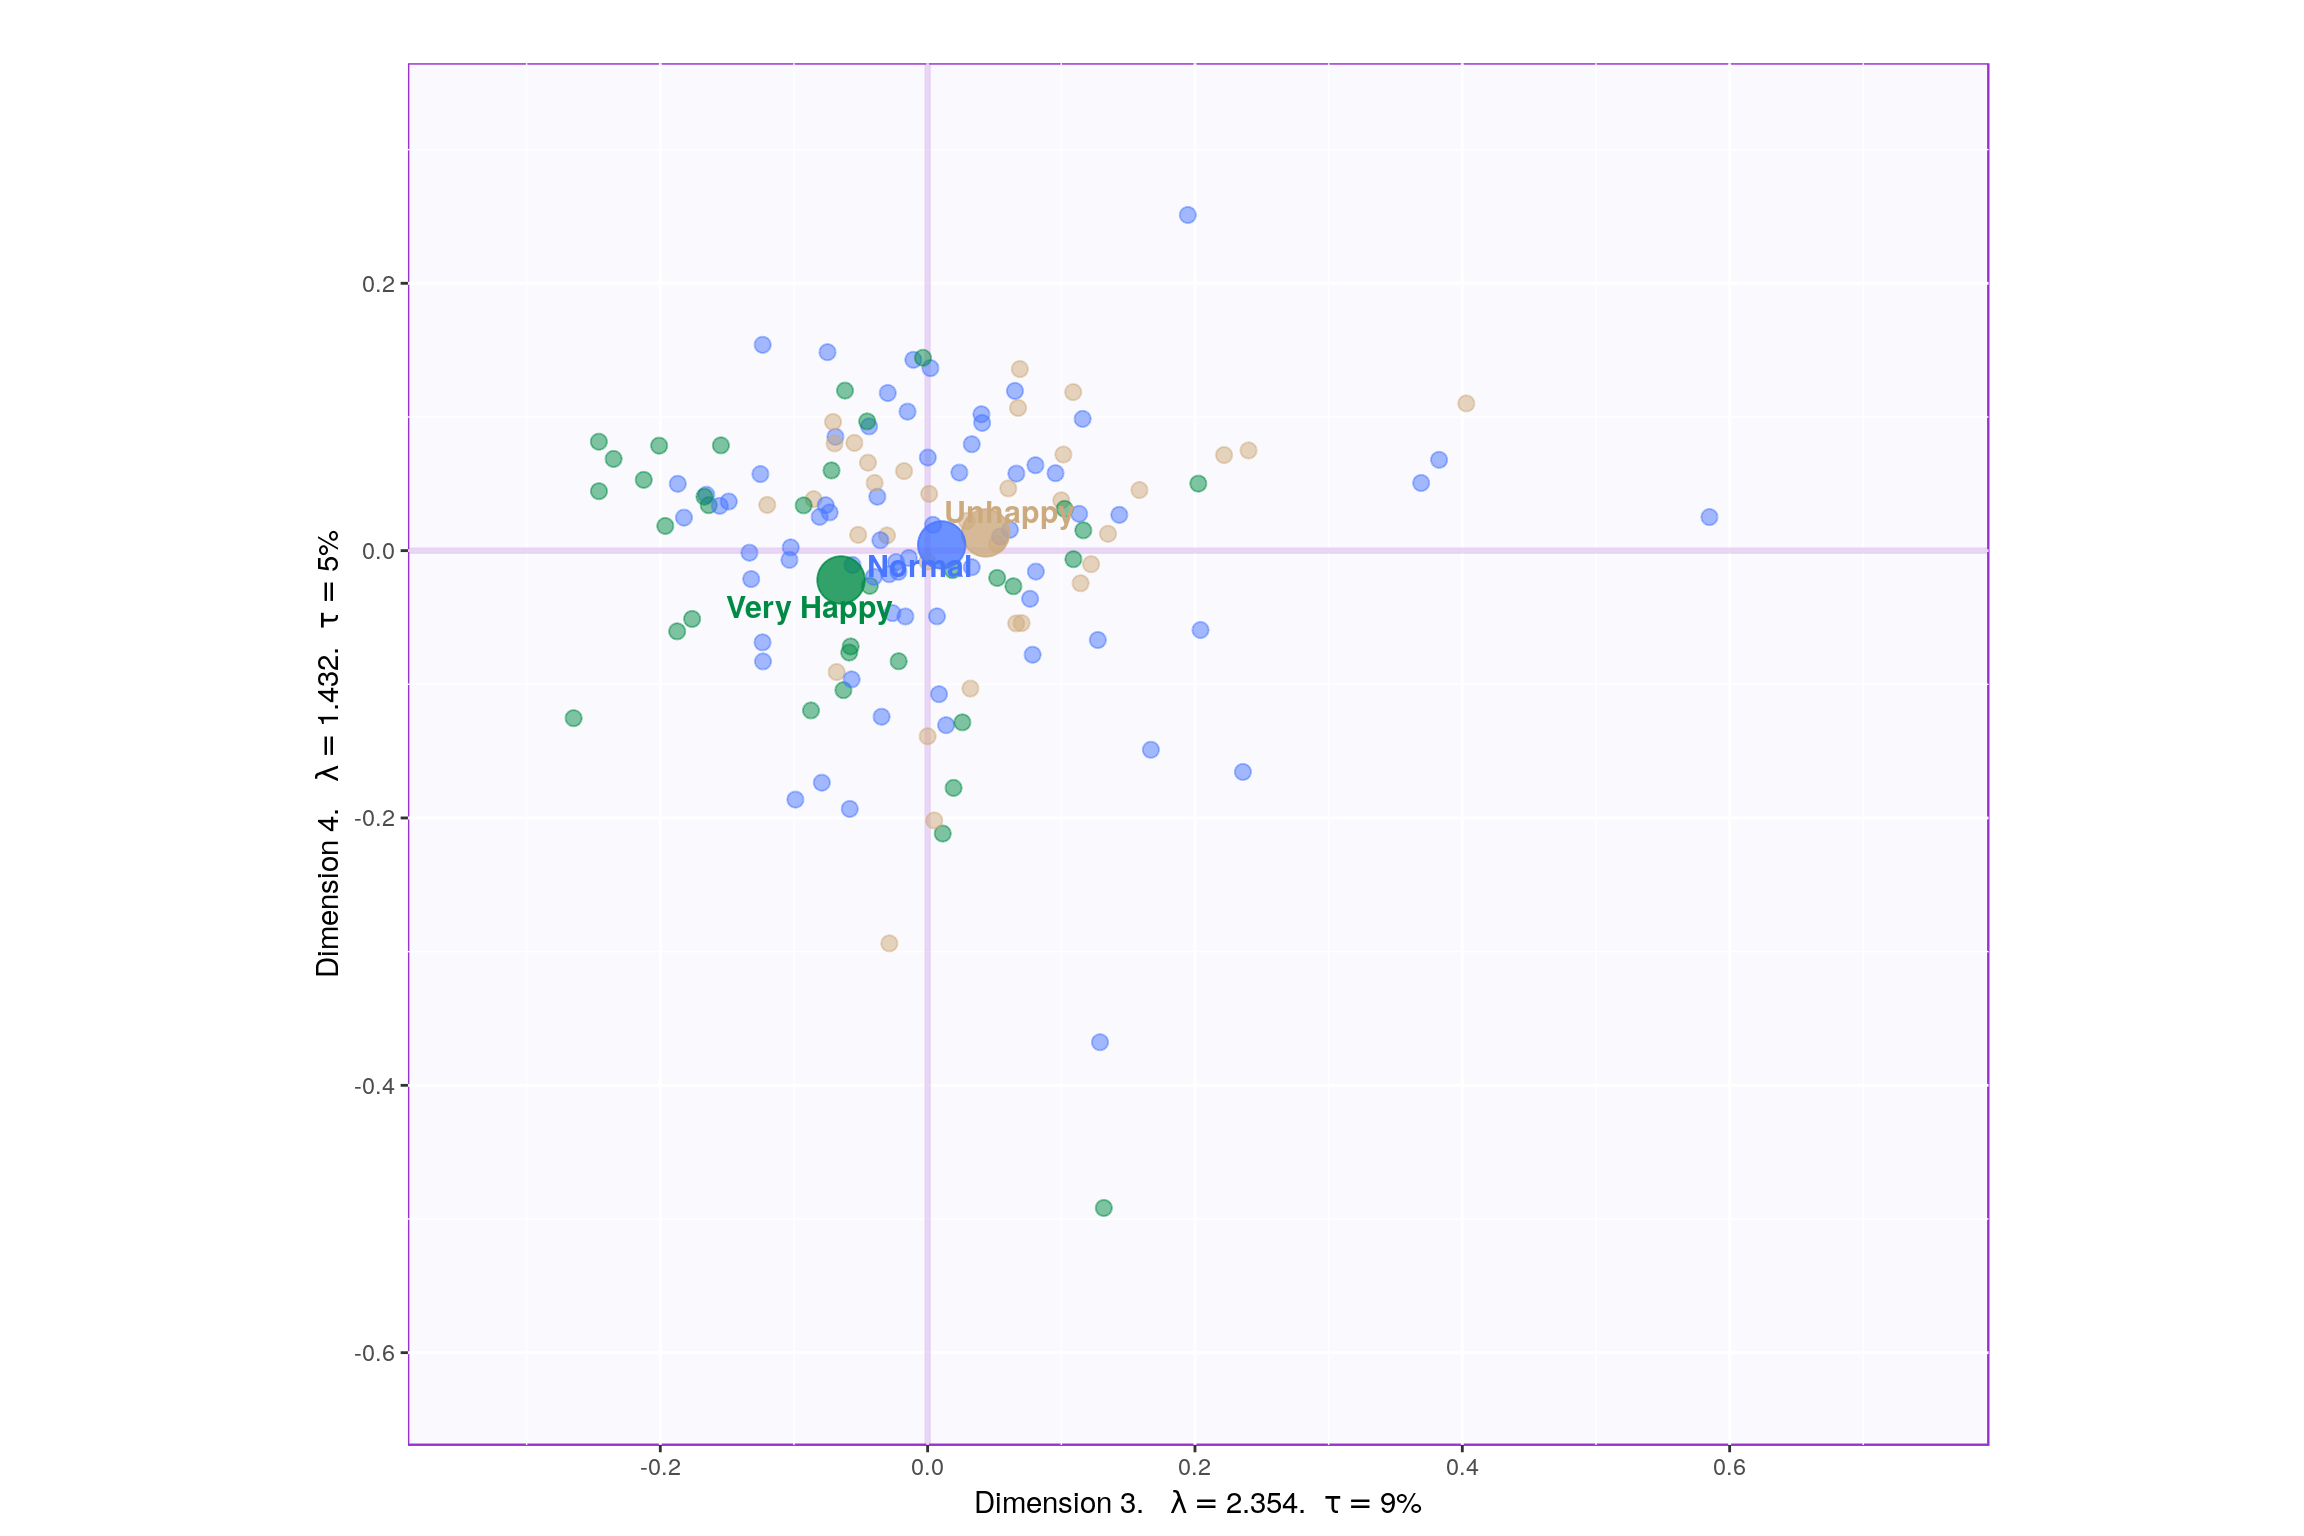
\includegraphics{Group1_Ritesh_Malaiya_PCA_Inference_World_env_vars_files/figure-latex/unnamed-chunk-9-2.pdf}

\hypertarget{loadings}{%
\paragraph{Loadings}\label{loadings}}

\begin{Shaded}
\begin{Highlighting}[]
\ControlFlowTok{for}\NormalTok{ (i }\ControlFlowTok{in} \DecValTok{1}\OperatorTok{:}\DecValTok{2}\NormalTok{)\{}
  
\NormalTok{  axis1 =}\StringTok{ }\NormalTok{loop[i,}\DecValTok{1}\NormalTok{]}
\NormalTok{  axis2 =}\StringTok{ }\NormalTok{loop[i,}\DecValTok{2}\NormalTok{]}

\NormalTok{  col_palate =}\StringTok{ }\KeywordTok{brewer.pal}\NormalTok{(}\DataTypeTok{n =} \DecValTok{12}\NormalTok{, }\DataTypeTok{name=}\StringTok{'Set3'}\NormalTok{)}
  
\NormalTok{  col4J =}\StringTok{ }\KeywordTok{vector}\NormalTok{(}\StringTok{'list'}\NormalTok{, }\KeywordTok{nrow}\NormalTok{(country_env_pca}\OperatorTok{$}\NormalTok{ExPosition.Data}\OperatorTok{$}\NormalTok{fj))}
\NormalTok{  col4J[}\KeywordTok{grep}\NormalTok{(}\StringTok{'rain'}\NormalTok{,}\KeywordTok{rownames}\NormalTok{(country_env_pca}\OperatorTok{$}\NormalTok{ExPosition.Data}\OperatorTok{$}\NormalTok{fj))] =}\StringTok{ }\NormalTok{col_palate[}\DecValTok{1}\NormalTok{]}
\NormalTok{  col4J[}\KeywordTok{grep}\NormalTok{(}\StringTok{'temp'}\NormalTok{,}\KeywordTok{rownames}\NormalTok{(country_env_pca}\OperatorTok{$}\NormalTok{ExPosition.Data}\OperatorTok{$}\NormalTok{fj))] =}\StringTok{ 'red'} \CommentTok{#col_palate[2]}
\NormalTok{  col4J[}\KeywordTok{sapply}\NormalTok{(col4J, }\StringTok{'is.null'}\NormalTok{)] =}\StringTok{ }\NormalTok{col_palate[}\DecValTok{3}\OperatorTok{:}\DecValTok{11}\NormalTok{]}
  
\NormalTok{  loadings_}\DecValTok{2}\NormalTok{ <-}\StringTok{ }\KeywordTok{cor}\NormalTok{(country_env_df_for_pca, country_env_pca}\OperatorTok{$}\NormalTok{ExPosition.Data}\OperatorTok{$}\NormalTok{fi)}
  
\NormalTok{  loadings_map <-}\StringTok{ }\NormalTok{PTCA4CATA}\OperatorTok{::}\KeywordTok{createFactorMap}\NormalTok{(loadings_}\DecValTok{2}\NormalTok{, }
                          \DataTypeTok{col.points =}\NormalTok{ col4J, }
                          \DataTypeTok{col.labels =}\NormalTok{ col4J, }
                          \DataTypeTok{axis1=}\NormalTok{axis1,}
                          \DataTypeTok{axis2=}\NormalTok{axis2,}
                          \DataTypeTok{constraints =} \KeywordTok{list}\NormalTok{(}\DataTypeTok{minx =} \DecValTok{-1}\NormalTok{, }\DataTypeTok{miny =} \DecValTok{-1}\NormalTok{, }\DataTypeTok{maxx =} \DecValTok{1}\NormalTok{ , }\DataTypeTok{maxy =} \DecValTok{1}\NormalTok{)) }
  
\NormalTok{  country_label4Map <-}\StringTok{ }\NormalTok{PTCA4CATA}\OperatorTok{::}\KeywordTok{createxyLabels.gen}\NormalTok{(axis1,axis2,}\DataTypeTok{lambda =}\NormalTok{ country_env_pca}\OperatorTok{$}\NormalTok{ExPosition.Data}\OperatorTok{$}\NormalTok{eigs, }\DataTypeTok{tau =}\NormalTok{ country_env_pca}\OperatorTok{$}\NormalTok{ExPosition.Data}\OperatorTok{$}\NormalTok{t) }
  
\NormalTok{  corr_map <-}\StringTok{ }\NormalTok{loadings_map}\OperatorTok{$}\NormalTok{zeMap_background  }\OperatorTok{+}\StringTok{  }\NormalTok{country_label4Map }\OperatorTok{+}\StringTok{ }\NormalTok{PTCA4CATA}\OperatorTok{::}\KeywordTok{addCircleOfCor}\NormalTok{() }\OperatorTok{+}
\StringTok{              }\NormalTok{loadings_map}\OperatorTok{$}\NormalTok{zeMap_text }\OperatorTok{+}
\StringTok{              }\NormalTok{PTCA4CATA}\OperatorTok{::}\KeywordTok{addArrows}\NormalTok{(loadings_}\DecValTok{2}\NormalTok{, }\DataTypeTok{color =}\NormalTok{ col4J) }
  
  \KeywordTok{print}\NormalTok{(corr_map)}
\NormalTok{\}}
\end{Highlighting}
\end{Shaded}

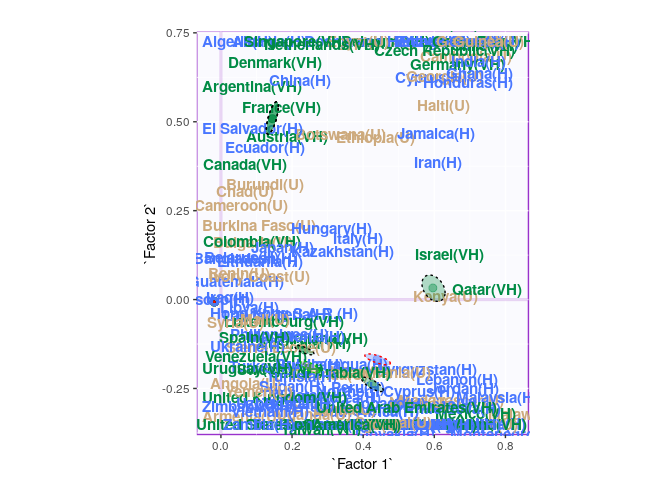
\includegraphics{Group1_Ritesh_Malaiya_PCA_Inference_World_env_vars_files/figure-latex/unnamed-chunk-10-1.pdf}
\includegraphics{Group1_Ritesh_Malaiya_PCA_Inference_World_env_vars_files/figure-latex/unnamed-chunk-10-2.pdf}

Rain, compared with Temperature, cloudiness and tree coverage seems to
be almost orthogonal to each other, hence are \emph{not} correlated.

\hypertarget{most-contributing-variables}{%
\paragraph{Most Contributing
Variables}\label{most-contributing-variables}}

Let's plot variable contributions against each chosen components i.e.~1,
7, 9.

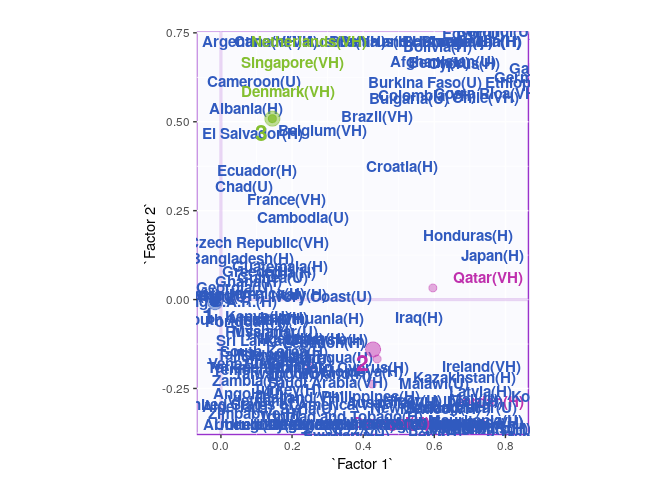
\includegraphics{Group1_Ritesh_Malaiya_PCA_Inference_World_env_vars_files/figure-latex/unnamed-chunk-11-1.pdf}
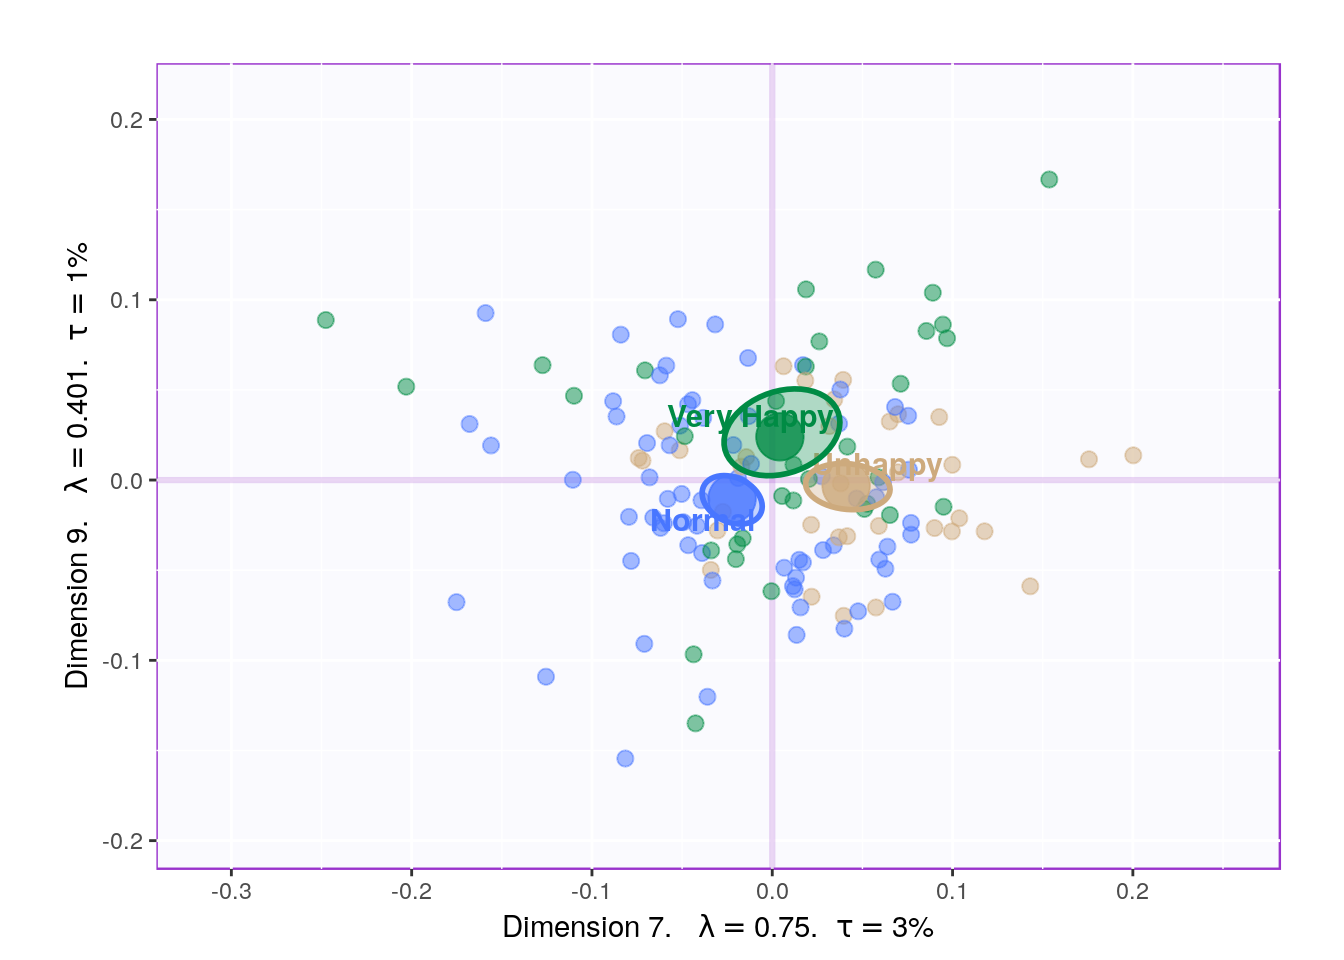
\includegraphics{Group1_Ritesh_Malaiya_PCA_Inference_World_env_vars_files/figure-latex/unnamed-chunk-11-2.pdf}
\includegraphics{Group1_Ritesh_Malaiya_PCA_Inference_World_env_vars_files/figure-latex/unnamed-chunk-11-3.pdf}
\includegraphics{Group1_Ritesh_Malaiya_PCA_Inference_World_env_vars_files/figure-latex/unnamed-chunk-11-4.pdf}

\hypertarget{inference-pca}{%
\subsubsection{Inference PCA}\label{inference-pca}}

\begin{verbatim}
## [1] "It is estimated that your iterations will take 0.02 minutes."
## [1] "R is not in interactive() mode. Resample-based tests will be conducted. Please take note of the progress bar."
## ===========================================================================
\end{verbatim}

\hypertarget{scree-plot-with-inference}{%
\paragraph{Scree Plot (with
Inference)}\label{scree-plot-with-inference}}

\begin{Shaded}
\begin{Highlighting}[]
\NormalTok{PTCA4CATA}\OperatorTok{::}\KeywordTok{PlotScree}\NormalTok{(}\DataTypeTok{ev =}\NormalTok{ country_env_pca}\OperatorTok{$}\NormalTok{ExPosition.Data}\OperatorTok{$}\NormalTok{eigs,}
                      \DataTypeTok{p.ev =}\NormalTok{  country_env_pca_inf}\OperatorTok{$}\NormalTok{Inference.Data}\OperatorTok{$}\NormalTok{components}\OperatorTok{$}\NormalTok{p.vals,}
                      \DataTypeTok{title =} \StringTok{'Eigenvalues Inference'}\NormalTok{,}
                      \DataTypeTok{plotKaiser =} \OtherTok{TRUE}
\NormalTok{)}
\end{Highlighting}
\end{Shaded}

\includegraphics{Group1_Ritesh_Malaiya_PCA_Inference_World_env_vars_files/figure-latex/scree_inf-1.pdf}

Although, this plot suggests that \(3^{rd}\) and \(4^{th}\) components
might be useful, from our above analysis we know that otherwise. Also,
this plot suggests that component \(6^{th}\) and onwards might not be
useful which is contradicting our findings above.

\hypertarget{permutation-test}{%
\paragraph{Permutation Test}\label{permutation-test}}

\begin{Shaded}
\begin{Highlighting}[]
\ControlFlowTok{for}\NormalTok{ (i }\ControlFlowTok{in} \KeywordTok{c}\NormalTok{(}\DecValTok{1}\NormalTok{, }\DecValTok{2}\NormalTok{, }\DecValTok{7}\NormalTok{, }\DecValTok{9}\NormalTok{)) \{}
\NormalTok{zeDim =}\StringTok{ }\NormalTok{i}
\NormalTok{pH1 <-}\StringTok{ }\KeywordTok{prettyHist}\NormalTok{(}
  \DataTypeTok{distribution =}\NormalTok{ country_env_pca_inf}\OperatorTok{$}\NormalTok{Inference.Data}\OperatorTok{$}\NormalTok{components}\OperatorTok{$}\NormalTok{eigs.perm[,zeDim], }
  \DataTypeTok{observed =}\NormalTok{ country_env_pca_inf}\OperatorTok{$}\NormalTok{Fixed.Data}\OperatorTok{$}\NormalTok{ExPosition.Data}\OperatorTok{$}\NormalTok{eigs[zeDim], }
  \DataTypeTok{xlim =} \KeywordTok{c}\NormalTok{(}\DecValTok{0}\NormalTok{, }\FloatTok{4.5}\NormalTok{), }\CommentTok{# needs to be set by hand}
  \DataTypeTok{breaks =} \DecValTok{20}\NormalTok{,}
  \DataTypeTok{border =} \StringTok{"white"}\NormalTok{, }
  \DataTypeTok{main =} \KeywordTok{paste0}\NormalTok{(}\StringTok{"Permutation Test for Eigenvalue "}\NormalTok{,zeDim),}
  \DataTypeTok{xlab =} \KeywordTok{paste0}\NormalTok{(}\StringTok{"Eigenvalue "}\NormalTok{,zeDim), }
  \DataTypeTok{ylab =} \StringTok{""}\NormalTok{, }
  \DataTypeTok{counts =} \OtherTok{FALSE}\NormalTok{, }
  \DataTypeTok{cutoffs =} \KeywordTok{c}\NormalTok{( }\FloatTok{0.975}\NormalTok{))}
\NormalTok{\}}
\end{Highlighting}
\end{Shaded}

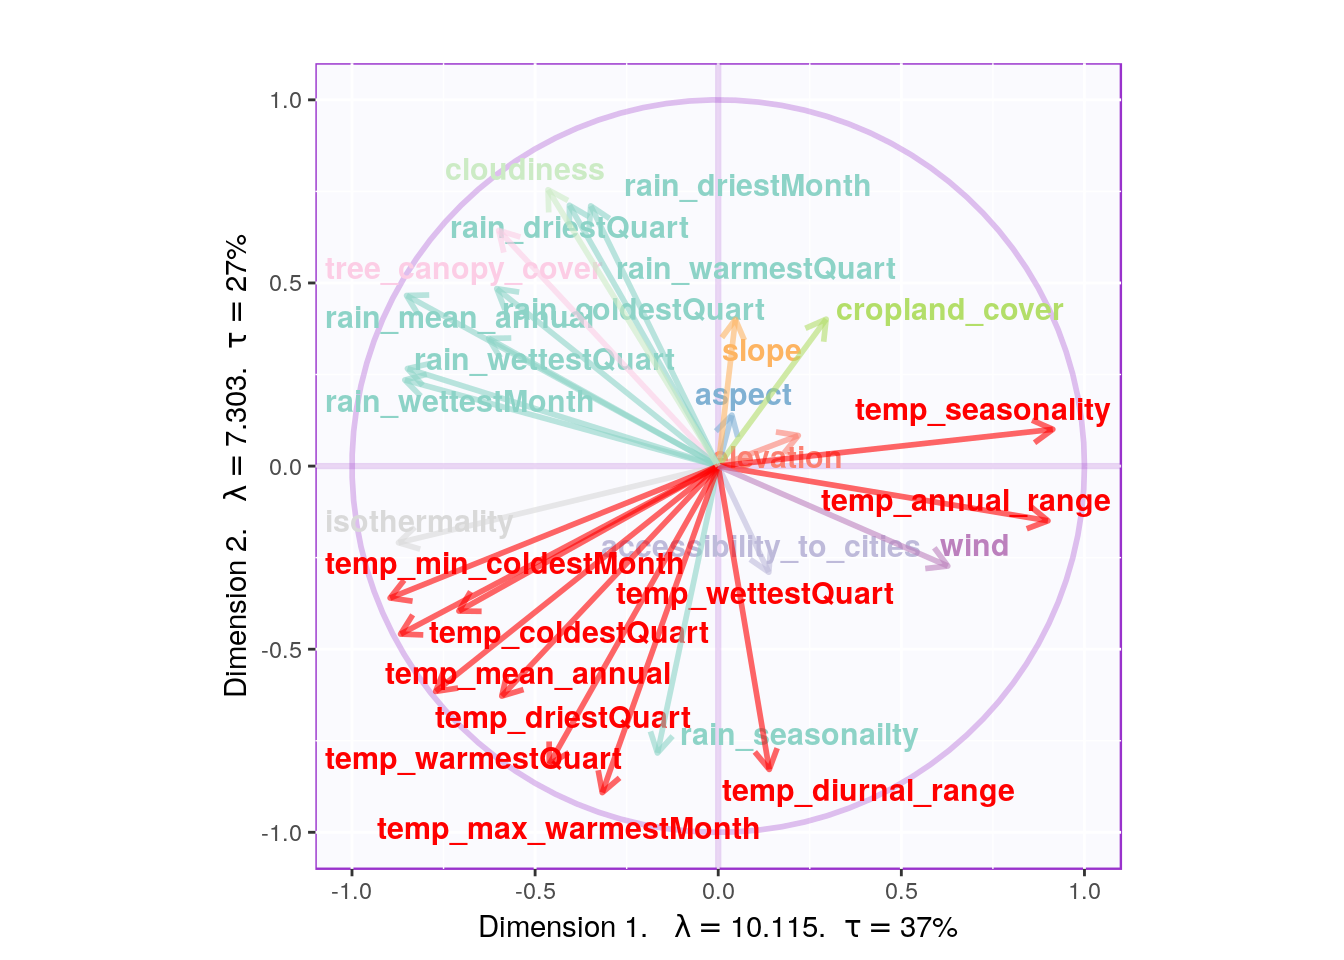
\includegraphics{Group1_Ritesh_Malaiya_PCA_Inference_World_env_vars_files/figure-latex/unnamed-chunk-13-1.pdf}
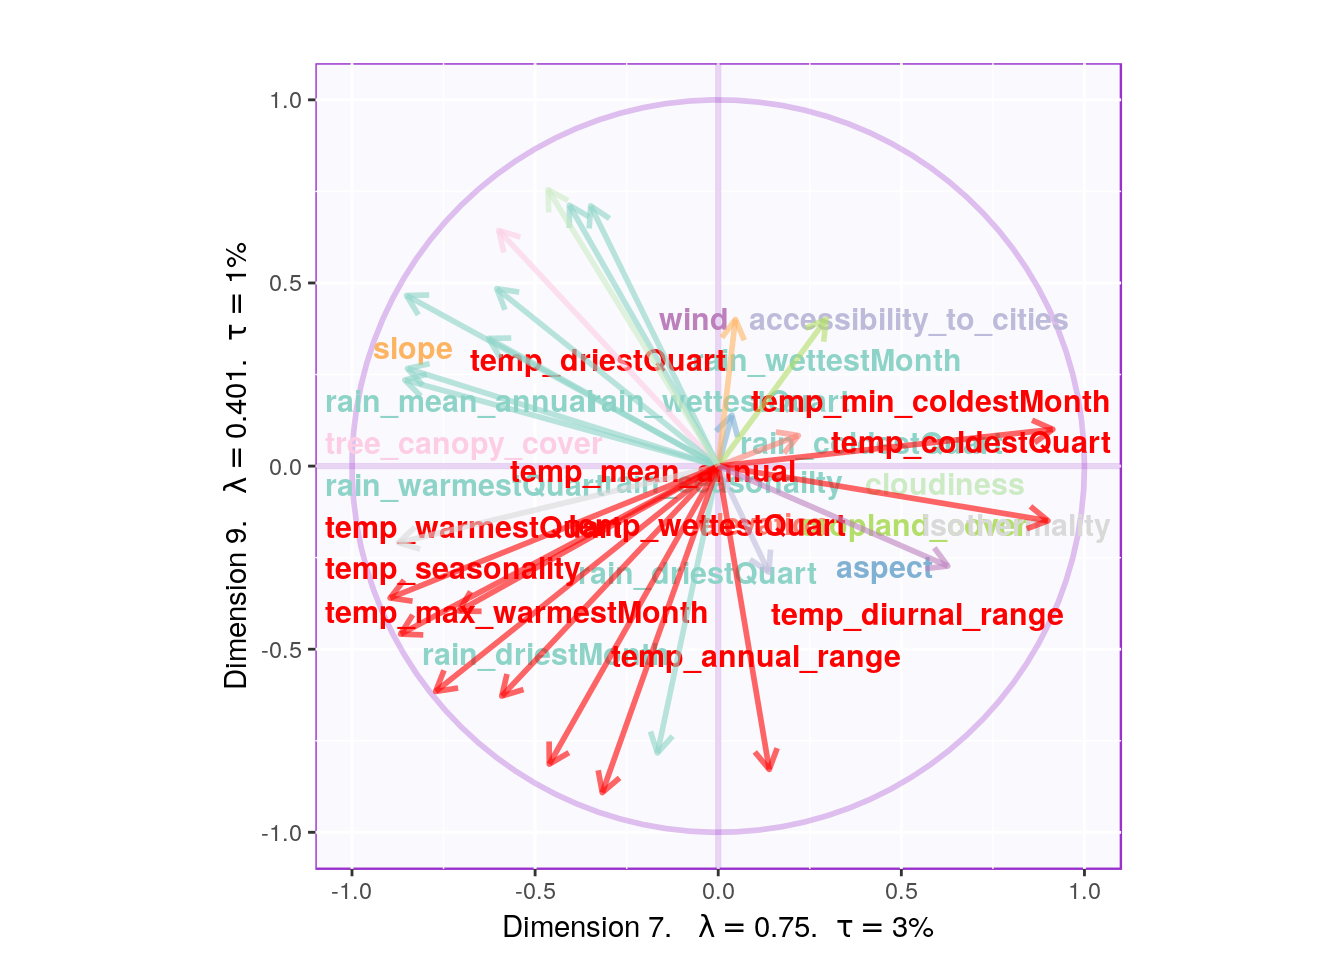
\includegraphics{Group1_Ritesh_Malaiya_PCA_Inference_World_env_vars_files/figure-latex/unnamed-chunk-13-2.pdf}
\includegraphics{Group1_Ritesh_Malaiya_PCA_Inference_World_env_vars_files/figure-latex/unnamed-chunk-13-3.pdf}
\includegraphics{Group1_Ritesh_Malaiya_PCA_Inference_World_env_vars_files/figure-latex/unnamed-chunk-13-4.pdf}

\hypertarget{parallet-test}{%
\paragraph{Parallet Test}\label{parallet-test}}

\begin{Shaded}
\begin{Highlighting}[]
\NormalTok{country_env_pca_mc <-}\StringTok{ }\NormalTok{data4PCCAR}\OperatorTok{::}\KeywordTok{monteCarlo.eigen}\NormalTok{(}\DataTypeTok{X =}\NormalTok{ country_env_df_for_pca, }\DataTypeTok{nIter =} \DecValTok{10000}\NormalTok{)}
\ControlFlowTok{for}\NormalTok{ (i }\ControlFlowTok{in} \KeywordTok{c}\NormalTok{(}\DecValTok{1}\NormalTok{, }\DecValTok{2}\NormalTok{, }\DecValTok{7}\NormalTok{, }\DecValTok{9}\NormalTok{)) \{}
\NormalTok{  zeDim =}\StringTok{ }\NormalTok{i}
\NormalTok{  pH1.p <-}\StringTok{ }\KeywordTok{prettyHist}\NormalTok{(country_env_pca_mc}\OperatorTok{$}\NormalTok{rand.eigs[,zeDim], }
                    \DataTypeTok{observed =}\NormalTok{ country_env_pca_mc}\OperatorTok{$}\NormalTok{fixed.eigs[zeDim], }
                    \DataTypeTok{xlim =} \KeywordTok{c}\NormalTok{(}\DecValTok{0}\NormalTok{, }\FloatTok{4.5}\NormalTok{), }\CommentTok{# needs to set by hand}
                    \DataTypeTok{breaks =} \DecValTok{20}\NormalTok{,}
                    \DataTypeTok{border =} \StringTok{"white"}\NormalTok{, }
                    \DataTypeTok{main =} \KeywordTok{paste0}\NormalTok{(}\StringTok{"Monte Carlo (Parallel) Test for Eigenvalue "}\NormalTok{,zeDim),}
                    \DataTypeTok{xlab =} \KeywordTok{paste0}\NormalTok{(}\StringTok{"Eigenvalue "}\NormalTok{,zeDim), }
                    \DataTypeTok{ylab =} \StringTok{""}\NormalTok{, }
                    \DataTypeTok{counts =} \OtherTok{FALSE}\NormalTok{, }
                    \DataTypeTok{cutoffs =} \KeywordTok{c}\NormalTok{( }\FloatTok{0.975}\NormalTok{))}
\NormalTok{\}}
\end{Highlighting}
\end{Shaded}

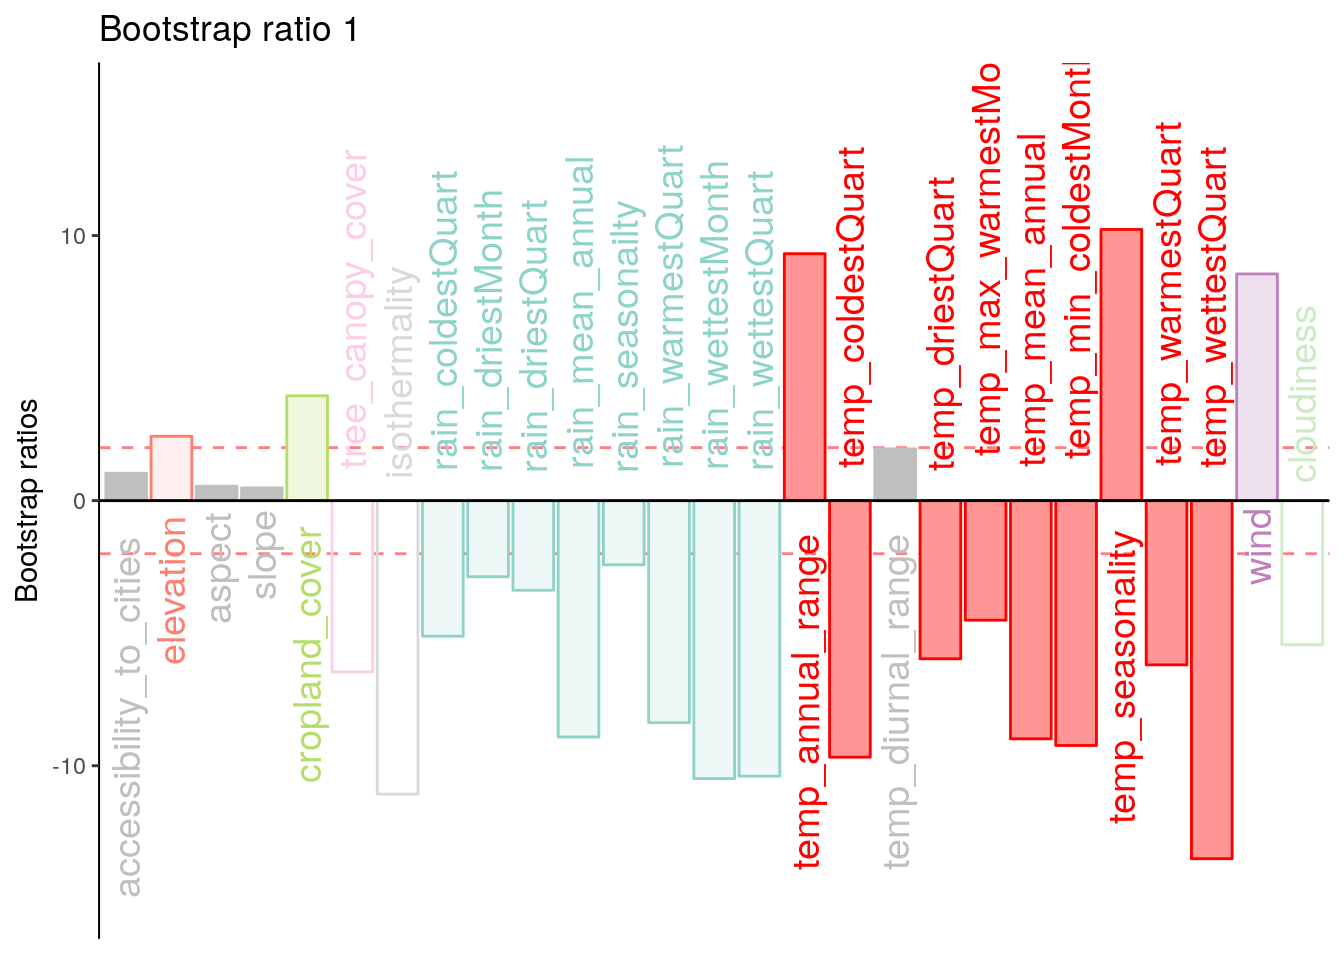
\includegraphics{Group1_Ritesh_Malaiya_PCA_Inference_World_env_vars_files/figure-latex/unnamed-chunk-14-1.pdf}
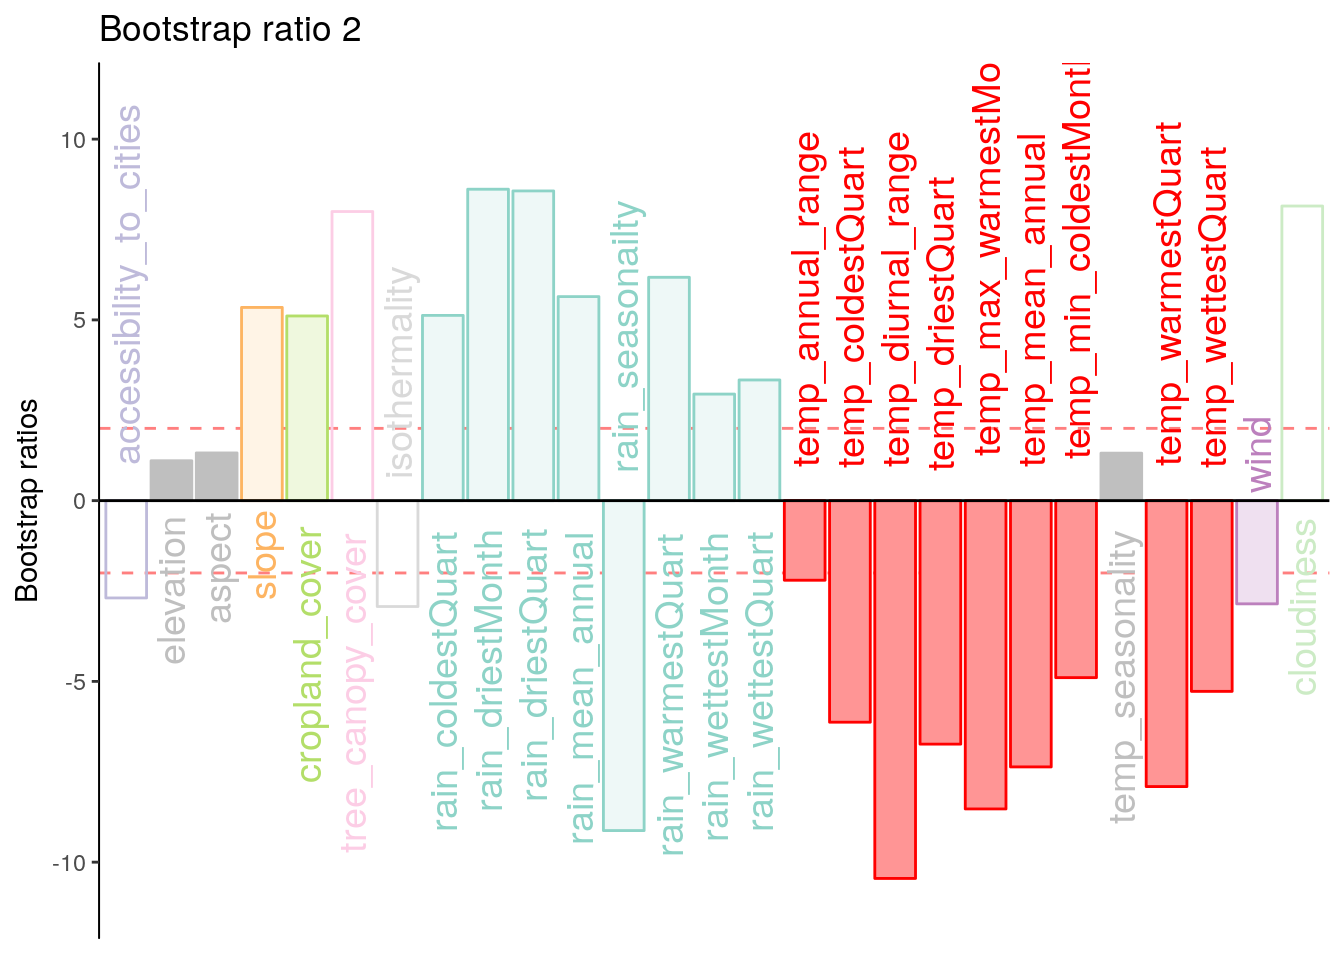
\includegraphics{Group1_Ritesh_Malaiya_PCA_Inference_World_env_vars_files/figure-latex/unnamed-chunk-14-2.pdf}
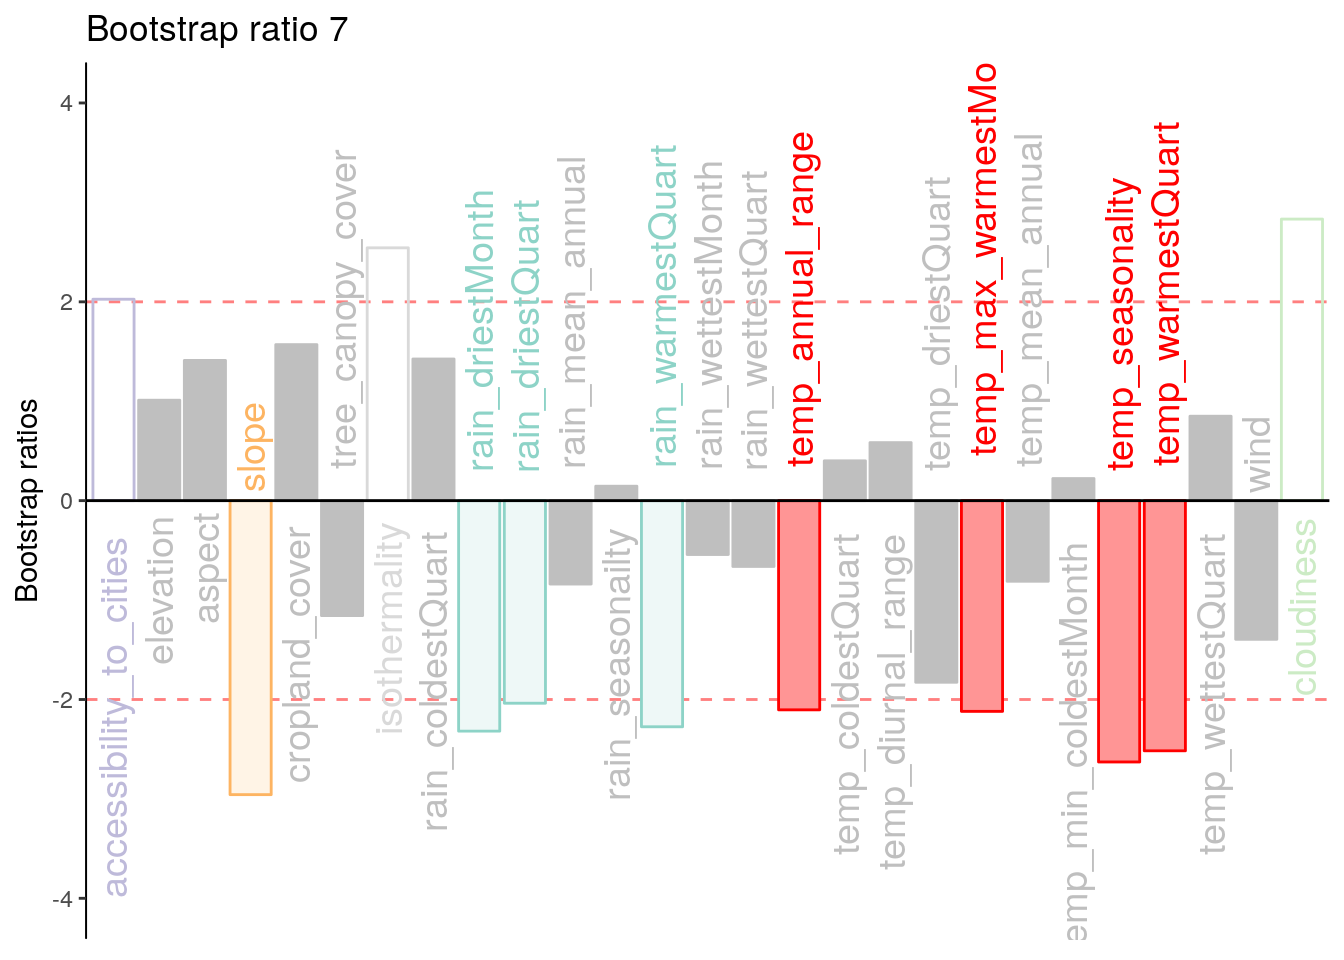
\includegraphics{Group1_Ritesh_Malaiya_PCA_Inference_World_env_vars_files/figure-latex/unnamed-chunk-14-3.pdf}
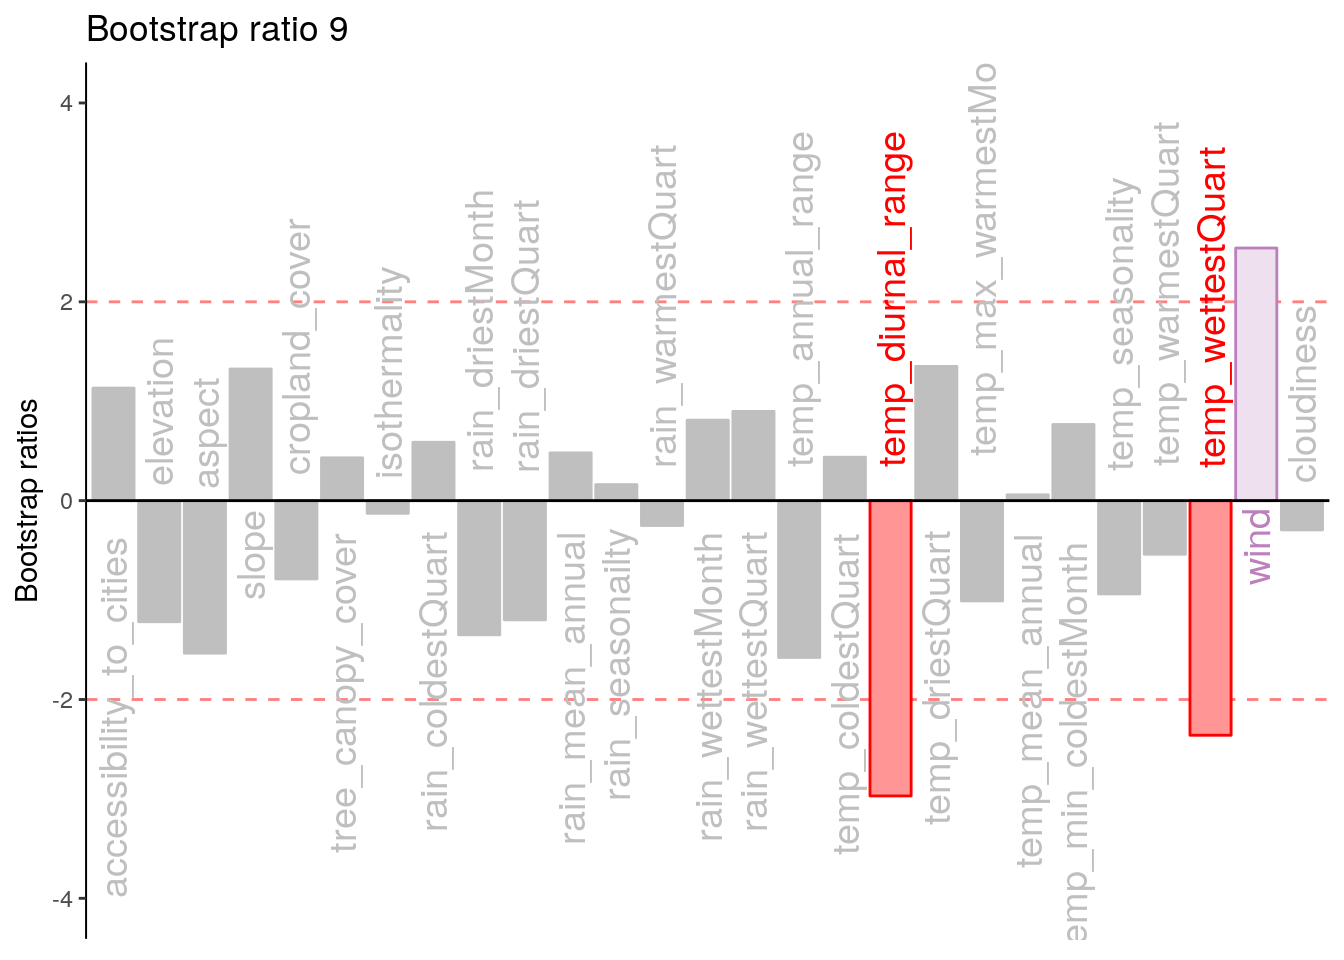
\includegraphics{Group1_Ritesh_Malaiya_PCA_Inference_World_env_vars_files/figure-latex/unnamed-chunk-14-4.pdf}

\hypertarget{bootstrap-test}{%
\paragraph{Bootstrap Test}\label{bootstrap-test}}

\begin{Shaded}
\begin{Highlighting}[]
\CommentTok{#country_env_pca_br <- PTCA4CATA::Boot4Mean(country_env_pca$ExPosition.Data$fi, design = country_env_df$Happiness_Rank, niter=100, suppressProgressBar = FALSE)}
\NormalTok{country_env_pca_bs <-}\StringTok{ }\NormalTok{data4PCCAR}\OperatorTok{::}\KeywordTok{boot.eigen}\NormalTok{(}\DataTypeTok{X =}\NormalTok{ country_env_df_for_pca, }\DataTypeTok{nIter =} \DecValTok{10000}\NormalTok{)}

\ControlFlowTok{for}\NormalTok{ (i }\ControlFlowTok{in} \KeywordTok{c}\NormalTok{(}\DecValTok{1}\NormalTok{, }\DecValTok{2}\NormalTok{, }\DecValTok{7}\NormalTok{, }\DecValTok{9}\NormalTok{)) \{}
\NormalTok{  zeDim =}\StringTok{ }\NormalTok{i}
  \KeywordTok{prettyHist}\NormalTok{(country_env_pca_bs}\OperatorTok{$}\NormalTok{boot.eigs[,zeDim], }
                    \DataTypeTok{observed =}\NormalTok{ country_env_pca_bs}\OperatorTok{$}\NormalTok{fixed.eigs[zeDim], }
                    \DataTypeTok{xlim =} \KeywordTok{c}\NormalTok{(}\DecValTok{0}\NormalTok{, }\FloatTok{4.5}\NormalTok{), }\CommentTok{# needs to set by hand}
                    \DataTypeTok{breaks =} \DecValTok{20}\NormalTok{,}
                    \DataTypeTok{border =} \StringTok{"white"}\NormalTok{, }
                    \DataTypeTok{main =} \KeywordTok{paste0}\NormalTok{(}\StringTok{"Bootstrapped distribution for Eigenvalue "}\NormalTok{,zeDim),}
                    \DataTypeTok{xlab =} \KeywordTok{paste0}\NormalTok{(}\StringTok{"Eigenvalue "}\NormalTok{,zeDim), }
                    \DataTypeTok{ylab =} \StringTok{""}\NormalTok{, }
                    \DataTypeTok{counts =} \OtherTok{FALSE}\NormalTok{, }
                    \DataTypeTok{cutoffs =} \KeywordTok{c}\NormalTok{(}\FloatTok{0.025}\NormalTok{, }\FloatTok{0.975}\NormalTok{))}
\NormalTok{\}}
\end{Highlighting}
\end{Shaded}

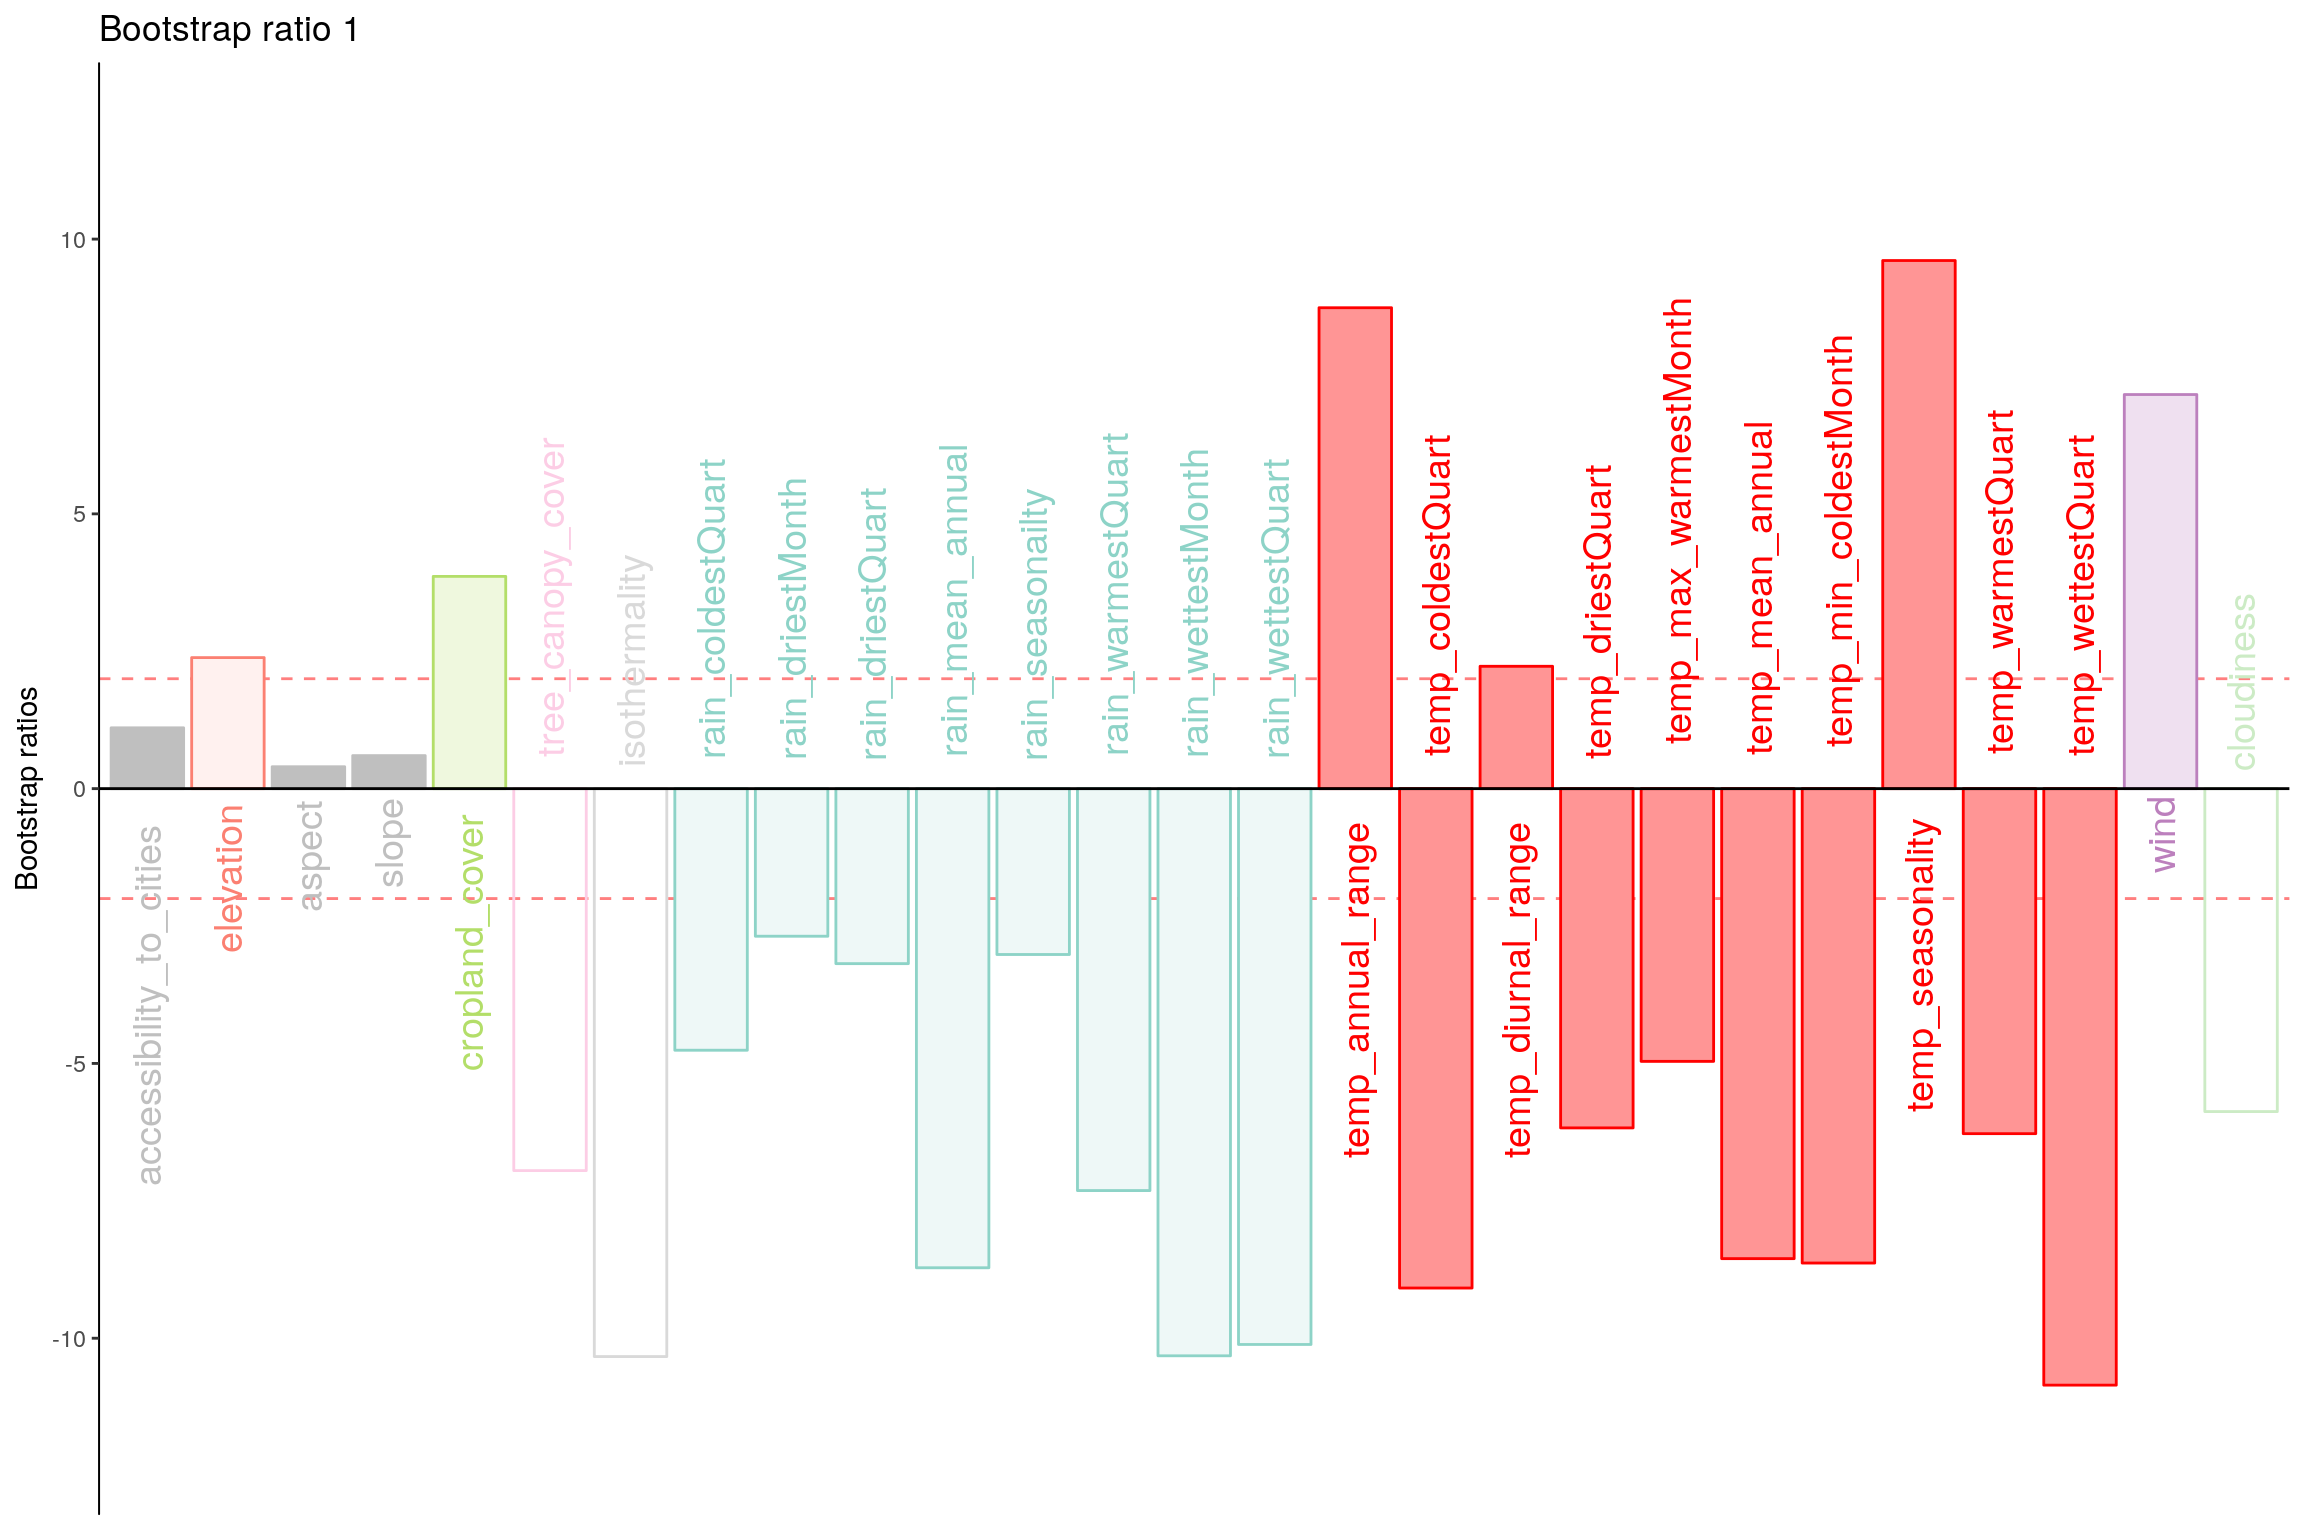
\includegraphics{Group1_Ritesh_Malaiya_PCA_Inference_World_env_vars_files/figure-latex/unnamed-chunk-15-1.pdf}
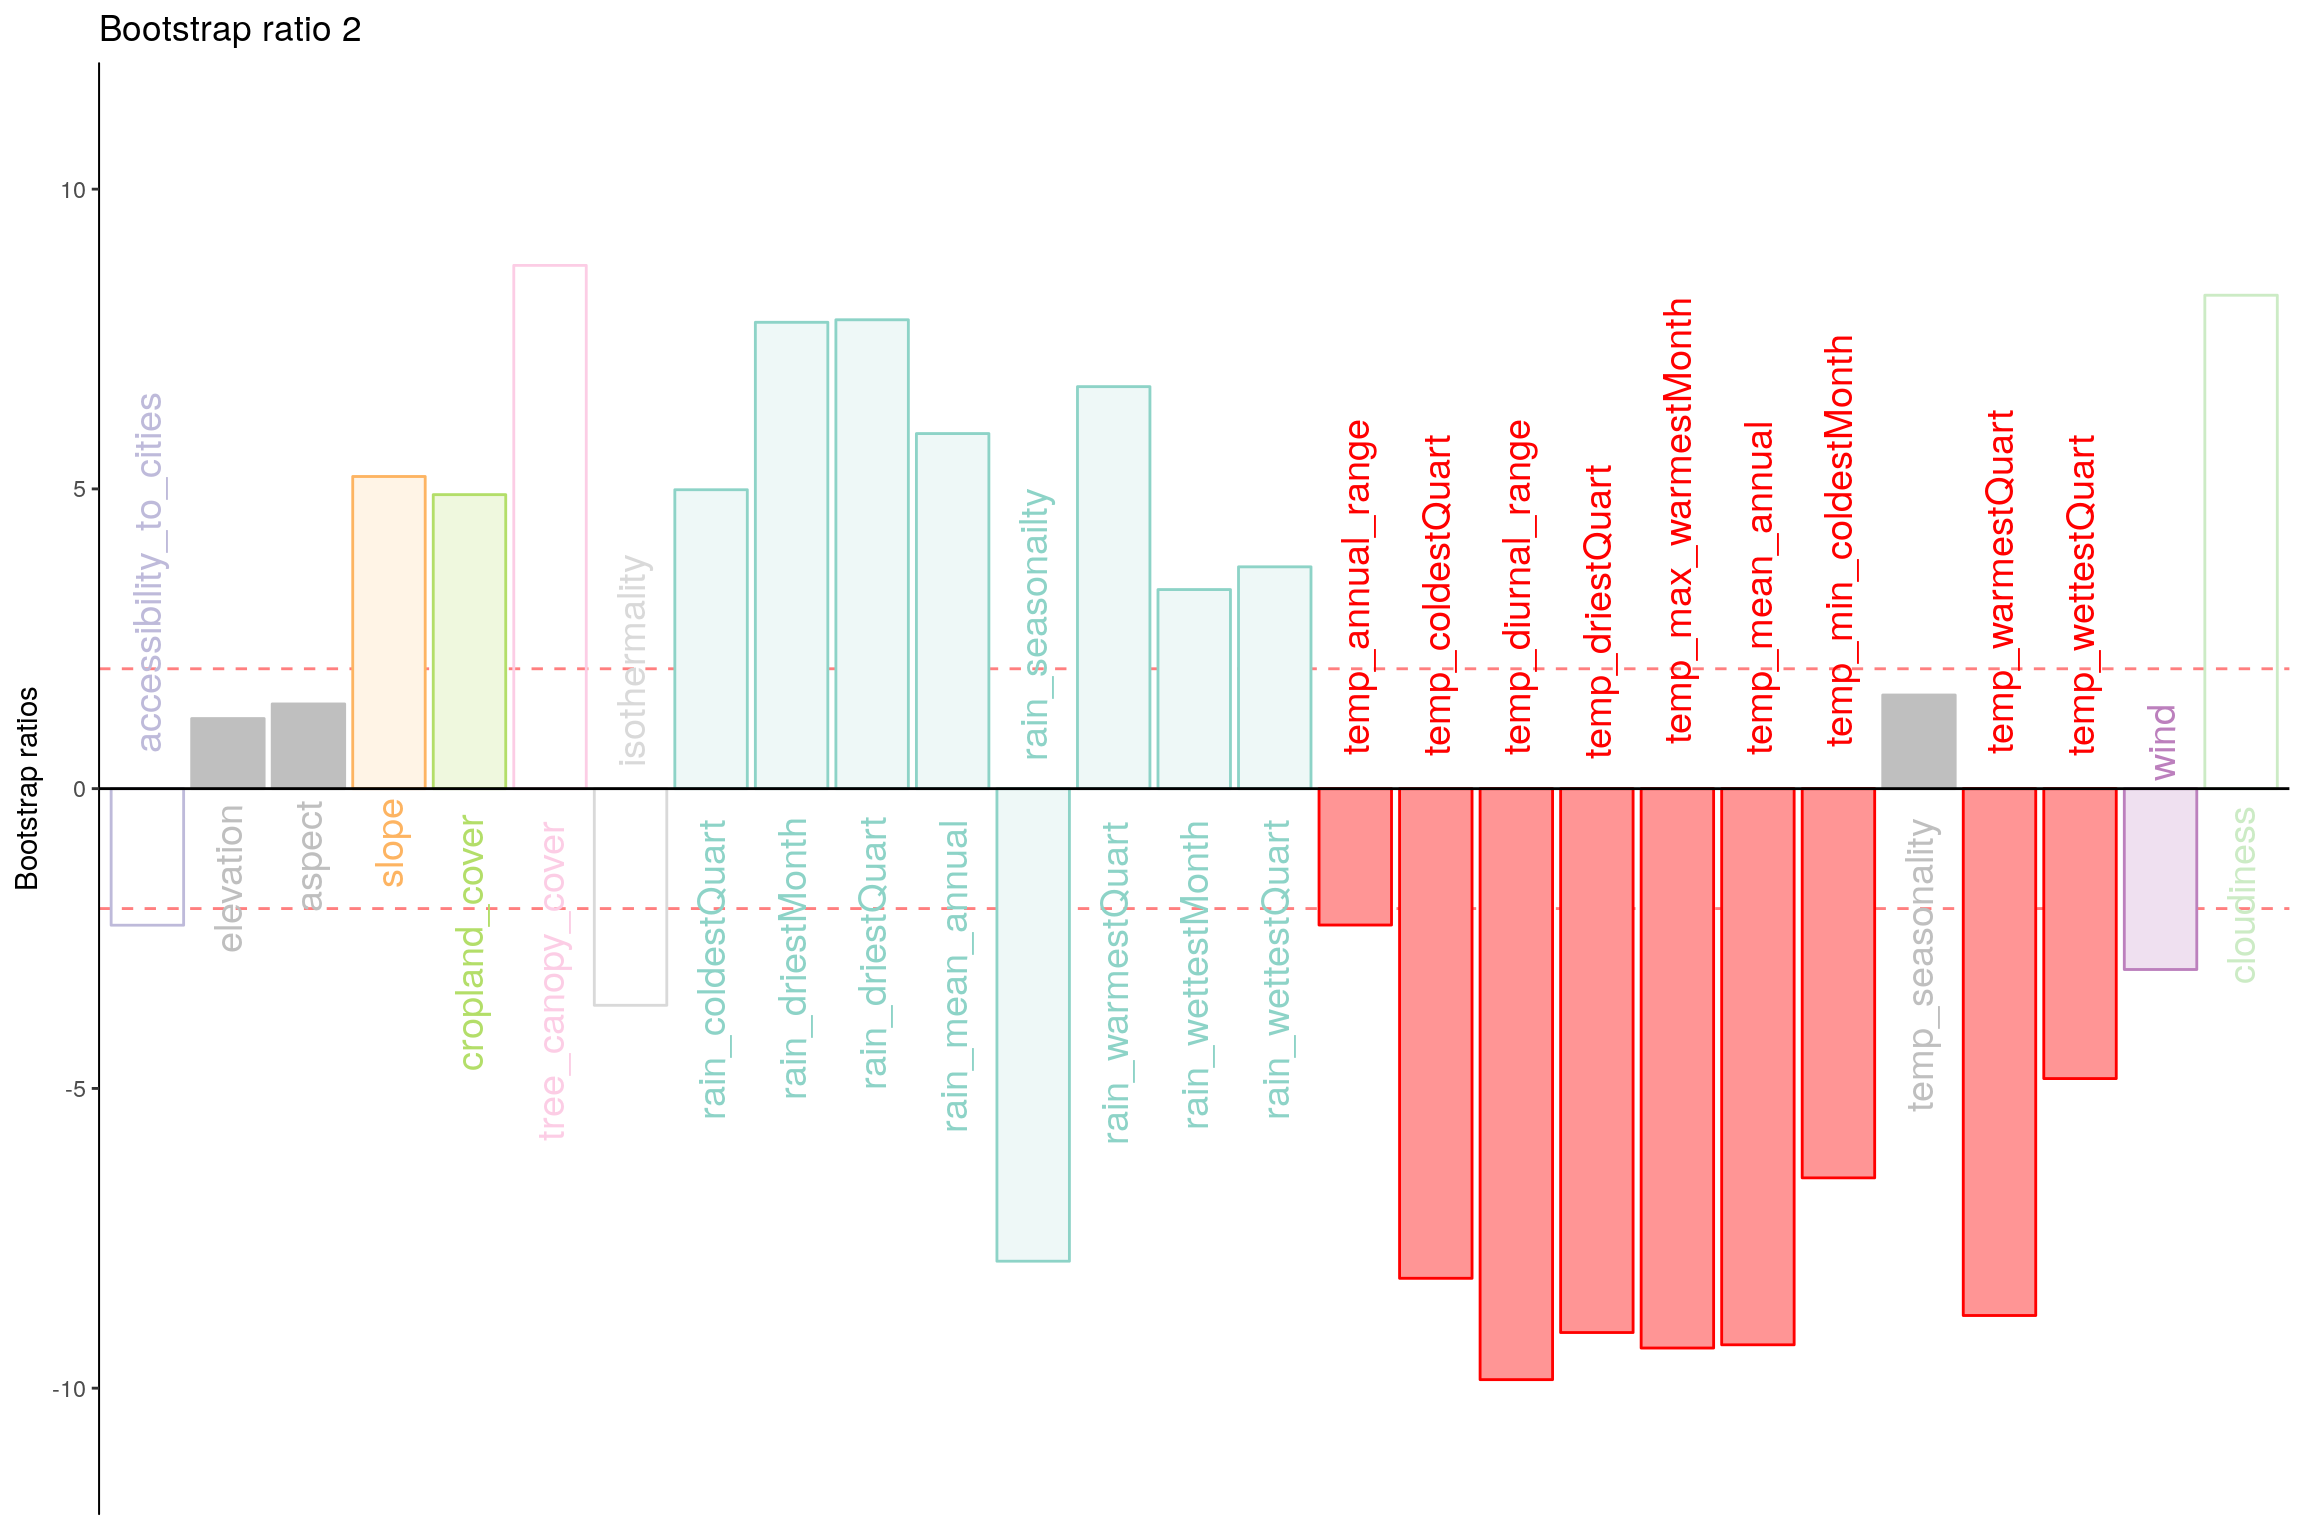
\includegraphics{Group1_Ritesh_Malaiya_PCA_Inference_World_env_vars_files/figure-latex/unnamed-chunk-15-2.pdf}
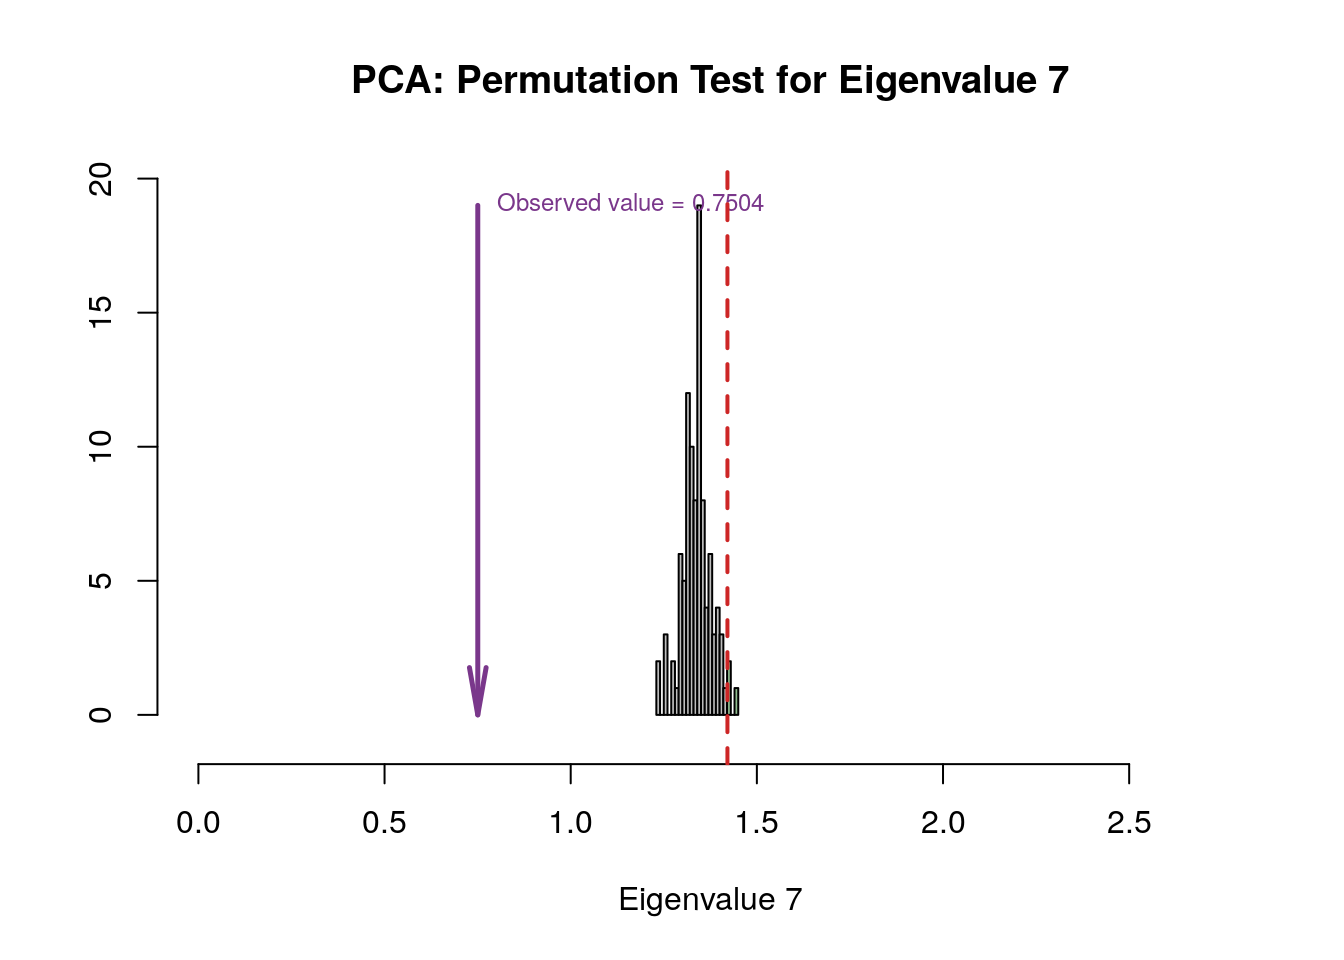
\includegraphics{Group1_Ritesh_Malaiya_PCA_Inference_World_env_vars_files/figure-latex/unnamed-chunk-15-3.pdf}
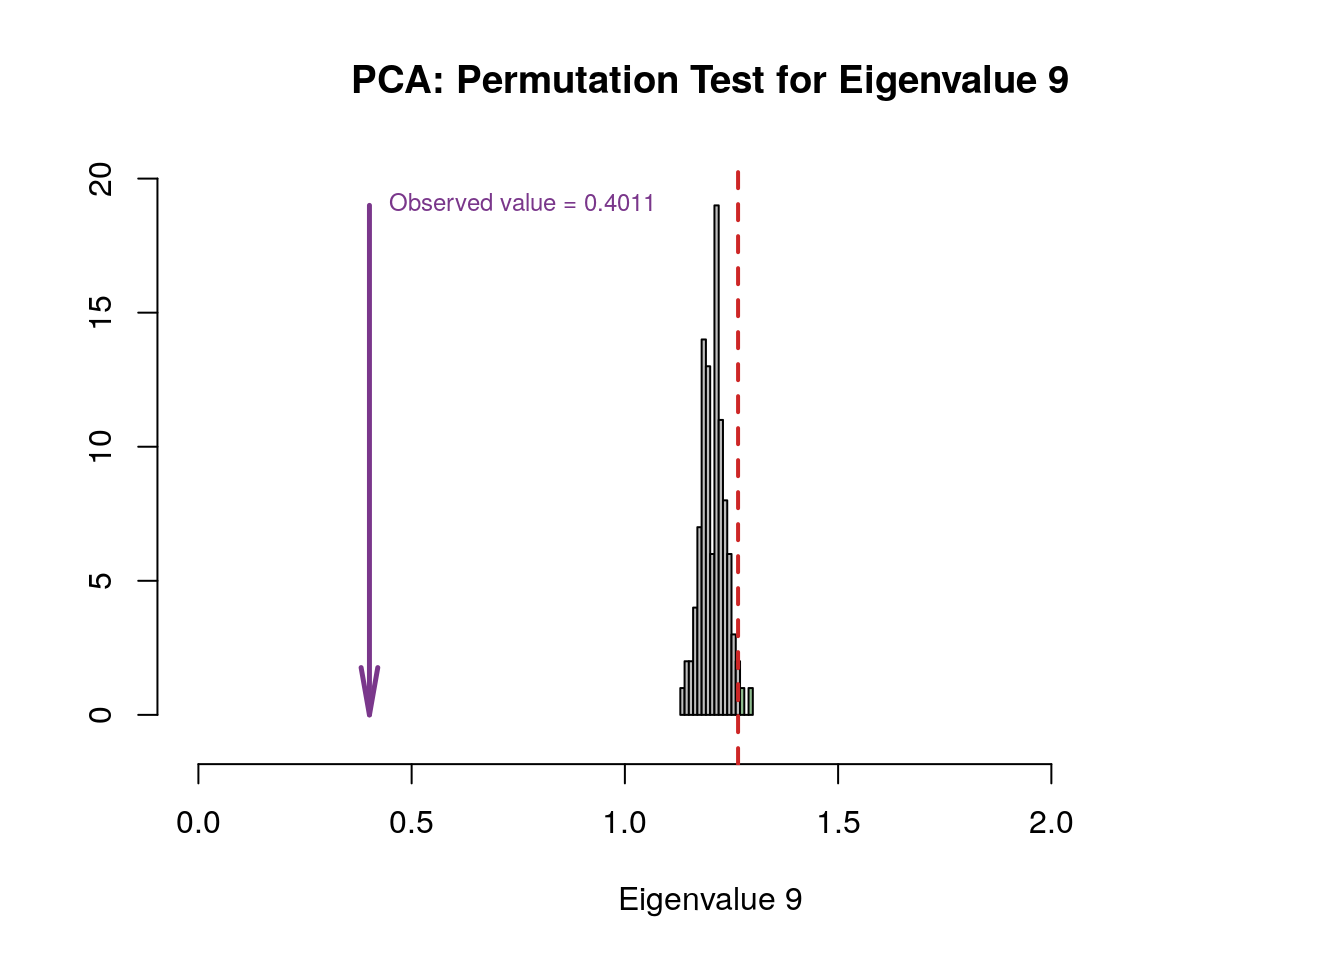
\includegraphics{Group1_Ritesh_Malaiya_PCA_Inference_World_env_vars_files/figure-latex/unnamed-chunk-15-4.pdf}

\hypertarget{bootstrap-ratios}{%
\paragraph{Bootstrap Ratios}\label{bootstrap-ratios}}

\begin{Shaded}
\begin{Highlighting}[]
\NormalTok{BR <-}\StringTok{ }\NormalTok{country_env_pca_inf}\OperatorTok{$}\NormalTok{Inference.Data}\OperatorTok{$}\NormalTok{fj.boots}\OperatorTok{$}\NormalTok{tests}\OperatorTok{$}\NormalTok{boot.ratios}

\ControlFlowTok{for}\NormalTok{ (i }\ControlFlowTok{in} \KeywordTok{c}\NormalTok{(}\DecValTok{1}\NormalTok{, }\DecValTok{2}\NormalTok{, }\DecValTok{7}\NormalTok{, }\DecValTok{9}\NormalTok{)) \{}
\NormalTok{  laDim =}\StringTok{ }\NormalTok{i}
\NormalTok{  ba001.BR1 <-}\StringTok{ }\KeywordTok{PrettyBarPlot2}\NormalTok{(BR[,laDim],}
                              \DataTypeTok{threshold =} \DecValTok{2}\NormalTok{,}
                              \DataTypeTok{font.size =} \DecValTok{5}\NormalTok{,}
                              \DataTypeTok{color4bar =}\NormalTok{ gplots}\OperatorTok{::}\KeywordTok{col2hex}\NormalTok{(col4J), }\CommentTok{# we need hex code}
                              \DataTypeTok{main =} \KeywordTok{paste0}\NormalTok{(}
                                \StringTok{'PCA on the Iris Set: Bootstrap ratio '}\NormalTok{,laDim),}
                              \DataTypeTok{ylab =} \StringTok{'Bootstrap ratios'}
                              \CommentTok{#ylim = c(1.2*min(BR[,laDim]), 1.2*max(BR[,laDim]))}
\NormalTok{  )}
  \KeywordTok{print}\NormalTok{(ba001.BR1)}
\NormalTok{\}}
\end{Highlighting}
\end{Shaded}

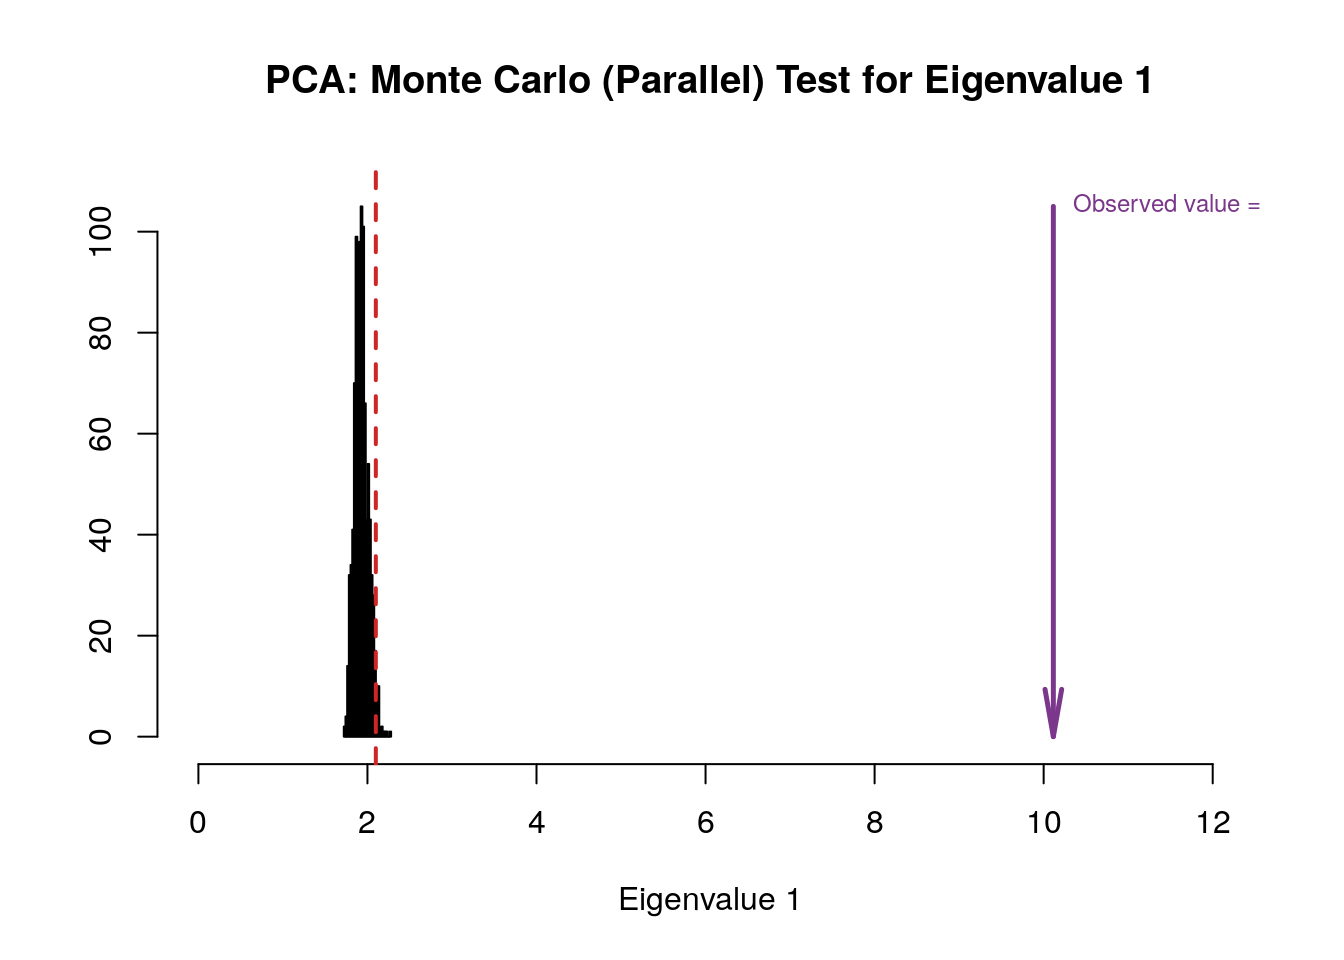
\includegraphics{Group1_Ritesh_Malaiya_PCA_Inference_World_env_vars_files/figure-latex/unnamed-chunk-16-1.pdf}
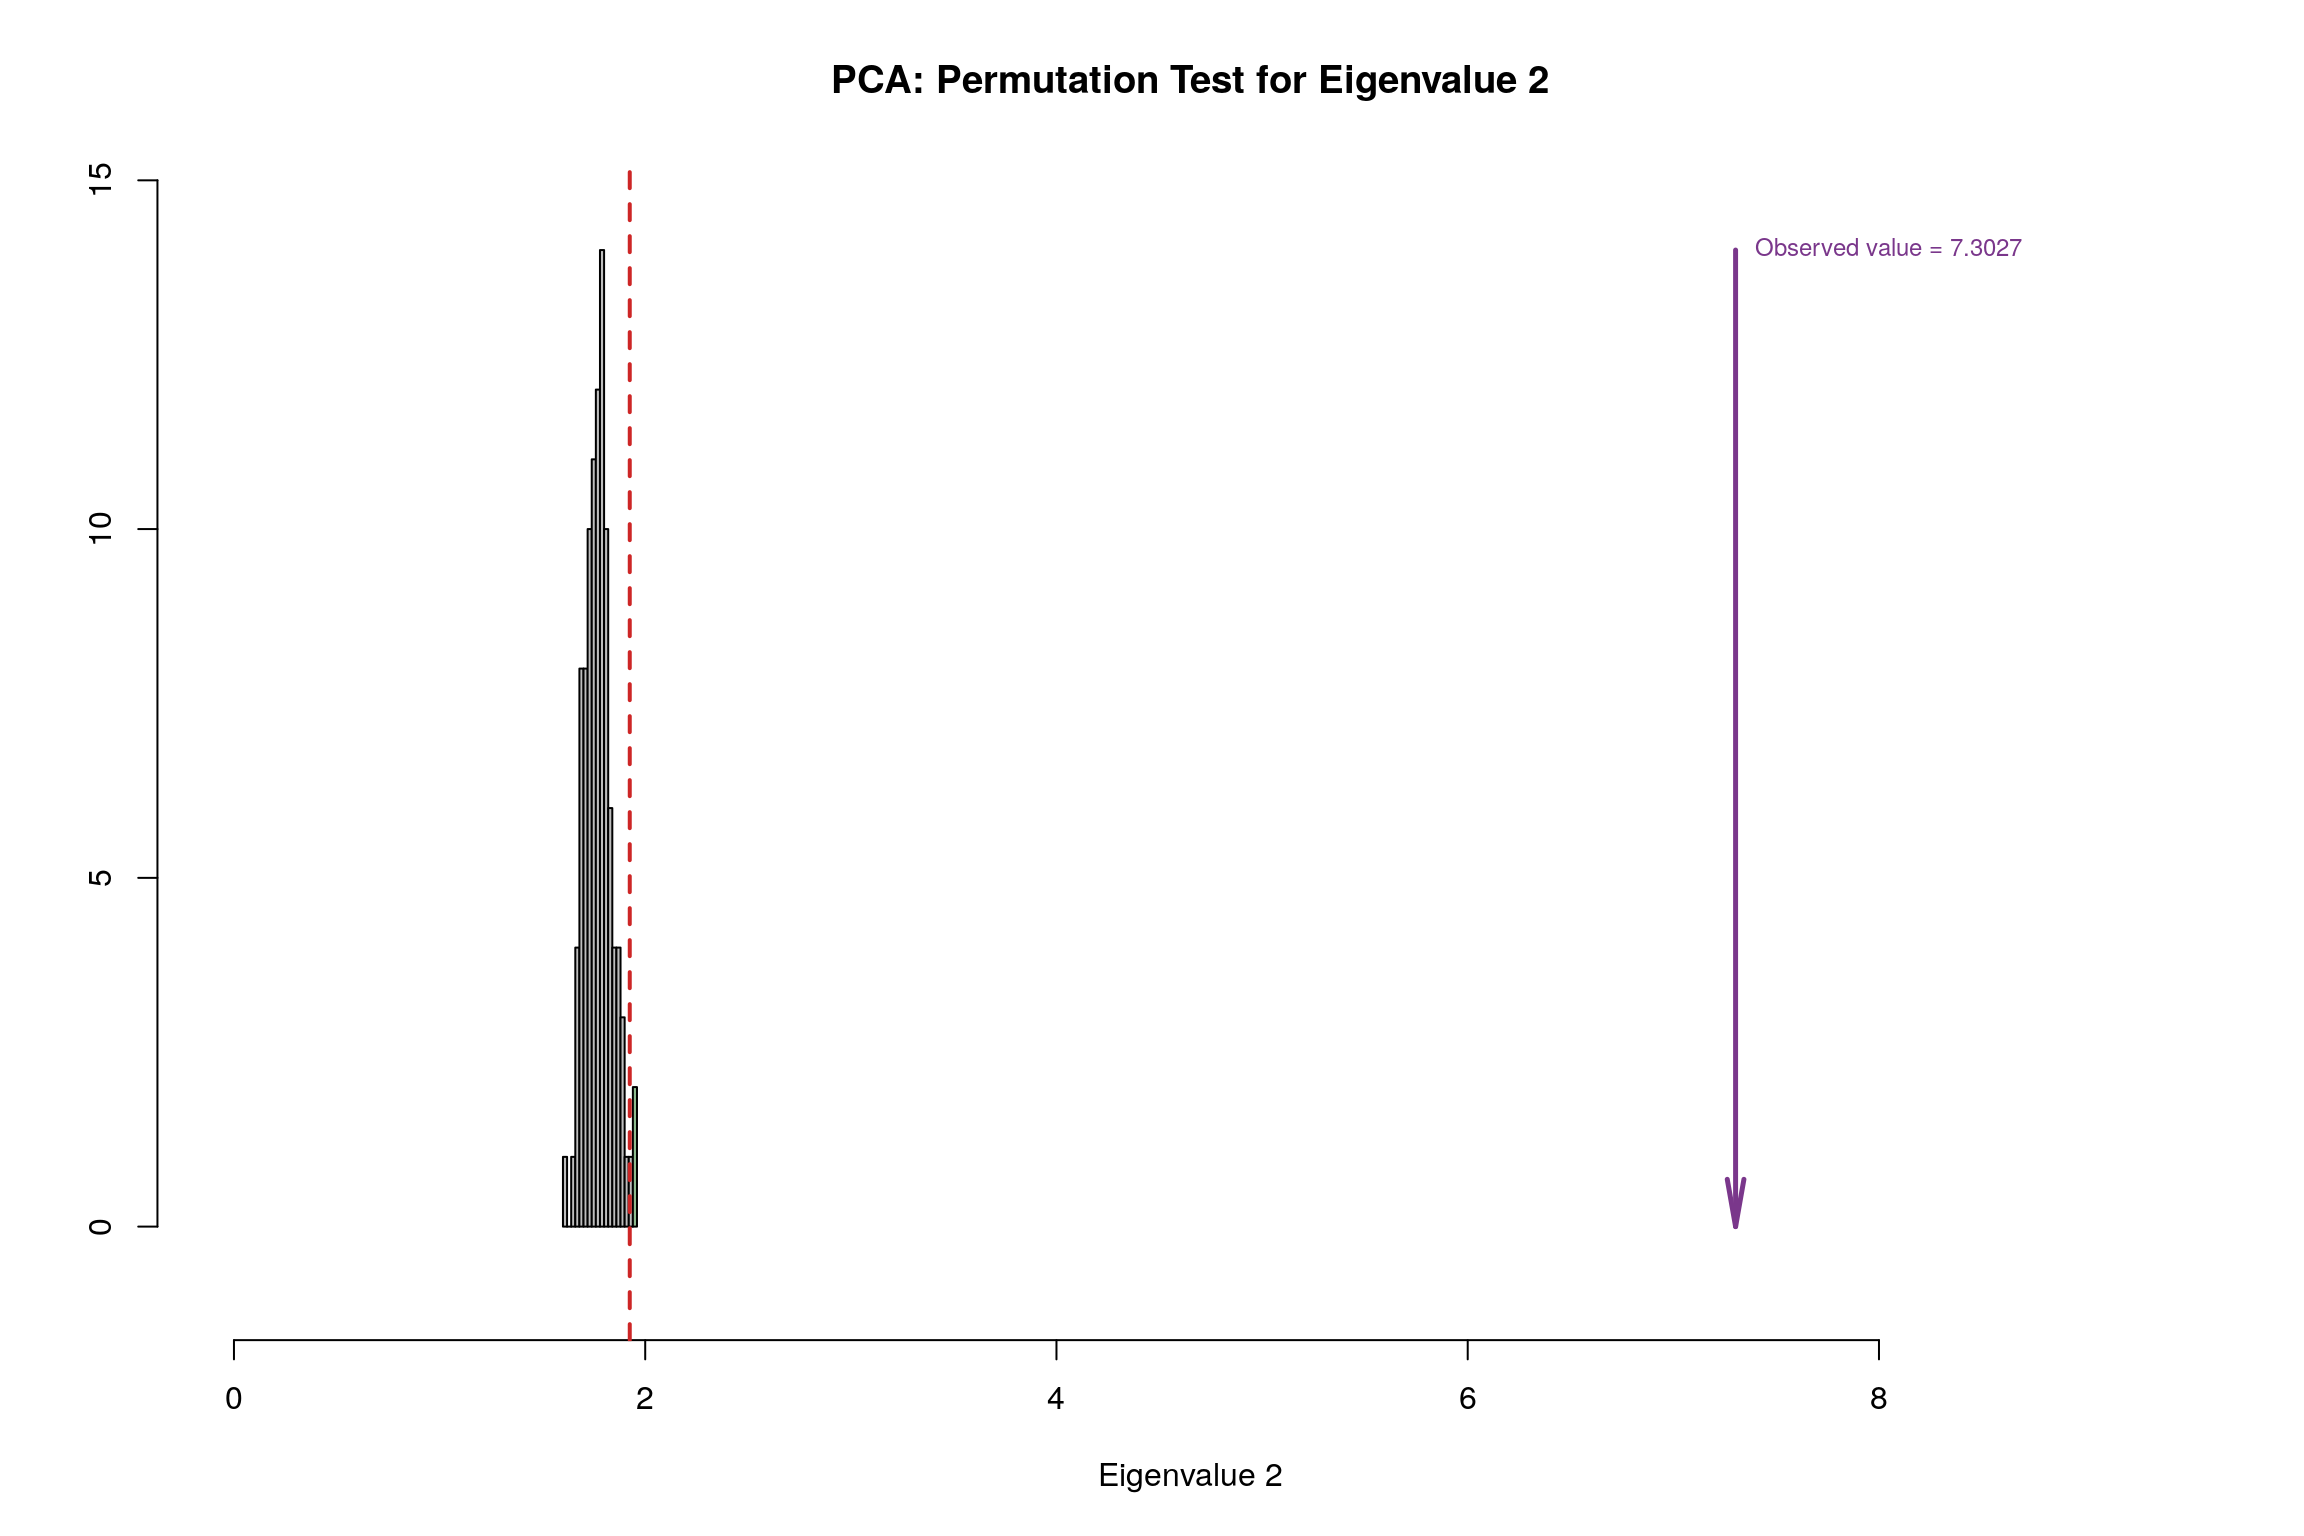
\includegraphics{Group1_Ritesh_Malaiya_PCA_Inference_World_env_vars_files/figure-latex/unnamed-chunk-16-2.pdf}
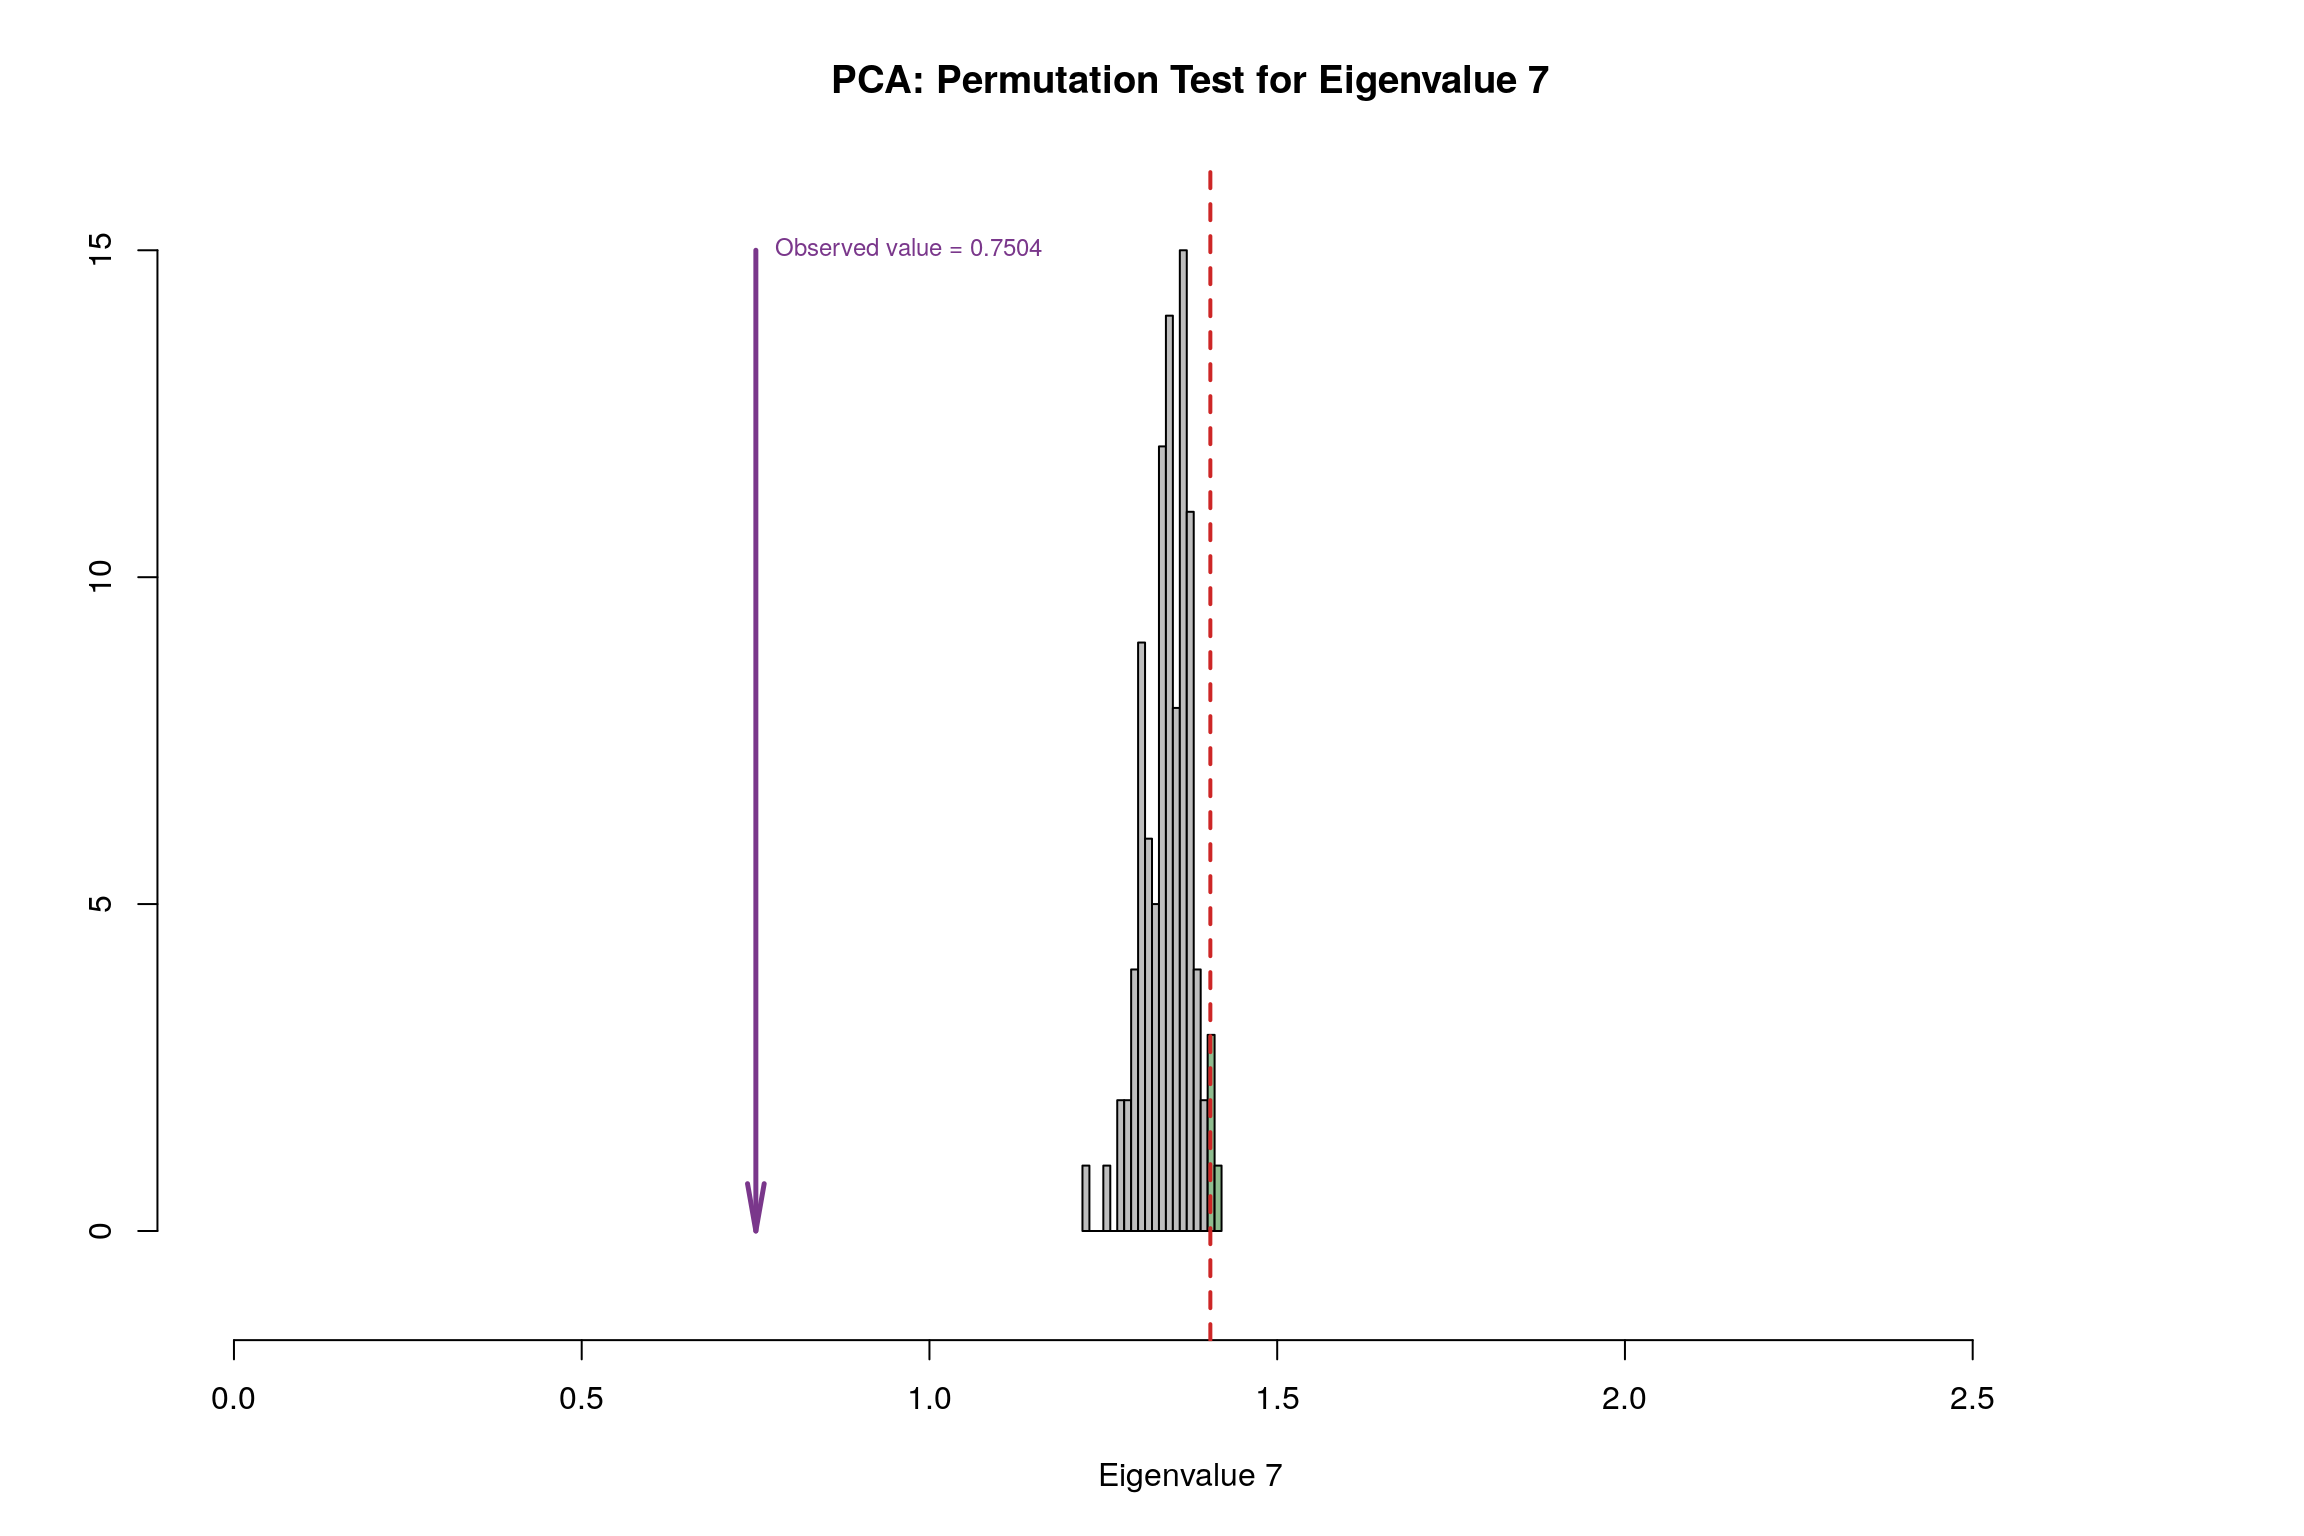
\includegraphics{Group1_Ritesh_Malaiya_PCA_Inference_World_env_vars_files/figure-latex/unnamed-chunk-16-3.pdf}
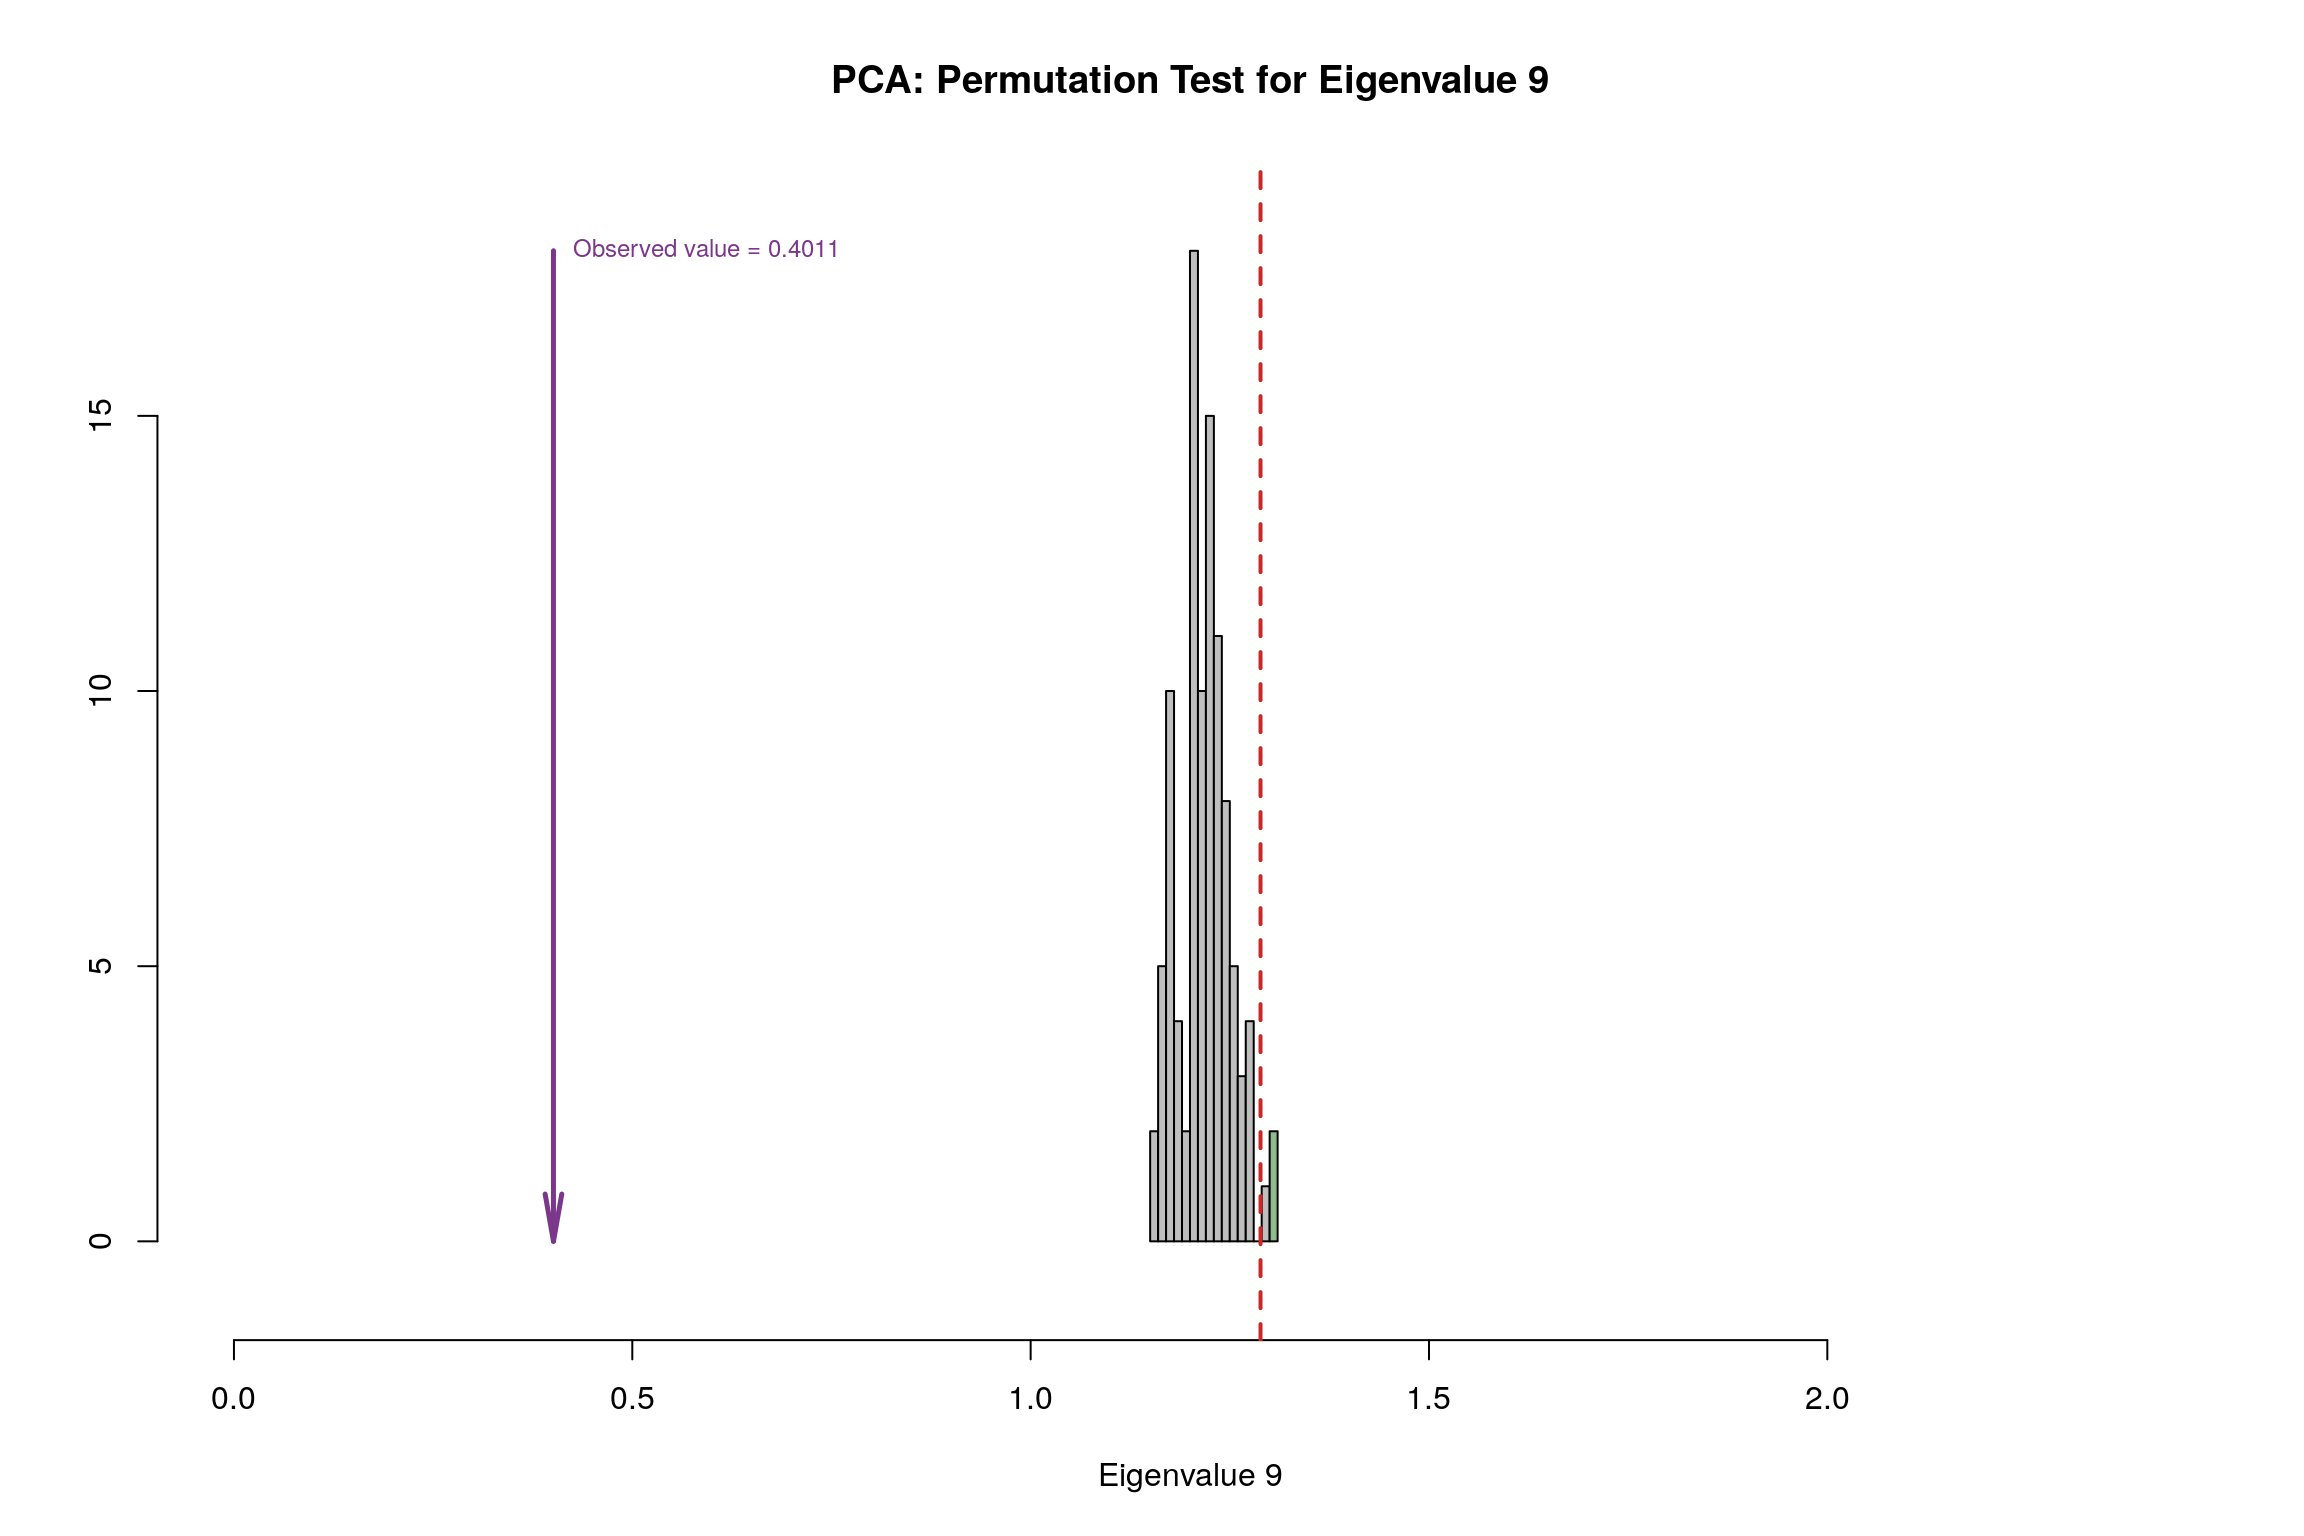
\includegraphics{Group1_Ritesh_Malaiya_PCA_Inference_World_env_vars_files/figure-latex/unnamed-chunk-16-4.pdf}

\hypertarget{confidence-interval-plot}{%
\paragraph{Confidence Interval Plot}\label{confidence-interval-plot}}

\begin{Shaded}
\begin{Highlighting}[]
\NormalTok{loop <-}\StringTok{ }\KeywordTok{matrix}\NormalTok{(}\DataTypeTok{data =} \KeywordTok{c}\NormalTok{(}\DecValTok{1}\NormalTok{,}\DecValTok{2}\NormalTok{, }\DecValTok{7}\NormalTok{,}\DecValTok{9}\NormalTok{), }\DataTypeTok{nrow =} \DecValTok{2}\NormalTok{, }\DataTypeTok{ncol =} \DecValTok{2}\NormalTok{, }\DataTypeTok{byrow =} \OtherTok{TRUE}\NormalTok{)}

\NormalTok{BootCube.Gr <-}\StringTok{ }\NormalTok{PTCA4CATA}\OperatorTok{::}\KeywordTok{Boot4Mean}\NormalTok{(country_env_pca}\OperatorTok{$}\NormalTok{ExPosition.Data}\OperatorTok{$}\NormalTok{fi, }
                                    \DataTypeTok{design =}\NormalTok{ country_env_df}\OperatorTok{$}\NormalTok{Happiness_Rank,}
                                    \DataTypeTok{niter =} \DecValTok{100}\NormalTok{,}
                                    \DataTypeTok{suppressProgressBar =} \OtherTok{TRUE}\NormalTok{)}

\ControlFlowTok{for}\NormalTok{ (i }\ControlFlowTok{in} \DecValTok{1}\OperatorTok{:}\DecValTok{2}\NormalTok{)\{}
\NormalTok{  axis1 =}\StringTok{ }\NormalTok{loop[i,}\DecValTok{1}\NormalTok{]}
\NormalTok{  axis2 =}\StringTok{ }\NormalTok{loop[i,}\DecValTok{2}\NormalTok{]}

\NormalTok{  country_factor_map <-}\StringTok{ }\NormalTok{PTCA4CATA}\OperatorTok{::}\KeywordTok{createFactorMap}\NormalTok{(country_env_pca}\OperatorTok{$}\NormalTok{ExPosition.Data}\OperatorTok{$}\NormalTok{fi, }\DataTypeTok{title=}\StringTok{''}\NormalTok{, }
                                                 \DataTypeTok{col.points =}\NormalTok{ country_env_pca}\OperatorTok{$}\NormalTok{Plotting.Data}\OperatorTok{$}\NormalTok{fi.col,}
                                                 \DataTypeTok{col.labels =}\NormalTok{ country_env_pca}\OperatorTok{$}\NormalTok{Plotting.Data}\OperatorTok{$}\NormalTok{fi.col,}
                                                 \DataTypeTok{axis1 =}\NormalTok{ axis1,}
                                                 \DataTypeTok{axis2 =}\NormalTok{ axis2,}
                                                 \DataTypeTok{display.labels =} \OtherTok{FALSE}\NormalTok{)}

\NormalTok{country_factor_map_mean <-}\StringTok{ }\NormalTok{PTCA4CATA}\OperatorTok{::}\KeywordTok{createFactorMap}\NormalTok{(country_env_pca_mean,}
                                                 \DataTypeTok{col.points =} \KeywordTok{unique}\NormalTok{(country_env_pca}\OperatorTok{$}\NormalTok{Plotting.Data}\OperatorTok{$}\NormalTok{fi.col),}
                                                 \DataTypeTok{col.labels =} \KeywordTok{unique}\NormalTok{(country_env_pca}\OperatorTok{$}\NormalTok{Plotting.Data}\OperatorTok{$}\NormalTok{fi.col),}
                                                 \DataTypeTok{axis1 =}\NormalTok{ axis1,}
                                                 \DataTypeTok{axis2 =}\NormalTok{ axis2,}
                                                 \DataTypeTok{display.labels =} \OtherTok{TRUE}\NormalTok{,}
                                                 \DataTypeTok{cex =} \DecValTok{8}\NormalTok{,}\DataTypeTok{alpha.points =} \FloatTok{0.8}\NormalTok{)}

\NormalTok{country_label4Map <-}\StringTok{ }\NormalTok{PTCA4CATA}\OperatorTok{::}\KeywordTok{createxyLabels.gen}\NormalTok{(axis1,axis2,}\DataTypeTok{lambda =}\NormalTok{ country_env_pca}\OperatorTok{$}\NormalTok{ExPosition.Data}\OperatorTok{$}\NormalTok{eigs, }\DataTypeTok{tau =}\NormalTok{ country_env_pca}\OperatorTok{$}\NormalTok{ExPosition.Data}\OperatorTok{$}\NormalTok{t) }



\NormalTok{country_map =}\StringTok{ }\NormalTok{country_factor_map}\OperatorTok{$}\NormalTok{zeMap }\OperatorTok{+}\StringTok{ }\NormalTok{country_label4Map }\OperatorTok{+}\StringTok{ }\NormalTok{country_factor_map_mean}\OperatorTok{$}\NormalTok{zeMap_dots }\OperatorTok{+}\StringTok{ }\NormalTok{country_factor_map_mean}\OperatorTok{$}\NormalTok{zeMap_text}


\NormalTok{GraphElli <-}\StringTok{ }\NormalTok{PTCA4CATA}\OperatorTok{::}\KeywordTok{MakeCIEllipses}\NormalTok{(BootCube.Gr}\OperatorTok{$}\NormalTok{BootCube[,}\KeywordTok{c}\NormalTok{(axis1, axis2),],}
                                       \DataTypeTok{names.of.factors =} \KeywordTok{c}\NormalTok{(}\KeywordTok{paste}\NormalTok{(}\StringTok{"Dimension"}\NormalTok{,axis1), }\KeywordTok{paste}\NormalTok{(}\StringTok{"Dimension"}\NormalTok{,axis2)),}
                                       \DataTypeTok{col =} \KeywordTok{unique}\NormalTok{(country_env_pca}\OperatorTok{$}\NormalTok{Plotting.Data}\OperatorTok{$}\NormalTok{fi.col),}
                                       \DataTypeTok{p.level =} \FloatTok{.95}
\NormalTok{)}

\NormalTok{country_map =}\StringTok{ }\NormalTok{country_map }\OperatorTok{+}\StringTok{ }\NormalTok{GraphElli}

\KeywordTok{print}\NormalTok{(country_map)}


\NormalTok{\}}
\end{Highlighting}
\end{Shaded}

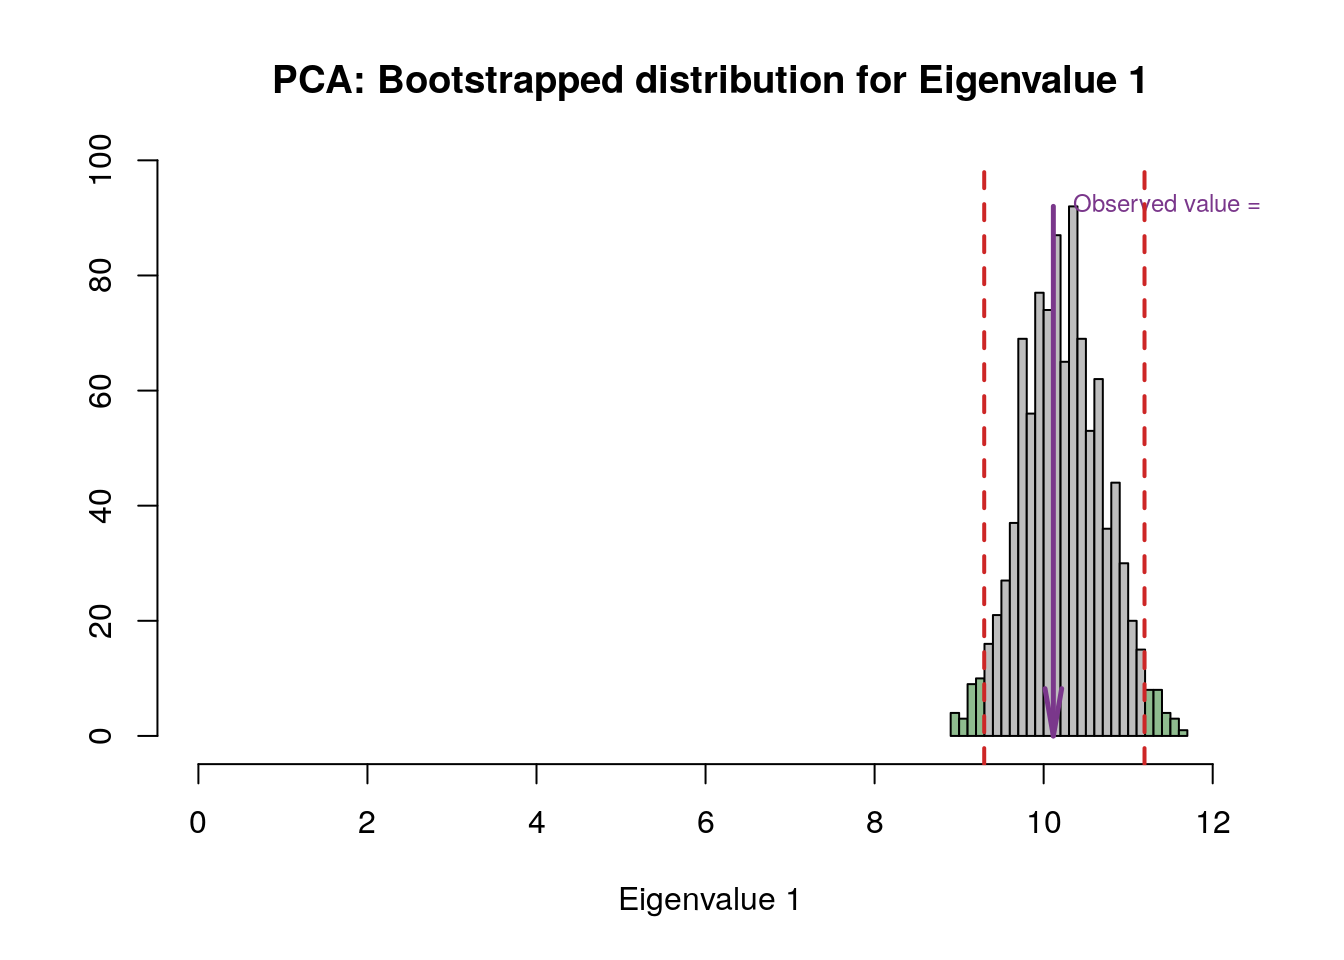
\includegraphics{Group1_Ritesh_Malaiya_PCA_Inference_World_env_vars_files/figure-latex/unnamed-chunk-17-1.pdf}
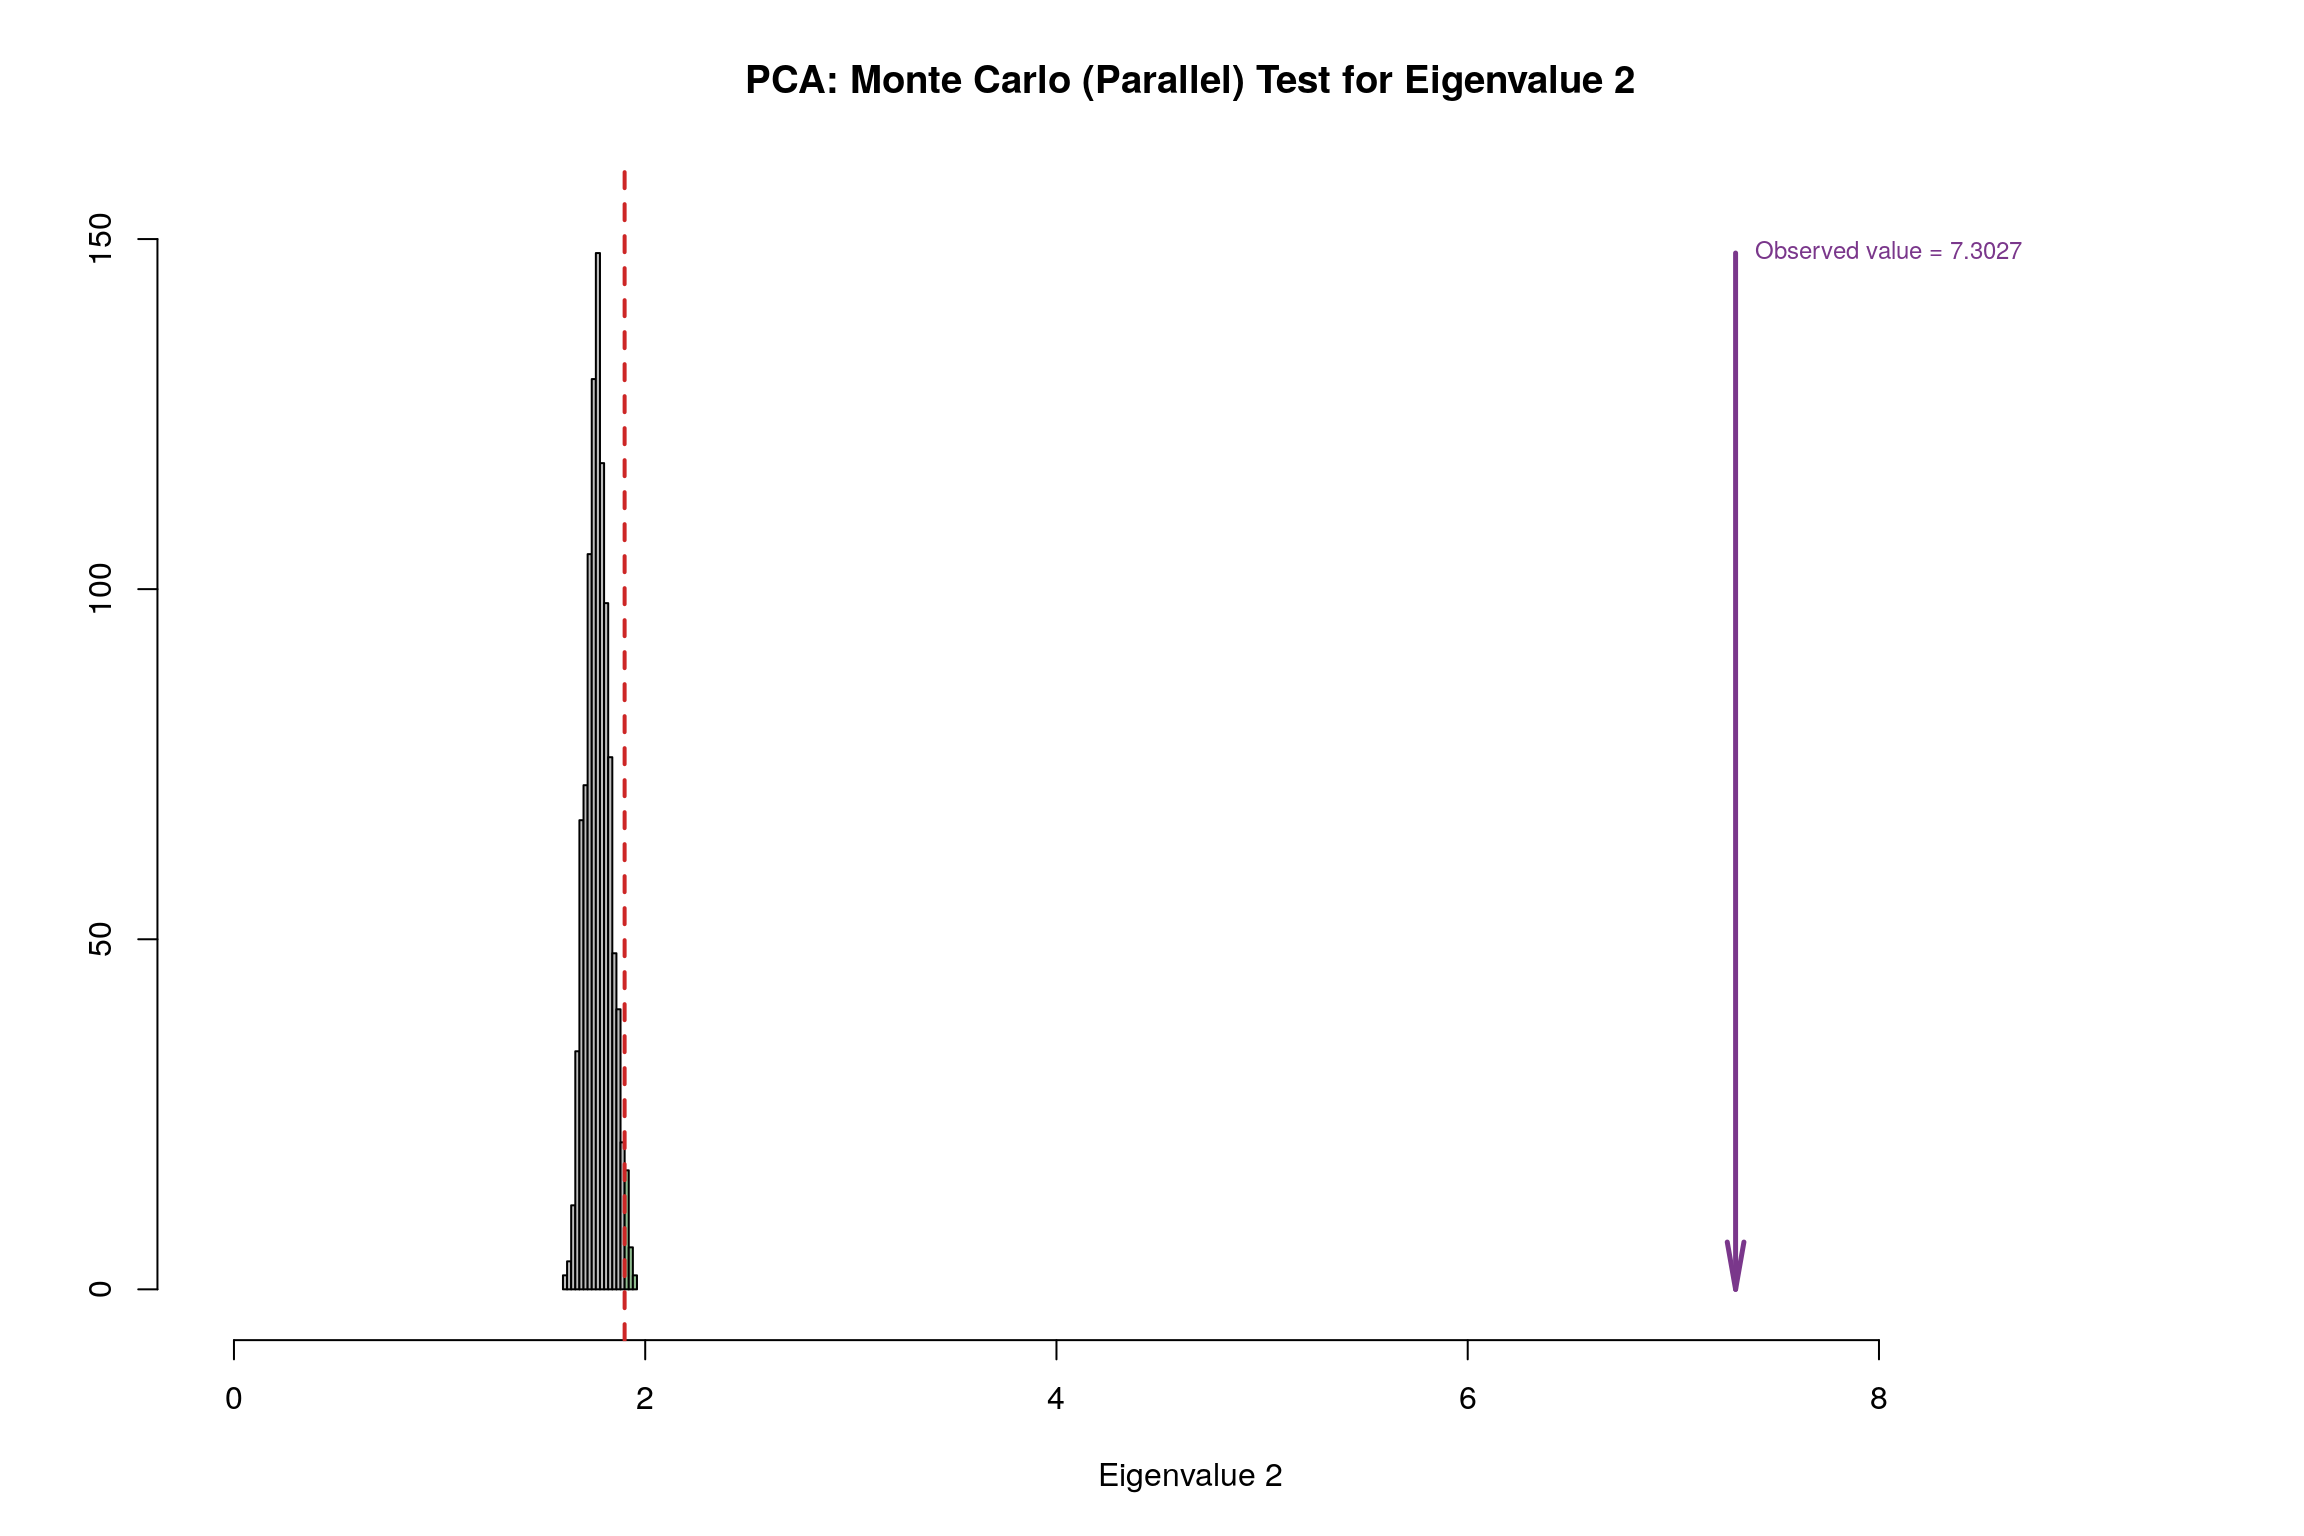
\includegraphics{Group1_Ritesh_Malaiya_PCA_Inference_World_env_vars_files/figure-latex/unnamed-chunk-17-2.pdf}

\hypertarget{tolerance-interval-plot}{%
\paragraph{Tolerance Interval Plot}\label{tolerance-interval-plot}}

\begin{Shaded}
\begin{Highlighting}[]
\NormalTok{loop <-}\StringTok{ }\KeywordTok{matrix}\NormalTok{(}\DataTypeTok{data =} \KeywordTok{c}\NormalTok{(}\DecValTok{1}\NormalTok{,}\DecValTok{2}\NormalTok{, }\DecValTok{7}\NormalTok{,}\DecValTok{9}\NormalTok{), }\DataTypeTok{nrow =} \DecValTok{2}\NormalTok{, }\DataTypeTok{ncol =} \DecValTok{2}\NormalTok{, }\DataTypeTok{byrow =} \OtherTok{TRUE}\NormalTok{)}

\ControlFlowTok{for}\NormalTok{ (i }\ControlFlowTok{in} \DecValTok{1}\OperatorTok{:}\DecValTok{2}\NormalTok{)\{}
\NormalTok{  axis1 =}\StringTok{ }\NormalTok{loop[i,}\DecValTok{1}\NormalTok{]}
\NormalTok{  axis2 =}\StringTok{ }\NormalTok{loop[i,}\DecValTok{2}\NormalTok{]}

\NormalTok{country_factor_map <-}\StringTok{ }\NormalTok{PTCA4CATA}\OperatorTok{::}\KeywordTok{createFactorMap}\NormalTok{(country_env_pca}\OperatorTok{$}\NormalTok{ExPosition.Data}\OperatorTok{$}\NormalTok{fi, }\DataTypeTok{title=}\StringTok{''}\NormalTok{, }
                                                 \DataTypeTok{col.points =}\NormalTok{ country_env_pca}\OperatorTok{$}\NormalTok{Plotting.Data}\OperatorTok{$}\NormalTok{fi.col,}
                                                 \DataTypeTok{col.labels =}\NormalTok{ country_env_pca}\OperatorTok{$}\NormalTok{Plotting.Data}\OperatorTok{$}\NormalTok{fi.col,}
                                                 \DataTypeTok{axis1 =}\NormalTok{ axis1,}
                                                 \DataTypeTok{axis2 =}\NormalTok{ axis2,}
                                                 \DataTypeTok{display.labels =} \OtherTok{FALSE}\NormalTok{)}

\NormalTok{country_factor_map_mean <-}\StringTok{ }\NormalTok{PTCA4CATA}\OperatorTok{::}\KeywordTok{createFactorMap}\NormalTok{(country_env_pca_mean,}
                                                 \DataTypeTok{col.points =} \KeywordTok{unique}\NormalTok{(country_env_pca}\OperatorTok{$}\NormalTok{Plotting.Data}\OperatorTok{$}\NormalTok{fi.col),}
                                                 \DataTypeTok{col.labels =} \KeywordTok{unique}\NormalTok{(country_env_pca}\OperatorTok{$}\NormalTok{Plotting.Data}\OperatorTok{$}\NormalTok{fi.col),}
                                                 \DataTypeTok{axis1 =}\NormalTok{ axis1,}
                                                 \DataTypeTok{axis2 =}\NormalTok{ axis2,}
                                                 \DataTypeTok{display.labels =} \OtherTok{TRUE}\NormalTok{,}
                                                 \DataTypeTok{cex =} \DecValTok{8}\NormalTok{,}\DataTypeTok{alpha.points =} \FloatTok{0.8}\NormalTok{)}

\NormalTok{country_label4Map <-}\StringTok{ }\NormalTok{PTCA4CATA}\OperatorTok{::}\KeywordTok{createxyLabels.gen}\NormalTok{(axis1,axis2,}\DataTypeTok{lambda =}\NormalTok{ country_env_pca}\OperatorTok{$}\NormalTok{ExPosition.Data}\OperatorTok{$}\NormalTok{eigs, }\DataTypeTok{tau =}\NormalTok{ country_env_pca}\OperatorTok{$}\NormalTok{ExPosition.Data}\OperatorTok{$}\NormalTok{t) }



\NormalTok{country_map =}\StringTok{ }\NormalTok{country_factor_map}\OperatorTok{$}\NormalTok{zeMap }\OperatorTok{+}\StringTok{ }\NormalTok{country_label4Map }\OperatorTok{+}\StringTok{ }\NormalTok{country_factor_map_mean}\OperatorTok{$}\NormalTok{zeMap_dots }\OperatorTok{+}\StringTok{ }\NormalTok{country_factor_map_mean}\OperatorTok{$}\NormalTok{zeMap_text}


\NormalTok{GraphTI.Hull <-}\StringTok{ }\NormalTok{PTCA4CATA}\OperatorTok{::}\KeywordTok{MakeToleranceIntervals}\NormalTok{(country_env_pca}\OperatorTok{$}\NormalTok{ExPosition.Data}\OperatorTok{$}\NormalTok{fi[,}\KeywordTok{c}\NormalTok{(axis1, axis2)],}
                                                  \DataTypeTok{design =}\NormalTok{ country_env_df}\OperatorTok{$}\NormalTok{Happiness_Rank,}
                                                  \CommentTok{# line below is needed}
                                                  \DataTypeTok{names.of.factors =}  \KeywordTok{c}\NormalTok{(}\StringTok{"Dim1"}\NormalTok{,}\StringTok{"Dim2"}\NormalTok{), }\CommentTok{# needed }
                                                  \DataTypeTok{col =} \KeywordTok{unique}\NormalTok{(country_env_pca}\OperatorTok{$}\NormalTok{Plotting.Data}\OperatorTok{$}\NormalTok{fi.col),}
                                                  \DataTypeTok{line.size =} \FloatTok{.50}\NormalTok{, }
                                                  \DataTypeTok{line.type =} \DecValTok{3}\NormalTok{,}
                                                  \DataTypeTok{alpha.ellipse =} \FloatTok{.2}\NormalTok{,}
                                                  \DataTypeTok{alpha.line    =} \FloatTok{.4}\NormalTok{,}
                                                  \DataTypeTok{p.level       =} \FloatTok{.75}\NormalTok{)}

\NormalTok{country_map =}\StringTok{ }\NormalTok{country_map }\OperatorTok{+}\StringTok{ }\NormalTok{GraphTI.Hull}

\KeywordTok{print}\NormalTok{(country_map)}


\NormalTok{\}}
\end{Highlighting}
\end{Shaded}

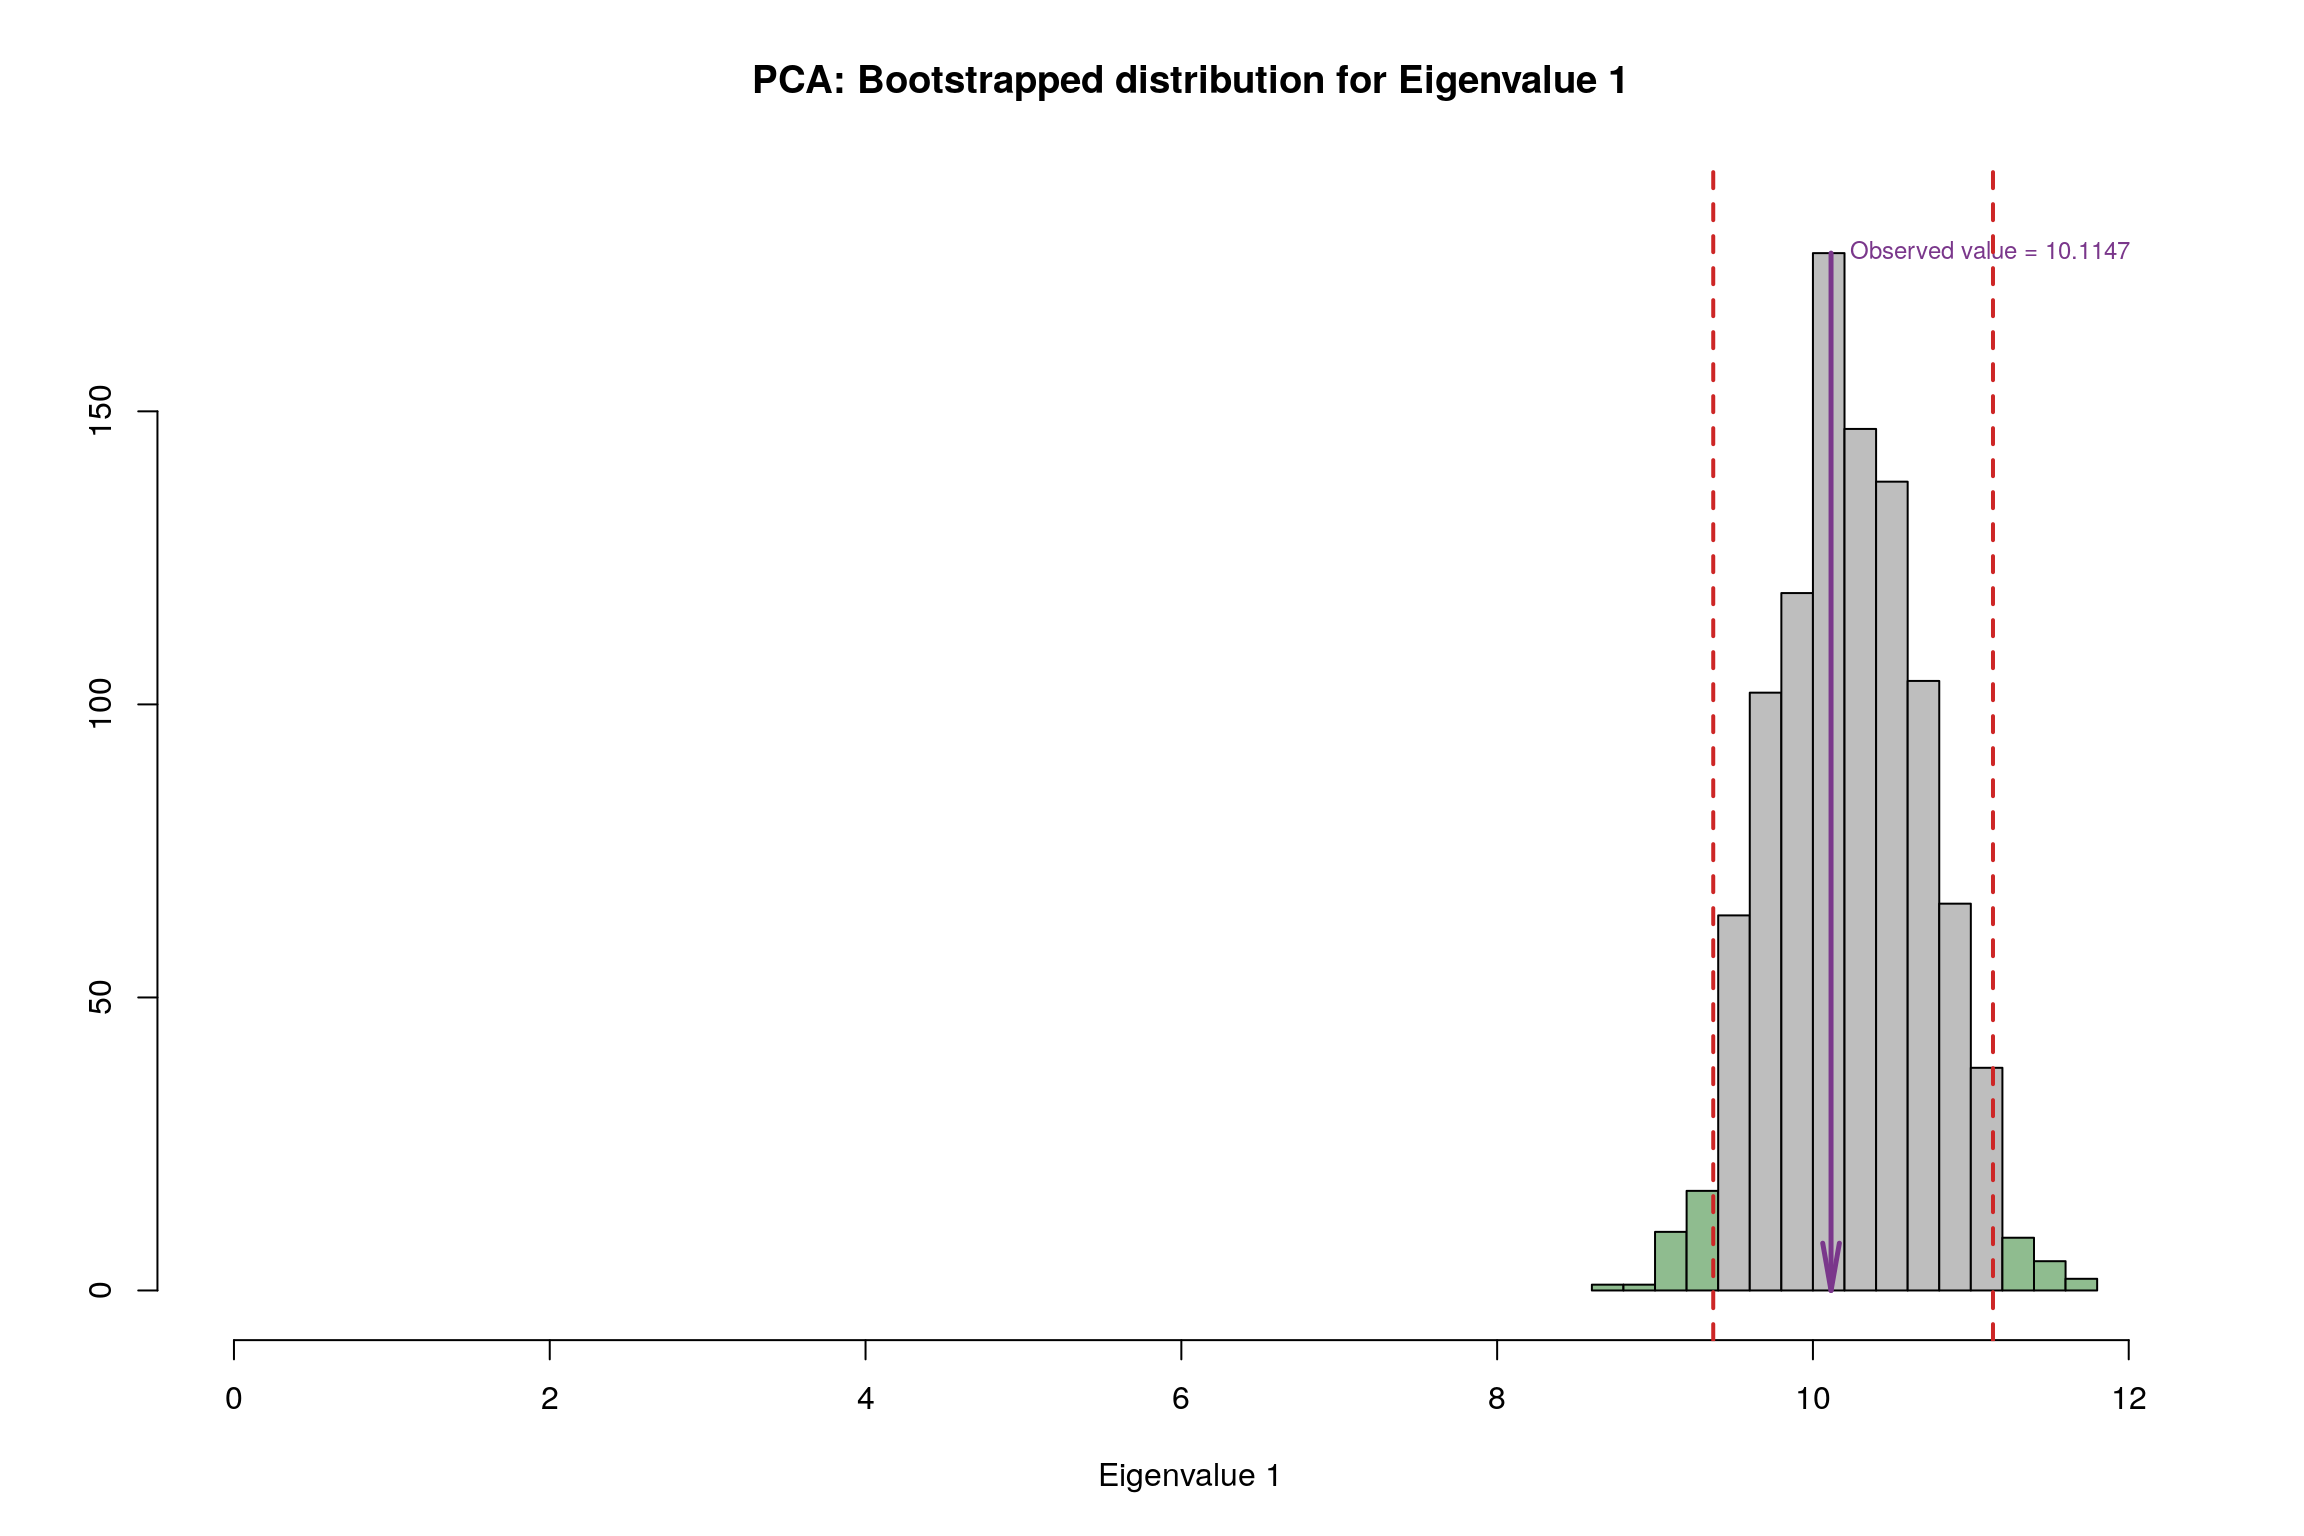
\includegraphics{Group1_Ritesh_Malaiya_PCA_Inference_World_env_vars_files/figure-latex/unnamed-chunk-18-1.pdf}
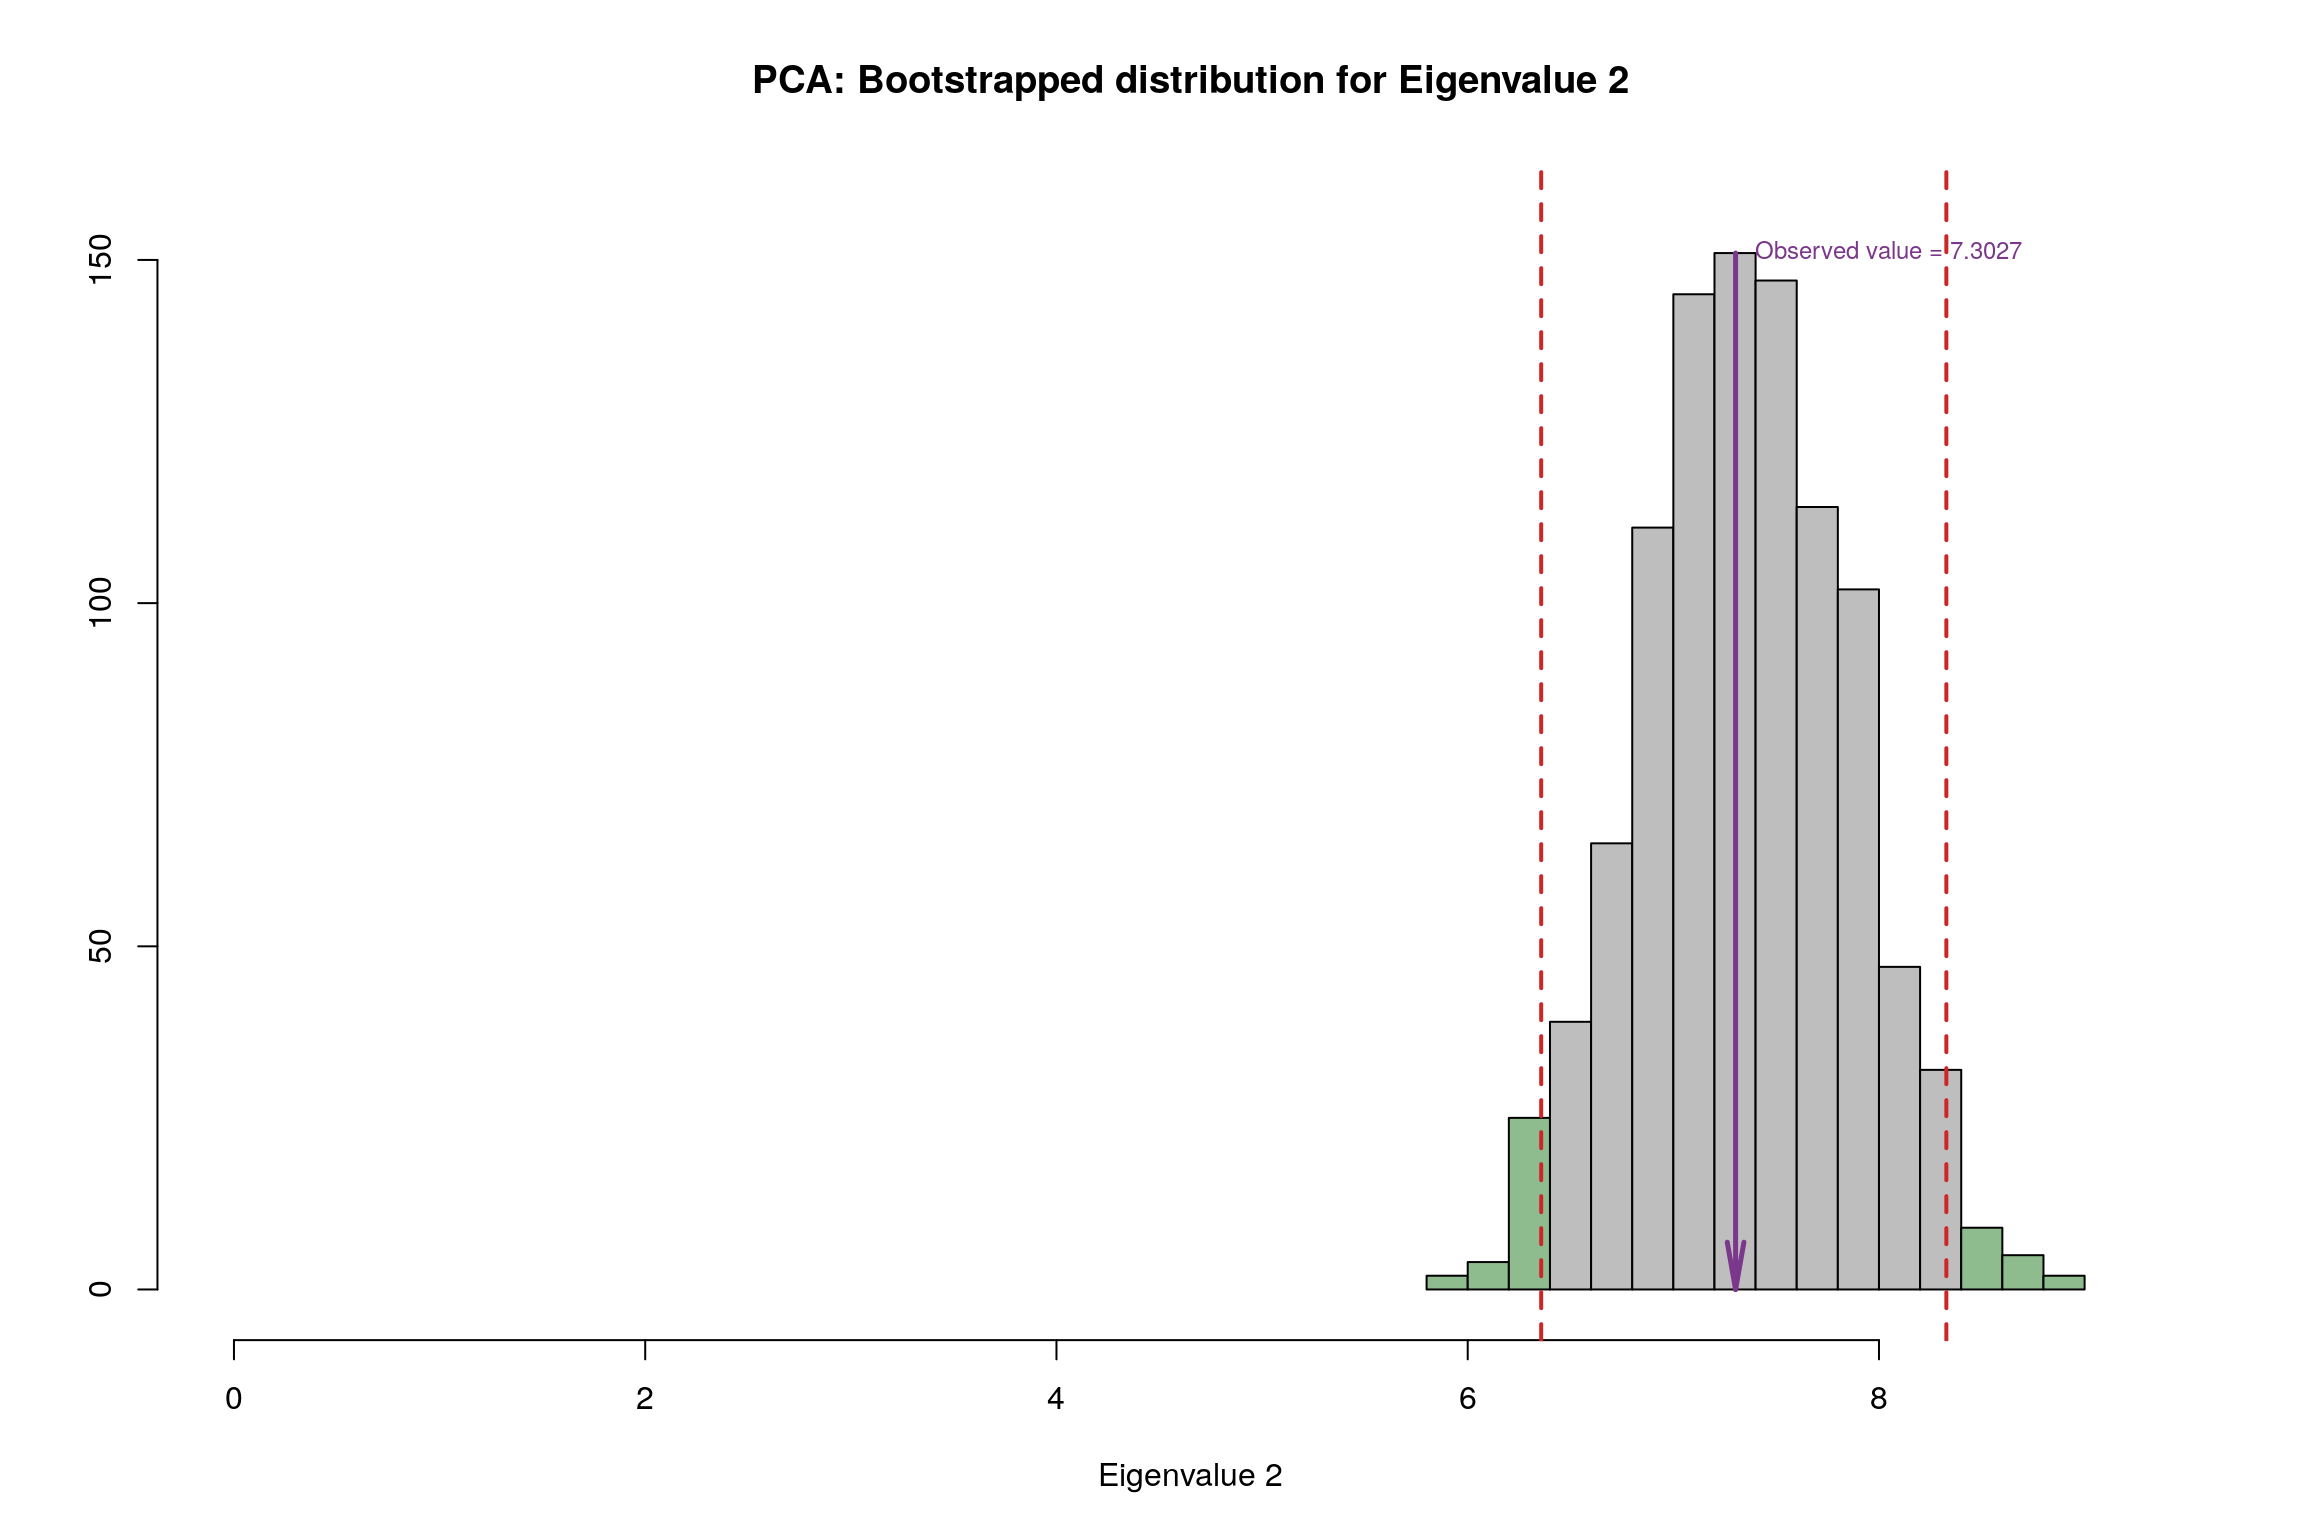
\includegraphics{Group1_Ritesh_Malaiya_PCA_Inference_World_env_vars_files/figure-latex/unnamed-chunk-18-2.pdf}


\end{document}
